
\chapter{Haptic Experience Design}
\label{ch:hapticianinterviews}

\inlineHeading{Preface} \osE{In }Chapters \ref{ch:hapticinstrument}-\ref{ch:applications} \osE{we} take a design perspective, investigating by doing.
The VT design tools each \osE{enabled} short in-lab sessions of design, which we could study directly; however, this approach lacks external validity.
Proxy design in \autoref{ch:hapturk} and the focused design projects in \autoref{ch:applications} offered ample opportunities to gain implicit knowledge about design; these results are ecologically valid but specific to only one group (our lab).
To triangulate both these approaches, we study the wider community: expert haptic designers in the wild.
Here, we report findings from six interviews with expert haptic experience designers, augmented by a workshop we coordinated at a major international haptics conference.
\osE{We found themes at three levels of scope: 1) the holistic nature of haptic experiences, 2) the collaborative ecosystem in which hapticians works, and 3) the broader cultural context of haptics.}
\autoref{ch:hapticianinterviews}\footnote{This work has been prepared as a manuscript and is presented as one.} both grounds our work and serves as a capstone: we define and characterize \haxd as it occurs in practice, codify challenges for \haxd, and develop recommendations to further develop the field that are grounded in this new understanding of designers.
We conclude with a vision for how \haxd might manifest in the upcoming years.

\section{Overview}
From simple vibrations to roles in complex multimodal systems, haptic technology is often a critical, expected component of user experience -- one face of the rapid progression towards blended physical-digital interfaces.
%% \kmC{??:especially as technology further blends the physical with the digital.}
Haptic experience design is thus now becoming part of many designers' jobs. We can expect it to present unique challenges, and yet we know almost nothing of what it looks like ``in the wild''
% However, the design process for haptics \kmC{awk: remains unstudied in the wild.}
%Between the rarity of professional haptic designers and the youth of the field, 
due to the field's youth and the difficulty of accessing practitioners %those practicing it
in professional and proprietary environments.
% the unique challenges of creative haptic design are not well characterized or understood.
%In this paper, we document and articulate the specific needs of haptic experience design differentiating it from sister fields of graphic, sound, and UX design.
In this paper, we analyze interviews with six professional haptic designers to document and articulate haptic experience design, observing designers' goals and processes and finding themes at three levels of scope: the holistic, multimodal nature of haptic experiences, a map of the collaborative ecosystem, and the cultural contexts of haptics.
% and suggest recommendations for supporting designers.
% Our findings are grounded in interviews with six professional haptic designers. 
% We supplement these interviews both with a survey and feedback from a workshop at a top haptics conference, and with reflections on our own experience designing both haptic experiences and haptic design tools.
%
Our findings are 
augmented by %further developed through % a survey and % redundant?
feedback obtained in a recent design workshop at an international haptics conference.
%, resulting in a description of haptic experiend design activities, a set of concrete challenges facing haptic experience designers and recommendations to help conquer them.
%Reflecting upon this data through the lens of our group's own experience of 20 years of designing both haptic experiences and haptic design tools, we have 
%encapsulated haptic experience design's process goals, collaborative ecosystem explicit recommendations for how tools can better support haptic and multimodal designer.
 % kmE
We find % show
that haptic designers follow a familiar design process, but face specific challenges when working with haptics. 
We capture and summarize these challenges, make concrete recommendations to conquer them, and present a vision for the future of haptic experience design.


\section{Introduction}
\noindent 
Haptic feedback provides value in several ways, especially accessibility~\citep{Bliss1970}, low-attention feedback~\citep{MacLean2009}, and motor skill training~\citep{Milot2010}.
Recently, high-fidelity haptic technology has expanded % emerging as a critical part of wearables, automobiles, and new media
user experience. %, especially with wearables, automobiles, and new media.
% Expressive actuators are increasingly deployed in consumer products like Apple's laptops (apple.com), wearable devices invite eyes- and hands-free interaction, and fabrication techniques further blur the distinction between digital and physical.
%where haptic experiences have shown promise in a diverse set of interactive application domains.
Emotional therapy~\citep{Yohanan2011affectdisplay,Vaucelle2009}, education~\citep{Sato2008}, and entertainment~\citep{SchneiderAsiaHaptics2014} are increasingly employing haptic feedback. % interactions [].
% Exciting new technologies, such as variable friction displays [] and ungrounded force illusions [] have the potential to produce compelling sensations in consumer products.
Technological advances enable more compelling haptic sensations in consumer products by making it possible to render variable friction on direct-touch surfaces~\citep{Levesque2011,Winfield2007}, and produce forces without needing to ground devices to a table or wall~\citep{Culbertson2016,Winfree2009}.
% Wearables especially have pursued this, with devices like the Apple Watch [] and Pebble (?) making haptic actuators a priority.
Even commodity vibrotactile displays are increasing in expressiveness, with high-quality actuation a priority in devices like the Apple Watch (\url{www.apple.com}) and the Pebble watch (\url{www.pebble.com}), although
often at the cost of painstaking and costly design effort.
Touch is now increasingly studied within market research because it improves the quality of product opinions and encourages consumer purchases~\citep{Jansson-Boyd2011}.
Part of the power of touch is its emotional, visceral~\citep{Norman2004} value with it has within a design, giving haptics a close relationship with user experience.




\begin{figure}[t]
    \centering
    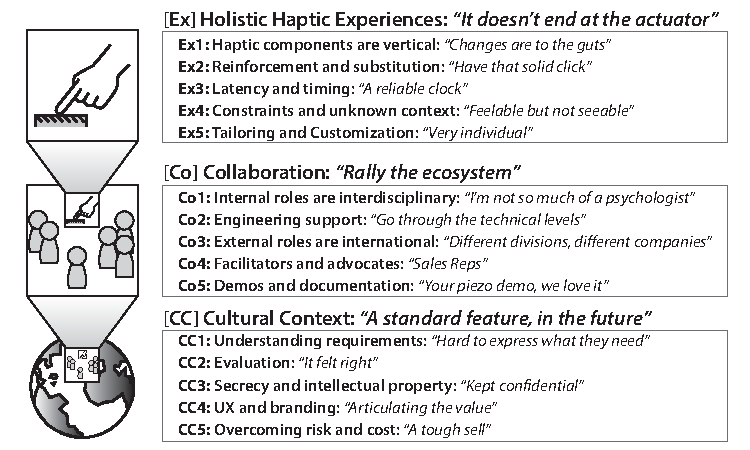
\includegraphics[width=1\textwidth]{Haptician-Grounding-IJCHS-2016-08-01-thesis}
    \caption{Our three themes, each exploring different levels of scope through 5 emergent sub-themes.}
    %\kmC{07.20: text is a little cramped, upsize and spread out slightly? And section numbers have changed.}
    \label{fig:themeoutline}
\end{figure}




\subsection{Haptic Experience Design (\haxd{})}
\noindent
We define \haxd\ as: % ``haptic experience design'' (\haxd) as:
\begin{quote}
\it The design (planning, development, and evaluation) of user experiences  deliberately connecting interactive technology to
% intentionally involving both interactive technology and
one or more perceived senses of touch, possibly as part of a multimodal or multisensory experience.
\end{quote}
Our focus is on gaining a better understanding of the workflow and processes currently used by \textit{hapticians}\revOne{. We define a haptician as:}

\begin{quote}
\revOne{\it One who is skilled at making haptic sensations, technology, or experiences.}
\end{quote}

\noindent
\revOne{We use the term ``haptician" to capture the diversity of people who currently make haptics, and the diversity of their goals.
Many people with a need to design haptics may not have formal design training, and may focus on subsets of the entire experience, \eg, technical demonstrations or creating stimuli for psychological tests.} %, the people who practice \haxd{} as part of their day-to-day work.
We describe \revOne{two studies examining} how contemporary hapticians design haptic experience\revOne{s} for use in real-world products. We begin by identifying current obstacles to good \haxd{} and the target audience for our work,  then provide a roadmap to the rest of the paper.

\subsection{Obstacles to Design} 
\noindent
The academic literature suggests many challenges to design for haptic experience.
%However, % despite the increasing presence of haptic technology, 
Haptic content remains scarce and design knowledge is limited.
% including 
Some issues are technological, arising in the hardware and software, such as highly variable hardware platforms and communications latency~\citep{Kaaresoja2014}. 
Other issues are human-centered, arising from individual user characteristics in perception and preferences:
% individual differences in 
low-level perceptual variation~\citep{Lo1984}, 
responses to programmed~\citep{Levesque2011} and natural~\citep{Hollins2000} textures, 
% the effect of aging 
sensory declines due to aging~\citep{Stevens1992,Stevens1996}, 
and  varied interpretation and appreciation of haptic effects and sensations~\citep{Seifi2013,Seifi2015} -- often because of personal experience~\citep{Schneider2014}.

These research findings are reinforced by many interactions the authors have had with practitioners in industry.
\revOne{We suspected} that there are many challenges related to haptics\revOne{,} % that face industrial designers,
but \revOne{had} little direct evidence to back this up and guide our research\revOne{.} %,
%still rely on indirect knowledge.
% Many haptic applications are built upon realistic physical models, but must still be fine-tuned. % and improved.
% \kmC{?? slc: Non-photorealistic } %% cross-modal analagy doesn't quite work as written. Abstract? Non-realistic? Techniques to create abstract signals (as opposed to high-fidelity recreations of a sensation found in the real world)
% techniques to create, \eg, vibrotactile feedback are even less understood.
% Though HCI researchers have long pursued haptic feedback and shown improved performance in various domains [], strict application of HCI design methods fail when applied naively to haptic-driven designs, and the specific challenges of designing haptic technology are many yet poorly documented.
% From an impoverished language [] to collaborative barriers []
\revOne{We} further suspect\revOne{ed} that it is somewhat rare for professionals to design haptic experiences explicitly rather than doing so in the course of larger design efforts\revOne{.}
We \revOne{thus conducted two studies} of the workflows used by designers when they are engaged in \haxd{} -- something that has been largely unexplored in the literature.

\textbf{In our \revOne{studies}, we take a first in-depth look at haptic designers' experiences to describe \haxd, identify  unique challenges, and connect \haxd to other fields of design}.
%\kbC{What are we correcting, especially if we have already confirmed? I would think formulate, confirm, and elaborate might be better.}
%\osC{We found ourselves in a chicken-and-egg situation, motivating this study by with expected obstacles and claiming found obstacles as the result. We had some ideas formulated going in from the literature and from practicing \haxd ourselves.}
%\kbC{I don't think this addresses my concern. Oliver's answer makes sense, but the text does not reflect this. The text only mentions ``correct'' without any indication whatsoever of what it is that is being corrected (and we do not say what he says in his comment, which is that we went into the study with a set of challenges in mind. In fact, the text suggests that we did not have a list in mind, but rather we set out discover what they might be.}
%\osC{Opening up chat for back-and-forth. Thoughts on the above?}
%\kbC{I have never used Chat in ShareLaTeX and cannot figure out how. I click on the Chat icon and things move around, but I see no chat area. Is there one?}
%\osC{Speech bubble in upper right is the chat button, the area is off to the right as another pane. Just sent email w/ screenshot if it helps.}
We focus specifically on \haxd instead of the more general notion of ``haptic design,'' 
%\osC{Might argue for moving this back to the definition. Makes sense here for setting scope, but I see it as also an important definitional distinction.}
which can also refer to design practices related to haptics not directly involving user experience, \eg, mechanical design of a new actuator or software design of a new control method.
Our definition encompasses pseudo-haptics~\citep{Pusch2011} and other illusions that trick a user into thinking haptic feedback is occurring without direct tactile or kinesthetic stimulation.
Much of what we discuss can also be gainfully applied to the design of tangibles, even with their lack of actuation, although we leave them out of our scope to focus on actuated interfaces\revOne{.}
%For brevity we sometimes use ``haptic designers'' to refer to haptic experience designers, while recognizing that beyond these pages this term may include other aspects of haptic design, including purely hardware and software components. We adopt the term ``haptician'' as shorthand for a practitioner of \haxd. % for both.% KM - for haptic experience design, not for the broader haptic designer. 
% \kmC{slc} % or, you could say ``HAX designers'' but perhaps a little too precious.


\subsection{Target Audience}
\noindent
We primarily target readers who are one step removed from \haxd, but who have other design, haptics, or business expertise relevant to haptics. %, such as non-haptic design experts, non-design haptic experts, and industry partners like entrepreneurs looking to work with haptics, or managers interacting with a haptic design group.

We expect that \textbf{\textit{haptic experience} design experts} (hapticians) will be unsurprised by the insights herein. % exposed here
% We hope that, % find our results familiar, % KM: don't feel like calling them 'results' in this context
% and hope 
Although they are not our primary audience, we hope that the articulated challenges and recommendations  will nevertheless still be useful for their practice because it consolidates their \textit{ad hoc} knowledge into a formal framework.


We expect that \textbf{non-haptic \textit{design} experts} will find our discussion of the specific challenges to \haxd informative because it reveals processes of design that are invisible or are taken for granted in other fields.
%their understanding of design broadened, especially with challenges that may not appear in more establish fields.
We also hope non-haptic designers might lend their expertise to accelerate
the generation of tools and techniques for creatively working with these complex interactive systems.

We expect that \textbf{non-design \textit{haptic} experts} will develop a further appreciation for how UX design is important for successful haptic technology, and will gain an understanding of how their devices or research findings are applied in practice.
The recommendations we provide may also motivate several avenues of either basic and applied haptic research that these experts could pursue.

We expect that
\textbf{industry practitioners} will gain insight into how the business case for haptic technology might be more quickly built.
This includes those already involved with haptics or similar technologies such as wearables, as well as those looking to become involved.
We believe our findings may help cultivate connections between the diverse stakeholders involved with % interacting with
\haxd, and that the challenges (and thus the opportunities) that we identify will inspire people to work more with this emerging modality.
%We think this will be valuable both for those involved with haptics or similar physical interactive technology like wearables, and for those looking to become involved.
%\kbC{The notion of industry partner is big with funding agencies (at least NSERC), but this isn't really a common term with the general international research community. I think ``industry practitioners'' or something equivalent might be better here. The second sentence in the paragraph suggests that these might not be current practitioners, but I think that it is OK to use the term because the qualification that follows makes it clear that we are talking about current or potential practitioners.}
% \osC{I support ``industry practicioner". Not sure about ``non-expert", I think there needs to be some qualifier for which industry practitioners, but they might be expert in things other than haptics/design.}
% \kbC{I was trying to continue the pattern of non-X, but since the first doesn't have this, the last doesn't need it either. I simplied to just ``industry practicioner."}

\subsection{Roadmap for the Reader}
\noindent
We describe \revOne{two studies} in which we sought to gain a solid understanding of % to shine a light into the dark land of
% shed light on 
\haxd as it is currently practiced ``in the wild'' by actual practitioners (hapticians) in their day-to-day work.
%: we document the challenges that are unique to or accentuated in haptic design, and apply  design thinking to those challenges.
%\kbC{I don't think the flashlight metaphor is a good one, especially the ``dark'' part!}
After a review of the existing literature in \textbf{Section~\ref{sec:lit-review}},
we report on the first \revOne{study} in \textbf{Section~\ref{sec:interviews}}: a grounded theory~\citep{Corbin2008} analysis of intensive interviews with six professional haptic designers.
% The grounded theory 
In our results, we describe observations about haptic designers' process 
% and has 
organized in three cross-cutting themes:
% \kbC{Are these actually levels, or are the ``aspects'' or ``components'' each of which is equally important? Are not these actually the ``themes'' we discovered? I used that term here.}
% \osC{Yes, let's make these themes (with sub-themes).}
% \kbC{Should ``goals'' have been ``tools'' in the previous?}
% \osC{No, although we have information on tools we could add to that theme. ``Adopted" might be wrong with ``goals" though...}
the complex, holistic nature of the experiences they design; 
the collaborative ecosystem in which haptic experience designers play multiple roles; 
and the influences of the cultural contexts in which haptic experiences are used and the value and risk this poses.
%
In \textbf{Section~\ref{sec:workshop}} we describe the \revOne{second study}, conducted in a workshop at a major international haptics conference (World Haptics 2015)\revOne{. The second study complements the first by collecting } quantitative and qualitative feedback from a broader sector of industry and academic designers regarding tool use, collaboration, evaluation methods, and challenges facing \revOne{hapticians}
%
% We supplement these interviews with a quantitative survey and qualitative suggestions from a workshop at a major haptics conference (WorldHaptics 2015), 
% % showing tools and groupwork more broadly in industry and academia. 
% following up on discovered themes on tools and collaboration with a broader sector of industry and academic designers.
In \textbf{Section~\ref{sec:discussion}}, we summarize and discuss our overall findings in three major areas:
%into a set of challenges and recommendations to improve the design process, and reflect upon how \haxd may evolve into its own discipline.
%\osC{slc}
%OS 2016.03.28 I do think we need to articulate that this is the *first look* at this field of design, and that it's *really hard* to find participants. Otherwise, it's going to look like a meager sample size.
\begin{enumerate}

    \item A description of current \haxd practice showing how it has already emerged as a distinct field of design.
    \item A list of challenges facing haptic experience designers, and some unique considerations \haxd requires compared to other more established fields of design.
    \item Recommendations for accelerating the development of \haxd as a full-fledged field of design.
\end{enumerate}

\noindent
We conclude with a few remarks imagining what a mature discipline of \haxd might look like in the near future.

% \begin{quote}
% Quotes can look like this!
% \end{quote}


%%%%%%%%%%%%%%%%%%%%%%%%%%%%%%%%%%%%%%
%
% Section: Related Work
%
%%%%%%%%%%%%%%%%%%%%%%%%%%%%%%%%%%%%%%
\section{Related Work}
\label{sec:lit-review}
\noindent
In this section, we discuss key elements of contemporary thinking about user experience design (UX design or XD) and a specific approach known as ``design thinking.'' We then broadly review haptic technology (hardware and software) and relevant aspects of human perception before providing a critical summary of previous efforts to understand and support \haxd. 
% \kmC{slc} 
%% KM 06.06.14 Start this section with some rationale for the two major subsections, and for ordering them this way (existing tools, and insights from other design fields). At first I was thinking it should be reversed, but could see either way.
%% Also you've begun with some definitions on what haptics are. Probably should give this a section heading, and think more carefully about how far you want to go with it and what is the point of having it there. One possible point, for example, is the high diversity of both the haptic sense (multihaptics) and the high diversity of devices targeting those different sensory receptors. this underlies one of the big challenges. 

%\kmE{16.07.14: This section needs considerable focusing. It lacks a purpose; I'm not convinced about why you've chosen to talk about these particular things, which seem almost picked at random, and discussed in ways that are not well related to paper objectives. Pause and rethink why you've chosen to include THESE topics: why are they the starting point, and why are the ones out of many aspects of user design that matter now? How do they set you up? What would be lost from your logical development and its foundations if you deleted them? What would reviewers object to if you started out cold with these terms?}

\subsection{Design Thinking as a Unifying Framework}
\noindent Design thinking is % has become 
an empowering way to approach technology and user experiences.
At the heart of this practice is the rapid generation, evaluation and iteration of \textit{multiple} ideas at once~\citep{Buxton2007}. % focused on rapidly generating, evaluating, and iterating on multiple ideas.
There are several general design activities that we observed in our participants that reflect design thinking, most notably, problem preparation, sketching-like iteration, and collaboration.

Many advocates of design thinking refer to an explicit problem preparation step preceding initial design~\citep{Schon1982,Warr2005,Shneiderman2000}, 
%Also known as the ``problem setting''~\citep{Schon1982}, ``analysis of problem''~\citep{Warr2005}, or ``collect''~\citep{Shneiderman2000} step, problem preparation
which involves ``getting a handle on the problem'' and drawing inspiration from previous work.
Designers find value in this stage because creative acts can be accurately seen as recombination of existing ideas, with a twist of novelty or spark of innovation by the individual creator~\citep{Warr2005}.
This stage draws from the designer's experience, including their understanding of the \emph{domain} (symbolic language of the field)~\citep{Csikszentmihalyi1996}, and the ability to \textit{frame} a design problem to match it to their repertoire, their their collected professional (and personal) experience~\citep{Schon1982}.
External examples are especially useful for inspiration and aiding initial design~\citep{Herring2009,Buxton2007}.
Early and repeated exposure can increase creativity, although late exposure carries a risk of conformity~\citep{Kulkarni2014}.

Later in this paper, we describe the evidence we found in our study that haptic designers' work naturally includes a dedicated problem preparation step, \eg, by employing collections of examples in a number of ways.


%\kmC{This section looks like an awkward cut-paste. In first para, you're describing parallelism, which is different than hands-on (and also seems to be an important tenent of design thinking; does it even belong here?). Then, you talk separately about sketching, with no clear bridge - which doesn't clearly connect either to hands-on-ness or to parallelism. I see sketching as epitomizing early-stage rapid exploration, as well as communication; but there is nothing specifically hands-on about this. Connect the dots better; at end, make sure to relate haptic technology to parallelism as well as to sketching. Make clear what you mean by 'hands on' - why is it a term you've brought up here in the background section?}

\textit{Sketching} is another critical design activity. It supports ideation, iteration, and evaluation. %, and multiple ideas.
Here, more generally than  pen and paper, we refer to general techniques to suggest, explore, propose, and question \citep{Buxton2007}, including physical ideation \citep{Moussette2010}.
%\kbC{ ADDRESSED -- I think we \emph{must} have a working definition of sketching, in part to ensure that readers do not take it to mean literally sketching a drawing with a pencil. The way we (and others) are using the term is to describe low-fidelity, incomplete descriptions of possible designs.}
Some researchers declare sketching to be the fundamental language of design, much like mathematics is considered the language of scientific thinking~\citep{Cross2006}.
Sketching is rapid and exploits ambiguity, allowing partial views of a proposed design or problem.
Detail can be subordinated, allowing a designer to zoom-in, solve a problem, and then
abstract it away when returning to a high-level view.
It can also support multiple, parallel designs, delaying commitment to a single design~\citep{Hartmann2008,Resnick2008}.
%, whilein groups, sharing multiple designs improves variety and quality~\citep{Dow2011}.
%\osC{cut this paragraph - should some of it be incorporated?}
The fluidity and \textit{ad hoc} nature of sketching extends to software tools: designers must be able to rapidly undo, copy and paste, and see a history of progress~\citep{Resnick2008}.

We discuss techniques for haptic sketching in prior work to support \haxd, and find major barriers to achieving fluidity that were identified by participants in our study.


\textit{Collaboration} improves design.
%Some argue that collaboration is inherently necessary: Csikszentmihalyi claims that creative acts must, by definition, be assessed for value~\citep{Csikszentmihalyi1996}.
Involving more people increases the potential for generating more varied ideas~\citep{Warr2005}, and is recognized as being important for creativity support tools~\citep{Resnick2008,Shneiderman2000}.
Although group dynamics can influence the design process negatively, proper group management and sharing of multiple ideas quite often results in more creativity and better designs~\citep{Herring2009}, and can even influence the work of crowds~\citep{Dow2012a}.
Collaboration can be categorized by intent, such as informal conversations with colleagues or widespread dissemination~\citep{Shneiderman2000}, or by physical and temporal context: collocated (collaborators in the same location) or distributed (in different locations), and synchronous (simultaneous) or asynchronous (at different times)~\citep{Ellis1991}.

We find these categorizations useful to identify where collaboration can break down for haptic design, especially remotely, asynchronously, and with limitations on informal or widespread sharing.
In Section~\ref{sec:interviews:collaboration} we present the first data-informed description of collaboration in \haxd. %the \haxd's collaborative ecosystem. 
%\kbC{Have we said what a collaborative ecosystem is? Are readers supposed to understand the term ``ecosystem'' as we are using it? I think it is a bit of jargon.}
%Many of these \kmC{which?} contexts require extra consideration \kmE{when being enaged in the pursuit of designing haptic applications.} % haptic technology.

%\kmC{Again, this reads like a cut-paste grab bag. Last 'relating' para is not convincingly connected or built upon the first parts. And once again, as a reader I'm not convinced about why we've bothered to address this topic. Why is it important? I think: Haptic design needs collaboration to thrive, like any other design discipline. But, there are some specific obstacles to it. We've exposed these obstacles, and the harm they do, in our [first known] analysis, which is na important first step towards addressing them.}


%OS 07.28 CUT
% In this work, we adopt an embodied perspective, \kmC{Clarify how this relates to Design Thinking.}
% viewing cognition, and thus design, as an activity that occurs both in physical and social worlds \kmE{[planes??]}~\citep{Dourish2004,Hutchins1995}.
% This perspective is particularly appropriate for \haxd: \kmE{it is both well aligned with} % as it matches 
% recent views of interaction design~\citep{Klemmer2006}, \kmE{and is also well suited to} % and suits
% the physical, embodied nature of haptic technology and \kmE{applications}.




\subsection{Haptic Perception and Technology} \noindent
Haptic technology is typically separated into two broad classes based on the complementary human sense modalities: \emph{tactile} sensations, perceived through the skin, and \emph{proprioception}, or the sense of body location and forces; the latter includes \emph{kinaesthetic} senses of force and motion. 
% \osC{Karon, I'm at a loss for a concise way to introduce and distinguish proprioception and kinaesthetic sensing. Any recommendations on phrases or places to look for definitions?} \kmC{08.01: this is good enough.}
On the human side these are further subdivided into different perceptual mechanisms, each targeted with different actuation techniques.
We  overview the complexity of the different senses that make up touch,
 then describe common actuation technologies for these senses, focusing on those mentioned by participants in our study.
%\kbC{ADDRESSED -- Here and earlier you are looking ahead to the study. In this case, I think it is a bit annoying because the reader has not yet heard enough about the study to know whether you are or are not focusing on the most relevant actuation technologies. Do you need to qualify this? Why not do that globaly, at the start of the section, and then not mention it again? My edit tries to deal with this.}
Finally, we review major application areas that use haptics for both utility and emotional value.




%Here, we focus on technologies most relevant to those discussed by our participants.
%
%\kmC{sounds here like you're not going to talk about perceptionn (but you do). Set up better, including a sentence indicating why you're including this material (in particular, this subset of material)}
%More detailed introductions can be found elsewhere, for example~\citep{Hayward2007,ChoiKuchenbecker2013}.
%My three in-depth case studies will focus on vibrotactile sensations for two reasons: 1) they represent a diverse class of soon-to-be consumer-facing devices, and 2) they can be passively experienced, simplifying the interaction model (we do not need to design for input).

%\kmC{high level for rest of this section: generally it's good material included, but same reaction as elsewhere: needs to be given a purpose and strategically connected to the rest of the document. For this section, I expect you'll be wanting to prepare the reader for the arguments of why and how haptic design needs to be different from, e.g., visual and auditory. If that's the case, it might be useful to draw comparisons and contrasts between the senses and then showing how (or at least, set up showing later) how this will impact tools. I DONT think you have space for a general tutorial on perception. This isn't a textbook. You need to be judicious, and let people know why you're telling them this stuff.}

Human perception of touch is synthesized from the tactile and proprioceptive senses, and is influenced by vision and hearing.
%\kbC{We seem to be switching between proprioception and kinaesthetic. Are these interchangeable? Why switch back and forth?}
%\osC{Tried to explain this above; might be easiest to ignore the distinction and just pick one of ``proprioceptive" or ``kinesthaetic", this audience is likely not picky.}
Tactile sensations rely on multiple sensory organs in the skin, each of which detect different properties, \eg, Merkel disks detect pressure or fine details, Meissner corpuscles detect fast, light sensations (flutter), Ruffini endings detect stretch, and Pacinian corpuscles detect vibration~\citep{ChoiKuchenbecker2013}.
Proprioception, the sense of force and position, is synthesized from multiple sensors as well: the muscle spindle (embedded in muscles), golgi-tendon organ (GTO) in tendons, and tactile and visual cues~\citep{Kandel2000}.
Humans use these senses together to learn about the world, \eg, stroking, bending, poking, and weighing objects in active exploration~\citep{Lederman1987}.
Haptic perception is also heavily influenced by other senses.
In the classic size-weight illusion~\citep{charpentier1891analyse}, when two weights have the same mass but different sizes, the smaller is perceived to be heavier, whether size is seen or felt~\citep{Hayward2016}; similarly, sound can affect how a texture feels~\citep{Hayward2016}.
Interactive systems can exploit cross-modal perception to reinforce or improve haptic sensations. To be effective, these effects need to be temporally synchronized, sometimes as closely as
20-100ms~\citep{Kaaresoja2014}.
% TODO include~\citep{levitin2000perception}.
%\kbC{ADDRESSED -- Nothing that precedes this suggests anything about timing. The size-weight illusion is not temporally based. So this is really a leap of faith on the part of the reader. This has switched from human perception in the real world to how human perception can be ``tricked'' into believing it is feeling something in the real world that is in fact artificial. I don't see how that fits into this section. In particular, what has the reader seen up to this point to provide any grounding for the 20-100ms requirement? Nothing!}
%\osC{Does this succeed?}
For more information about haptic perception, we direct the reader to~\citep{Lederman2009survey,Kandel2000,ChoiKuchenbecker2013}.



Haptic technology to produce stimuli for humans to feel is at least as diverse as the human senses that feel it.
%Several of our participants design 
Today, the most common approach is vibrotactile (VT) feedback, where vibrations stimulate Pacinian corpuscles in the skin, \eg, smartphone vibrations.
%\kbC{One again, we are jumping ahead to the study by talking about what participants do when we have not even introduced the study yet, much less the participants.}
VT actuators can take may forms.
Eccentric mass motors (sometimes ``rumble motors'') are found in many mobile devices and game controllers, and are affordable but inexpressive.
%An unbalanced mass is mounted on the motor, which provides dramatic shaking of the device.
More expressive mechanisms such as voice coils %  implemented in a variety of ways and 
offer independent control of two degrees of freedom, frequency and amplitude.
Piezo actuation is a very responsive technique that is typically more expensive than other vibrotactile technology.
% One of the more common and expressive is the C2 tactor, intended to directly stimulate the skin through contact or a thin membrane; the tactile animation project [] uses an array of C2 tactors.
%While tactors directly stimulate the skin,
Linear resonant actuators (LRAs) shake a mass back and forth to vibrate a handset in an expressive way; a common research example is the Haptuator~\citep{Yao2010}.
%Instead of directly stimulating the skin, this actuator typically shakes another device held by the user, such as a mobile device~\citep{Yoo2014} or pen~\citep{Culbertson2014}.
Currently, LRAs are increasingly deployed in mobile contexts (\eg, the Apple Watch Taptic engine).
Our participants also employ force-feedback, which engages proprioception.
Common force-feedback devices include Geomagic Touch (previously the Sensable PHANTOM) and Falcon devices, offering three degrees-of-freedom: force in three directions.
At other times, entire screens might push back on the user in a single degree-of-freedom.
These are only the most common feedback methods discussed by our participants.
Many other types of feedback can be used, \eg, temperature displays~\citep{Jones2002} or programmable friction display on touch screens~\citep{Levesque2011,Winfield2007}.

% \inlineHeading{Applications?}
% Simpler one degree-of-freedom devices are used in education, prototyping, and experimentation.
% Devices include the Twiddler (a haptic knob from UBC) and the HapKit (a low-cost paddle by the Stanford CHARM lab).
% %the latter is used in the CyberHap side project.


%\subsection{Applications}
%An early cinematic use of haptic feedback was in a multisensory experience called \emph{Percepto} used for the movie ``The Tingler'' in 1959~\citep{IJsselsteijn2003}. %
%%G. Riva, F. Davide, and W.A. IJsselsteijn, ÒPresence in the Past: What Can We Learn from Media History?,Ó Being There: Concept, Effects and Measurements of User Presence in Synthetic Environments, IOS Press, 2003, Amsterdam, The Netherlands, pp. 17-40.
%Theater seats were equipped with vibrating devices that buzzed the audience during events in the movie.
%Current 4D theaters, rides, shows, and gaming arcades are equipped with sophisticated motion platforms (e.g. D-Box, http://www.d-box.com) that supplement visual scenes with subtle and synchronized movements.
%Large tactile transducers (such as Buttkickers, www.thebuttkicker.com) are also common with gaming and music content that shake the entire seat using the sound stream, therefore allowing users to feel `bumps' during musical beats and gameplay. 
%Custom editors (such as D-Box Motion Code Editor) and software plugins are provided to media designers that overlaid the visual and audio content with haptics, and allow designers to generate, tune and save frame-by-frame haptic content in an allocated track for it to play simultaneously with the media content. 

%In contrast to displacing the entire user body, recent multichannel haptic devices create percepts of dynamic and localized haptic sensations directly on the user's skin~\citep{Israr2011} and in the mid-air~\citep{Wilson2014}.
%% Designers (and researchers) for these technologies must have 
%Use of these technologies requires
%extensive programming experience, knowledge of hardware and background in haptic sciences to generate expressive and meaningful haptic content. 
%% Due to the lack of
%Without guiding principles or haptic libraries, content generation schemes are complex, device-specific and time consuming. 
%Recently, Schneider and colleagues introduced the tool ``FeelCraft'' for end users to create expressive haptic content using a library of \emph{feel effects}~\citep{SchneiderAsiaHaptics2014}.
%By tuning parameters of these effects, users could personalize haptic content, embed it in games and share effects with other users.
%Similar devices and authoring schemes are also developed for on-line social interactions using custom multi-actuator haptic devices~\citep{Kim2009,Tsetserukou2009,Paneels2013}.%Tsetserukou, D. and Neviarouskaya, A. iFeel_IM!: augmenting emotions during on-line communication. Comp. Graphics & Applications 30 (2009), IEEE, 72-80.
%

\subsection{Efforts to Establish \haxd as a Distinct Field of Design}
\noindent
Researchers have developed several approaches to support \haxd.
Some have directly applied design metaphors from other fields to haptics.
Others have built collections of haptic sensations and toolkits that facilitate programming.
%\kbC{ADDRESSED -- We need to say something about what an ``editor'' is in the context of haptics.}
A number of haptic editors, analogous to graphical editors like Adobe Illustrator, have emerged to support specific haptic modalities through parameterized models or other abstractions.
These approaches have developed focused understandings of particular aspects of \haxd, but they do not adequately describe the process as it is actually practiced.

There are many examples of designers drawing from other fields to frame the practice of haptic design.
% ``DIY Haptics'' categorize feedback styles and design principles~\citep{Hayward2007,MacLean2008}.
% ``Ambience'' is proposed as one target for a haptic experience~\citep{MacLean2009}.
% Haptic illusions can serve as concise ways to explore the sense of touch, explain concepts to novices and inspire interfaces~\citep{Hayward2008}.
Haptic Cinematography~\citep{Danieau2014} uses a film-making metaphor, discussing physical effects using cinematographic concepts and establishing principles for editing based on cinematic editing~\citep{Guillotel2016}.
Similarly, 
Tactile Movies~\citep{Kim2009} and
Tactile Animation~\citep{Schneider2015}  
draw from other audio-visual experiences, and Cutaneous Grooves~\citep{Gunther2002} draws from music to explore ``haptic concerts'' and composition as metaphors.
Academic courses on haptics are taught with a variety of foci, including perception, control, and design that provide students with an initial repertoire of pre-existing skills drawn from other disciplines~\citep{Okamura2012,Jones2014}.
These and other ways of framing \haxd{} have been incorporated into rapid prototyping techniques that allow for faster, easier iteration of haptic designs.
Simple Haptics, epitomized by \emph{haptic sketching}, emphasizes rapid, hands-on exploration of a creative space~\citep{Moussette2010,Moussette2011}. % with a design perspective~\citep{Moussette2010,Moussette2011}.
Hardware platforms such as Arduino (arduino.cc) and Phidgets (phidgets.com)~\citep{Greenberg2001}, as well as the recent trend of DIY haptic devices~\citep{Martinez2016,Gallacher2016,Forsslund2015}, encourage hackers and makers to include haptics in their designs.

%\subsection{Language of Tactile Stimuli}
The language associated with tactile perception (terms related to haptic sensation and how they are used), especially affective (emotional) terms, is another way of framing haptic design.
%The language of tactile stimuli has a long history in psychological studies~\citep{Okamoto2013}.
Many psychophysical studies have been conducted to determine the main tactile dimensions with both synthetic haptics and real-world materials~\citep{Enriquez2003,Okamoto2013}.
Language is a promising way of capturing user experience~\citep{Obrist2013}, and can reveal useful parameters, \eg, how pressure influences affect~\citep{Zheng2012}.
Tools for customization by end-users, rather than by expert designers, are another place that efforts have been made to understand perceptual dimensions using a language-based approach~\citep{Seifi2014,Seifi2015}.
However, this work is far from complete; touch is difficult to describe, and some researchers even question the existence of a tactile language~\citep{Jansson-Boyd2011}.
%There is a clear need to empirically investigate the subjective experience of touch-based interfaces, for which phenomenology is ideal~\citep{Creswell2013, Moustakas1994}.
%Start with hapticons, tactons, vibrotactile icons, Earcons, Auditory icons...
%Participants described two different sensations, one oscillating at 16 Hz and the other at 250 Hz.




	% Guest, S., Dessirier, J., Mehrabyan, A., McGlone, F., Essick, G., Gescheider, G., Fontana, A., Xiong, R., Ackerley, R., and Blot, K., “The Development and Validation of Sensory and Emotional Scales of Touch Perception,” Attention, Perception, & Psychophysics, vol. 73:2, pp. 531-550, 2011.
%



Meanwhile, software developers who want to incorporate haptics into their systems are supported by large collections of haptic sensations and programming toolkits.
Sensation collections most commonly support VT stimuli. 
The UPenn Texture Toolkit contains 100 texture models created from recorded data, rendered through VT actuators and impedance-type force feedback devices~\citep{Culbertson2014}.
The Feel Effect library~\citep{Israr2014}, implemented in FeelCraft~\citep{SchneiderAsiaHaptics2014}, lets programmers control sensations using semantic parameters, \eg, ``heartbeat intensity.''
%and Feel Effects provide examples for vibrotactile actuators, like those found in game controllers and mobile devices.
Immersion's Haptic SDK (immersion.com) connects to mobile applications, augmenting Android's native vibration library with both a library of presets, and on some mobile devices, low-level drivers for effects like fade-ins.
%\kbC{ADDRESSED -- What does this mean? Does the SDK extend the native library by using the native library as the low-level driver for higher-level constructs dedined in the SDK? Give some specifics to clarify this.}
%FeelCraft's plugin architecture connects feel effects to various media types~\citep{SchneiderAsiaHaptics2014}.
VibViz~\citep{Seifi2015} is a free on-line tool with 120 vibrations organized around five different perceptual facets.
Force-feedback environments tend to be supported through programming toolkits.
CHAI3D (\url{chai3d.org}), H3D (\url{h3dapi.org}), and OpenHaptics (\url{geomagic.com}) are major efforts to simplify force-rendering.
Table-top haptic pucks can use the HapticTouch Toolkit \citep{Ledo2012}, which includes parametric adjustment (\eg, ``softness'') and programming support.
% Immersion's TouchSense Engage is a software solution for VT feedback programmingdevelopers. 

Finally, several software-based editing tools support haptic design for different devices.
These tend to focus on VT stimuli or simple 1-degree-of-freedom force feedback.
Many editors~\citep{Enriquez2003,Swindells2006,Ryu2008,Swindells2014,Meyer2016,Schneider2016macaron}
%The Hapticon editor~\citep{}, Haptic Icon Prototyper~\citep{}, posVibEditor~\citep{}, Vivitouch Studio~\citep{}, and Macaron~\citep{}
use graphical mathematical representations to edit either waveforms or profiles of dynamic parameters (torque, frequency, friction) over time.
Of these, Vivitouch Studio~\citep{Swindells2014} offers the most integration with other modalities in games, and Macaron~\citep{Schneider2016macaron} is the most available tool (online and web-based). % justifying the 'most'
% \kbE{on-line, web-based tool}.
%\kbC{ADDRESSED -- The previous sentence used to use ``accessiblity'' but that term is used here to mean something else.}
The Vibrotactile Score~\citep{Lee2009} uses a musical metaphor, shown to be preferable to a programming metaphor as long as the designer has musical experience~\citep{Lee2012}. 
Mobile ``sketching'' tools like the Demonstration-Based Editor~\citep{Hong2013} and
mHIVE, a Haptic Instrument~\citep{Schneider2014} are useful for exploration, but not refinement.
Since iOS 5 (2011), Apple has let end-users create on/off vibrations as custom vibration ringtones.
Immersion's Touch Effects Studio lets users enhance a video from a library of tactile icons supplied on a mobile platform.
Actuator sequencing~\citep{Paneels2013}, movie editing~\citep{Kim2009}, and animation~\citep{Schneider2015} metaphors enable multi-actuator, spatio-temporal VT editing.
%More recently, Vivitouch Studio~\citep{Swindells2014} allows for haptic prototyping of different effects alongside video (screen captures from video games) and audio, including features like A/B testing for simultaneous comparison of haptic content and exporting of a haptic video channel.

Some of these tools are founded in an understanding of haptic designers' needs \citep{Schneider2015,Swindells2014} and begin to capture a slice of the \haxd process~\citep{Schneider2016macaron}, but they do not fully capture the context and activities of contemporary haptic design.


% The control of multi-actuator outputs has been explored by TactiPEd~\citep{Paneels2013}, Cuartielles' proposed editor~\citep{Cuartielles2012}, and the tactile movie editor~\citep{Kim2009}; the latter combined spatial and temporal control using a tactile video metaphor for dense, regular arrays of tactile pixels (``taxels''), including a feature of sketching a path on video frames. 
% % However, these approaches embrace the separate control of different actuators, rather than a single perceived sensation produced by the multi-actuator device, which we address with tactile illusions in.

% %The hapticon editor~\citep{Enriquez2003}, haptic icon prototyper~\citep{Swindells2006}, posVibEditor~\citep{Ryu2008}, and Immersion's Haptic Studio (www.immersion.com) use a graphical representation to edit either waveforms or profiles of dynamic parameters (such as, torque) over time.

% %Both emphasize exploration and broad manipulation rather than finely controlled end results.


% Haptics has often made use of metaphors from other fields.
% Haptic icons~\citep{MacLean2003} and phonemes~\citep{Enriquez2006} are small, compositional, iconic representations of haptic ideas.
% Touch TV~\citep{Modhrain2001}, tactile movies~\citep{Kim2009}, haptic broadcasting~\citep{Cha2009}, and Feel Effects~\citep{Israr2014} attempt to add haptics to existing media types, especially video.
% Musical analogies have frequently been used to inspire haptic design tools, especially VT sensations. %unique.
% The Vibrotactile Score, a graphical editing tool representing vibration patterns as musical notes, is a major example~\citep{Lee2012, Lee2009}.
% %The vibrotactile score provides an abstraction beyond low-level parameters and can draw from a musician's familiarity with the notation.
% Other musical metaphors include the use of rhythm, often represented by musical notes and rests~\citep{Ternes2008,Brown2005,Chan2008, Brown2006a}.
% Earcons and tactons are represented with musical notes~\citep{Brewster1993,vanErp2003}, complete with
% tactile analogues of crescendos and sforzandos~\citep{Brown2006}.
% The concept of a VT concert found relevant tactile analogues to musical pitch, rhythm, and timbre for artistic purposes~\citep{Gunther2002}.
% Correspondingly, tactile dimensions have been also been used to describe musical ideas~\citep{Eitan2010}.



%%%%%%%%%%%%%%%%%%%%%%%%%%%%%%%%%%%%%%
%
% Section: Description
%
%%%%%%%%%%%%%%%%%%%%%%%%%%%%%%%%%%%%%%

% \kmC{High level - tons of great stuff in here, but structure is not coming through clearly enough yet. SLC}
%% KM 06.14: I'm struggling to visualize structure, partly because of the non-optimal heading styles, but partly because I don't think we're quite clear yet on what the structure is. I've tried to add some clarity, but it's only halfway there, and may seem even more messed up. Can you go through again and think about where *you* want the structure to be?
%% Also, there are places where the Background could do some work to ground. For exmaple, nature of haptic sense (multihapitcs), essentially multimodal, ... We have a choice, let these things come from the designers, or state them up front as context for hearing the designers. My sense is that the latter is better, otherwise we can't choose how much to elaborate and it comes off as digression.

% \section{Interview Analysis: Haptic Experience Designers in the Wild}
\section{Part I: Interviews with Hapticians about \haxd{} in the Wild}
\label{sec:interviews}
\noindent
In this section, we present findings from \revOne{our first study}, a qualitative analysis of interviews with six professional \revOne{hapticians}.
% \kmC{?? Should this be 'hapticions'?)}

%\kmC{slc} % I wish for a little more elaboration on how you found these four categories. Did absolutely everything fit into them? Was it like an annotation cloud? Don't assume your reader is so familiar with grounded theory and phenomenology to not need this. 
% E.g., To what extent was there a top-down factor in finding this structure? It would potentially add validity to have an "other" section, where you mention things that didn't fit, because I can't really believe that everything it into these.

%\kmC{OS 07.15: I separated description of your designers into its own section, because this is more Method than Result and this was confusing. Then, the design process analysis that was originally a subsubsection of that part is now 3.2.}

%\kbC{ADDRESSED -- Is the following itemized list just a note to ourselves, or is it intended to be part of the final manuscript? It seems out of place. Why not use a standard APA-like framework that starts with a Participant sibsection (where you can profile the participants) and then proceed from there with very brief subsections for the rest of the Method section and then move into Results?}
%\osC{It was supposed to be an outline of the different sections and their themes. Might not be applicable any more; I've commented it out.}

% \begin{itemize}
% % \item[\ref{sec:interviews:designers: a description of our designers and the types of projects they discussed;
% \item \textit{\ref{sec:interviews:process} \haxd process:} 
% %descriptive observations of 
% how our designers structured steps and stages in their typical work patterns. % a description of our designers and outline of their process.
% \item \textit{\ref{sec:interviews:experience} Structure and characteristics of haptic experiences:} nuances of designing in this modality, such as complexity, multimodality, %complexity, multimodal nature, 
% %vertical design modifications, 
% and designers' resulting challenges and strategies.
% \item \textit{\ref{sec:interviews:collaboration} Collaboration:} a casting of the different stakeholders and the roles they might take within the \haxd process. % roles of haptic experience design, and related themes.
% \item \textit{\ref{sec:interviews:culture} Cultural context:} widespread understanding of haptic experiences, including value, risk, and pragmatics of haptics as they impact % affecting 
% designers, users, and customers.
% \end{itemize}


\subsection{Method}
% and their Situation}
% \subsection{Haptic Experience Designers \kmE{and Designer's Culture Context}}% and Interview Process} % and their Process}
\label{sec:interviews:designers}
% \label{sec:interviews:designers}
\noindent
%\kmC{Should `meet the designers' or `The designers and our methods' should get its own subsection?}
%\kbC{The following paragraph might be better as the start of the Method section, because it provides context. On the other hand, it makes more sent to put it in the Discussion subsection because it reflects back on the generalizability of the Results, which as yet have not been reported (that's why it should go into Discussion).}
%\kmC{07.15: What situation? missing a sentence - you go right into what's changed as of 2016. Alternatively, could say: "we note that these observations are drawn from 2012. .... (2016) the situation is SIMILAR, with the following exceptions:''}
%\kmC{Here, is it worth noting the isolation, lack of specialized training, ... or should we just stick with what has changed, and indicate that everything else is about the same?}
One researcher (the 
% \kmC{?? should this be first author?} second co-author
first author) analyzed the interview transcripts through grounded theory~\citep{Corbin2008} influenced by %with influence from
 phenomenology~\citep{Moustakas1994} and thematic analysis \citep{Ryan2003}.
%
% We group our findings in four subsections, found by looking at different levels of context~\citep{Corbin2008} to cluster themes:
The analyzing author, who was trained in qualitative methods, first transcribed interviews and then examined every participant statement, tagging each with relevant and recurring concepts and keeping written notes for reflection and constant comparison.
Emergent sub-themes (sub-categories) \citep{Ryan2003} were discovered using qualitative techniques of memoing, iterative coding~\citep{Corbin2008}, clustering and affinity diagrams~\citep{Moustakas1994}.
Statements were later grouped according to tags, organized using affinity diagrams and clustering, and iteratively developed with further writing and reflection.
%\osC{MORE? slc} % Is the preceding clear enough? I could also mention I used qualitative data analysis software, or add a reference to a useful paper ``techniques to identify themes" which also has valuable points for thematic analysis.}
% \kmC{1-2 additional sentences with this info good, but also okay without it in pinch.}
% \osC{Should the preceding few sentences be moved to ``Procedure"?} \kmC{I think it is okay here.}
The 15 sub-themes clustered into three themes (categories)~\citep{Corbin2008,Ryan2003}.
We describe the themes in \autoref{sec:interviews:process} after an introduction to the designers themselves and the
procedure that was followed for the interviews.
We delay a detailed discussion of the results until \autoref{sec:discussion}
so we can 
include
%compare the findings from the first part of the study with
the findings of the second part of the study,
%which are
presented in \autoref{sec:workshop}.

\subsubsection{Participants}
\label{sec:interview:participants}

\noindent
Six participants were recruited, 5 male and 1 female. Initial contact was by email from a list of potential interviewees developed by the researchers. We describe each in terms of experience and training, area of focus within \haxd{}, types of projects, and constraints or other factors that might situate or provide insight into the interview.
Experience and position are reported as of the interview year (2012).

%\begin{table}[htbp]
%    % \scriptsize
%    \footnotesize
%    \centering
%    \begin{tabular}{p{\textwidth}}
        %  \toprule
        \textbf{P1} (M, over 15 years of human factors experience, PhD) held a design and human factors position at major healthcare company.
         He worked with auditory alarms, signals, and emotional experience.
         Despite a focus on audio, he frequently related his work to haptics and works with physical controls, designing characteristics like force profiles and detents, and
         described the haptic and audio processes as being the same. %\osC{08.01woah, this might actually be a big point right here, include in Discussion?}.
         Working in health care means there are tight regulations that need to be followed, and a noisy, diverse environment.
         P1 used a number of psychology and human factors techniques, such as semantic differential scales, factor analysis, and capturing meaning.
%         \kmC{Team / collaboration context?}
%          \\ \midrule
          
        \textbf{P2} (M, 5-6 years in haptics, PhD) described two projects: his experience adding mechanical feedback to touch screens at a major automotive company, and his PhD work on remote tactile feedback, where feedback was displayed on one hand while the other interacted with a touch screen. P2's main concern is ``rich feedback'', communicating information like affordances to the user. This is both pragmatic, such as ``consequences'' of the button, and affective, aiming to have sensations ``feel right.'' P2 focused on button presses on a touchscreen, rather than exploring ``roughness'' of a touchscreen or other surface. 
        % P2 accomplishes rich feedback by recreating physical buttons on a touchscreen; he eventually hopes to create virtual buttons that go beyond the physical world. P2 provided feedback in two ways – tactile feedback from screen displacement, and remote tactile feedback. Dwell times are used to mimic force sensing and feedback in the former, while timing is used for reinforcement to effect the latter. In both case, there is an indirectness to the sensation/input, and timing is used to circumvent this. Latency, and timing, are critical. 
%     \\ \midrule
        
        \textbf{P3} (M, 10 years leadership experience with actuation, sensing, and multimedia, M.Eng.) worked at a company that sells actuators used to add haptics to technology (like a tablet computer, game controller, or mobile phone).
        P3 had 20-30 projects going on at any time, each with their own level of size, goals, constraints, and other contexts. His main goal was to sell a developed actuator (with several variants).
        % Companies (customers) provide an existing device they wish to augment with haptics, prototypes, mockups, or CAD designs of new devices, or receive an evaluation kit and work with the P3's company to establish their hardware needs. The augmented prototype is shipped back to the customer, often in a different overseas country.
%         \\ \midrule
        
        \textbf{P4} (M, 11 years of design, development, and analysis/simulation experience, PhD) also puts actuators into new form factors (\eg, touch screens in cars). When he worked, he had limited time and resources, so there is not much time to change things. %Getting the outer dimensions for a visual impression is important.
%         \\ \midrule
        
        \textbf{P5} (M, 12 years of haptics UX experience, M.Sc.) held a user experience leadership position at major haptics company that sells haptic control technology and content; he described mostly software solutions.
        %P5's company is concerned with \qqquote{rallying the ecosystem} to make haptics more widespread.
        His company worked with different domains, but most examples are from mobile phones (handhelds), with a brief mention of automotive haptic feedback.
        They worked with extremely high-end piezo vibration actuators with high bandwidth (frequency and mechanical), and delivered software solutions for Android to their customers: OEMs (original equipment manufacturers).
        He described handheld feedback as two different classes: confirmation haptics, like a vibration to indicate a widget has been used, and animations/gestural feedback, which is more complicated.
        % There are two classes of feedback he discusses: confirmation haptics, and animations/gestural feedback.
        % Confirmation haptics are the primary product that P5 describes, adding haptics to the Android UI stack for major mobile phone manufacturers.
        % These effects are haptic confirmations of button presses extended to other UI widgets like drop-down menus and swipes to \qqquote{giving the user information that something is going on that they don't already know}.
        % Dynamics haptics, e.g., animations and gesture-based haptics, are a more challenging class of effects to design, integrate, and describe, and are left for future products.
%         \\ \midrule
        % CONFIRMATION HAPTICS: The primary project P5 described was adding haptics to the Android UI stack. In this case, the customers are major mobile phone manufacturers. The main goal was to take confirmation haptics present in buttons and extend them to other UI widgets (drop down menus, swipes, etc.). The value in this is in "giving the user information that something is going on that they don't already know". This is obvious with buttons, but less obvious in other widgets (e.g., date picker). However, the date picker gave interest, excitement, and a "mechanical intuition" or confidence in the UI (this contrasts with information they don't know, IMO).
        % ANIMATIONS AND GESTURES (DYNAMIC HAPTICS): P5 also distinguishes confirmation haptics with another class of interactions: animations and gesture-based haptics, described together as "dynamic haptics" (cf. "confirmation haptics"). Integrating haptics to animation is a challenging software engineering problem; P5 describes one point where animations were removed from the "confirmation haptics" package right before release, due to this challenge, and then added to a different product with dynamic haptics. Gesture-based haptics are much more complex to design and to explain (to the OEMs).
        
        \textbf{P6} (F, 5-6 years in haptics, PhD) worked at a major car manufactur\osE{or}. %ing company.
        She primarily designed ``feel'' properties such as friction, inertia, and detents of physical controls inside automobiles.
        P6 also works on active haptic controls.
        Design aspects include measuring force vs displacement profiles and maintenance of a large scale haptic design specification repository that spans user and technical requirements.
        This haptic specification repository is used by many engineering and business stakeholders across many sites in different countries.
        
%        %  \bottomrule
%      \end{tabular}
%    \caption{Our expert haptic designer participants and their projects. Experience and position are reported from interview year (2012).}
%    \label{tab:designers}
%    \end{table}

%\osC{OS HERE Monday 8:12pm PDT, will upload sundry documents while KM finishes pass. Up to here looks pretty good.}


\subsubsection{Procedure}
\noindent
\revOne{Another co-author, trained in interviewing techniques,}
%\kmC{Ambiguity - slc} % KM 12.29: there is now ambiguity here, becuase of the elaboration on training of one author, the first author, added earlier. Now, it's unclear what this co-author's training was, and if it is the same as the other (wording suggests multiple were "trained"). I know I suggested toning down detail earlier, but I think we need a little more.  Confusion is exacerbated by unclear distinctions of training in terms of data collection, and of analysis (because the present paragraph moves quickly from collection into analysis, so multiple co-authors are involved at different stages). % I see at least two possible solutions, and am leaning towards first.
% 1. Include a paragraph (probably early in Methods) where the roles and training of the active experimenter team (namely, you and Colin) are laid out. Could refer to them thereafter as e.g. "analysis co-author" and "interviewer co-author". More heavy handed that is normal to see, but perhaps after all it is needed.
% 2. Follow example above (re Anaylzing author) and specify what the training of this co-author was, right here. "A different co-author, trained in ...")
% KM (earlier): I don't think it's usual to specify who did what to this degree. Since co-author number is ambiguous (does it include first author?), just leave it this way.
interviewed the 6 participants in April-May 2012 using Skype.
Each interview lasted 30-60 minutes and consisted of initial ice-breaker and general open-ended questions. %, then increasingly detailed questions about participants' processes.
%Interviews followed a semi-formal, structured qualitative inquiry process that allowed for followup. % on interesting points.
%% KM 06.14: The timeframe might need explaining; relevance is that times have changed a bit in the intervening 4 years. e.g., see below
\revOne{To both cover our initial research questions and allow for emergent findings, interviews were semi-formal: a single set of prepared questions were asked from most general to most specific, but the interviewer flexibly and opportunistically followed up on interesting points.}

Interviews with P2-P5 were fully recorded and transcribed. Interviews with P1 and P6 were collected only as interviewer notes. In the presentation of % When presenting 
our findings, double quotation marks (\textit{``...''}) denote direct transcription quotes for P2-P5 while single quotation marks (\textit{`...'}) denote interviewer notes for P1 and P6. % reported with . % due to technical difficulties with recordings.
%As such, results from P2-5 are reported with full quotation marks \textit{``''}, and P1,6.
% Section~\ref{sec:interview:participants} describes our participants and their projects.
\revOne{We use qualitative writing techniques like rich or ``thick" description \citep{geertz1973interpretation}, \emph{in-vivo} codes (where participants' words are used to describe concepts) \citep{Corbin2008}, and quotations to provide the reader with a sense of verisimilitude and give our participants a more direct voice.
For example, we use the word ``guts", from P3, to refer to the tightly-coupled internal components of a system (\ref{sec:interviews:experience}/Ex1).}

% \subsection{The Haptic Experience Design Process}
% \label{sec:interviews:process}

\subsection{Results}
\label{sec:interviews:process}
% \inlineHeading{Design Process Overview}
% \label{sec:interviews:process} \noindent
% Here we describe the design process through different stages: the beginning, iteration, refinement, and evaluation.
%
\noindent
Most of the emergent themes  that we identified persist throughout the design process (\autoref{fig:themeoutline}). %applied to \kmC{?various? SLC} % KM 07.20: clarify, many different points or each theme a different specific point?
 %points throughout the design process.
We found participants generally followed a process typical of experience design (UX)~\citep{Buxton2007} % followed a familiar process 
in which they first tried to gain an understanding of the design problem, then iteratively developed ideas and evaluated them.
% \kbE{For completeness}
We first outline these confirmatory observations on process, then go on to  report on the themes, our main findings.
Throughout, we cross-reference themes by section number and theme label (\eg, \ref{sec:interviews:collaboration}/Co5).
% linking them to the cross-cutting themes


\subsubsection{Observations on Design Process}
\noindent
Participants described the initial stages of a project as a time to establish and understand requirements, gather initial design concepts, and define or negotiate project parameters.
Designers often collected examples of haptics, such as mechanical buttons and knobs, for inspiration (\ref{sec:interviews:collaboration}/Co5), 
and  they gathered requirements -- both direct requirements for haptic designs (\ref{sec:interviews:culture}/CC1), and project parameters around the value, cost, and risk of haptic technology (\ref{sec:interviews:culture}/CC4,CC5).

% \textit{Examples} take many forms, including a collected “button board” for inspiration (P2), a guidebook of physical button force profiles (P2), a mockup device sent from the client (P3), reference buttons (P4), or a large library of vibrotactile effects (P5).
% Engineering parameters are sometimes hard constraints (orientation of the actuator), or sometimes a ``best guess'' from the customer on what they want, which can then be iterated upon (P4).

% \textit{Project parameters} are non-design concerns negotiated with customers, especially early.
% This includes establishing value propositions, cost and cost structures, and initial pitches, demos, and networking. %Sales reps (P3, described below), \kmC{??: tech days} to interested parties, and timelines all facilitate this process.
% The entire team sometimes meets together early (P6) to make sure everyone is on the same page.
%\qquote{P3}{demo parts to them, present business cases to them, and show them what they can do in order to gain market share, or increase their retail price when they add our technology}.
% We discuss these contextual parameters more in Section~\ref{sec:interviews:culture}.




% \subsubsection{Iteratively developing concepts}
% \noindent
P2-P6 explicitly referred to an iterative process. They all found different ways to fit it into their collaborative ecosystem and constraints.
As we elaborate below, prototyping and assessment in the physical medium of haptics has many challenges that set it apart from graphical or auditory domains even as designers navigate very common-place objectives. For example,
initial requirements were often not actually what clients wanted, and our designers would have to iterate (\ref{sec:interviews:culture}/CC1).
% P4 describes a situation where the customer provided engineering requirements, but \kmC{?? 1st prototype?: it} didn't feel ``right''; P4 and the customer then iterated rapidly in-lab over a day to find what did feel right, changing several best-guess low-level requirements.
% \textit{??Conventional UCD:}
P5's teams explicitly follow a conventional user-centered design process, iterating simultaneously on prototypes and their understanding of customer needs.
% \textit{Iterate by subsystem:} 
P3 sometimes has to ship mockups and devices back and forth with their customers (\ref{sec:interviews:collaboration}/Co5).
Each design problem faced by our participants had to be treated as a unique problem, with designers fine-tuning their design to fit the problem (\ref{sec:interviews:experience}/Ex5).
%(Does P3 iterate? They seem to ship only once…but they follow up with support.)
% Modularity is pursued to facilitate both iteration and later fine-tuning, through swapping in and out themes (P5), %[insert other example?] 
% %“and, uh, when, if we had known directly from the beginning where we would have ended, we would have ended with a smaller actuator module for uh, the demonstrator unit
% and different theoretical parameters are persued during iteration:
% \qquote{P4}{For the full application, we would have had to run through a few demonstrator units beforehand anyway, so it would not have made any difference [if we knew where we would end up]}.
%
% % \subsubsection{Refinement and fine-tuning}
% \textit{\kmE{Bespoke experiences:}}
% As we will elaborate in Section \ref{sec:tailoringandcustomization},
% our participants commonly tailored and customized their designs depending on the application.
% % All (?) participants indicated some kind of tailored product.
% \osC{slc -KM}
% % OS 2016.03.29 I wonder if there's some sort of analogy to clothing tailoring, e.g., "bespoke haptics", "tailored" haptics, "off-the-rack" haptics
% % The term 'bespoke haptics' has been used. I've seen it a couple of times, and like it... google gives this
% % https://www.deakin.edu.au/research/iisri/our-research/haptics-research
% % 2007: http://www.sciencebusiness.net/news/72255/Edinburgh-spins-out-joint-science-art-haptic-technology-company 
% % I think okay to give it without reference, but don't make a big deal of it. 
% \kmE{Application- and client-driven (?)} refinement and fine-tuning was baked directly into some participants' business models.
% P3's company sells a single actuator, with several variants, which are used based on the project needs;
% similarly, P4's actuators are customized depending on the context. P5's design team chooses a small set of effects from their libraries that represent the unique branding of an application.
% \kmC{[ground better:] Having haptic effects being effective} depends on the specific context of a project (both physical layout and social/use context).
%\textit{Evaluation:} our designers also 
Our designers used a variety of evaluation techniques to choose their final designs (\ref{sec:interviews:culture}/CC2).

We now proceed with our  cross-cutting themes, organized by scope (Figure~\ref{fig:themeoutline}): the haptic experience and its implementation (Section~\ref{sec:interviews:experience}), the designers' collaborative ecosystem (Section~\ref{sec:interviews:collaboration}), and implications from the wider cultural context of haptic technology and business requirements (Section~\ref{sec:interviews:culture}).



%%%%%%%%%%%%%%%%%%%%%
% Subsection: Systems solution challenges
%%%%%%%%%%%%%%%%%%%%%
\subsubsection{\textbf{[Theme Ex]} Holistic Haptic Experiences: ``It doesn't end at the actuator''}
\label{sec:interviews:experience}
% \begin{quote}
%  \end{quote
%\qqquote{It doesn't end at the actuator} %}
%
\noindent 
Context is crucial to experience at multiple levels, but is difficult for a designer to foresee or control. 
Aspects of context range from immediate, very local electromechanical environment (material properties, casing resonance, computational latencies), through the user's manner of touching the haptic element (grip, forces, longevity of contact), to the user's momentary environment, attention, and goals.
%and the endeavour they are engaged in around the time of the haptic interaction.}

%\kmC{07.20: first quote skews sense of this section. SLC.} % my problem with this first quote, nice as it is, is that it skews the reader towards expecting JUST local context. But you come back to larger context with Ex4. Can you adjust? Not sure of your intentions}
%OS 07.26 I'm not seeing it as skewed. Yes, it uses the word "actuator" which anchors the reader to local electro-mechanical context, but I think it applies more generally to other levels of context. Now, we do have an option for "systems solution challenges" but I still like "It doesn't end at the actuator".
%OS:0.7.28 I'm not convinced this quote skews the reader too much.

At the local end, the complexity of the haptic sense itself is a major factor in expanding the haptic experience design space substantially beyond what are usually its initial requirements -- for example, for the changing feel of a modal physical control in an automobile cockpit.
%
As we've discussed, 
the haptic sense is really a collection of subsenses~\citep{Kandel2000,ChoiKuchenbecker2013}, working together to construct an overall percept, \eg, material properties deduced from stroking, tapping, or flexing a surface or object~\citep{Lederman1987}.
% \kmE{This factor expands the haptic experience design space substantially beyond what are usually its initial requirements -- for example, for the changing feel of a modal physical control in an automobile cockpit. }
Grip, materials, dynamics as well as visual and audio aspects all play a part in the result.
%
\begin{quote}
\qquote{P5}{The problem is it doesn't end at the actuator, there's a lot to do with the case of the device, the mass of the device, the mechanical coupling between the device and the hand...this all comes into play because it's %, %you know it's 
a tangible experience, and so if there's mechanical resonances that get stimulated by the actuator that make it sound noisy, then it becomes a cheap experience, even if it has a piezo actuator.}
%and so this is all very important design consideration}.
\end{quote}

\noindent 
% This holistic, %, context-sensitive 
% \kmE{multisensory} nature of haptic experiences has implications for \haxd. 
Thus, designers both face multifaceted % multimodal 
constraints and have opportunities to circumvent those constraints. %, this is a double-edged sword. 
%Here, we discuss the nature of haptic experiences as vertical, multimodal systems.
We begin by discussing implications for implementation, wherein haptic components are directly related to the internal mechanics -- the ``guts'' -- of the system (Sub-theme Ex1).
% When designers can control these additional materials, they can enhance the experience.
% At other times, contextual factors offer constraints, or worse, are completely unknown.
% This also
Then, we move on to opportunities for improving design: strategies like reinforcement and substitution are powerful tools for haptic designers (Ex2). 
Timing is critical, enabling abovementioned opportunities while imposing constraints: designers must introduce no new delays and carefully synchronize feedback (Ex3).
However, the full extent of a sensory context is % multimodal contexts are
 sometimes uncontrollable or unknown, and at such times prevent designers from using their tricks (Ex4).
We finish this section by discussing how haptic experiences are often bespoke, 
tailored to constraints of known contexts, or customizable to unknown contexts (Ex5).
%This ``systems'' formation also slows iteration and makes latency and timing a major concern.
% Other parts of the system add complexity, might be out of the designers' direct control (e.g., the visual interface might be handled by another company), or might be completely unknowable (the grip of a phone or the surface it is on).
%Ultimately, the multimodal nature of haptics adds complexity and uncertainty.

% \kmC{07.22: on reflection, I'm tempted to drop the quotes from the EX headings. SLC} % the problem is they over specialize - the theme is more general than the quote, and it's confusing. They don't adequately capture it. This is true for most of them.


\begin{table}[htbp]
    % \scriptsize
    \footnotesize
    \centering
    \caption{Sub-theme summaries for the Holistic Haptic Experiences (Ex1) theme.}
    \label{tab:experience:holistic:overview}
    \fcolorbox{black}{lightgray}{
    % \begin{tabular}{p{0.03\textwidth} p{0.33\textwidth}p{0.55\textwidth}}
    \begin{tabular}{p{0.05\textwidth}p{0.37\textwidth}p{0.45\textwidth}}
        %   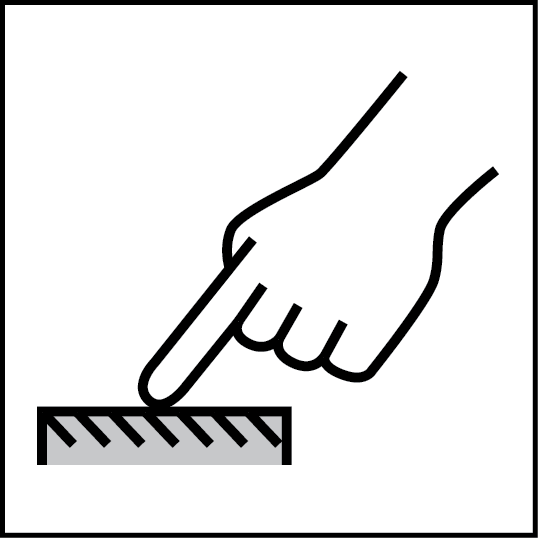
\includegraphics[height=0.3in]{figures/HapticExperienceLogo}
        %   & \textbf{Haptic Experiences}
        %   & \\
          \textbf{Code} & \textbf{Sub-theme descriptor} & \textbf{Explanation} \\
          \midrule
          \textbf{Ex1}
            & %\textit{``Changes are to the guts''}
            Haptic components are vertical
            & Changing a haptic component may influence the larger hardware/software system, and vice-versa. \\ \midrule
            
            \textbf{Ex2}
            &% \textit{``Have that solid click''}
            Tricks to create great feels
            & Haptic designers can improve designs and work around constraints through multimodal tricks. \\ \midrule
            
            \textbf{Ex3}
            & %\textit{``A reliable clock''}
            Latency and Timing
            & Without fast feedback and synchronized timing, haptic experiences fall apart. \\ \midrule
            
            \textbf{Ex4}
            & %\textit{``Feelable but not seeable''}
            Constraints and unknown context
            & Other modalities may impose constraints; constraints may not always be knowable. \\ \midrule
            
            \textbf{Ex5}
            & %\textit{``Very individual''}
            Tailoring and customization
            & Designers tailor their solutions to each application; end-users benefit from customization. \\
        
          %\bottomrule
      \end{tabular}}
    \end{table}



\themeHeading{Ex1}{``Changes are to the guts''}{Haptic components are vertical}
%\inlineHeading{``Changes are to the guts'' -- haptic components are vertical}
Haptic experiences are % created the actuating component interacting 
created when the actuating component physically interacts with other system components.
Changing a haptic component can thus affect the entire system's design, unlike 
%Changing a haptic component is thus a change to the \qquote{P3}{guts}, where the design of the entire system is affected.
%P3 contrasts this with 
many other upgrades, like improving memory in a mobile phone: \qquote{P3}{you get the impression every other month they have a new phone...but the guts of it do not change much}.
New phones often just have a faster CPU or more memory swapped into an essentially unchanged % the same 
system; but
 % upgrades can be as simple as adding a new memory chip.
%Unlike other components, like mobile phones, improving memory is quantifiable and fits into a dedi\textbf{}cated, comparable category; haptics requires a .
when adding or modifying haptic components, designers must consider the entire system including the physical casing, and possibly modify it as well:

\begin{quote}
\qquote{P4}{First we had to get the outer dimensions [of the prototype's case] roughly about right, to get the visual impression close to what it resembles later in the application}.
\end{quote}

\noindent This effect is bidirectional. 
% Both physical and non-physical elements influence each other.
Changing the size or material of the casing can have a profound effect on the sensation; correspondingly, any changes to the haptics will have an effect on the entire structure of the device.
% This is built into our designers' process:
Changes to software are also cross-cutting:
\qquote{P5}{we're digging into the source code of Android...we need to make sure that we have the right hooks in the right locations...that's a software architecture issue, right?}.


%, and changes in other components will affect the haptics, as described above.

% As we'll see, this has implications for both the iteration cycle (which is slower and more painful), risk for adding or changing haptics, and latency. \osC{TODO: discuss some quotations about changing software by P5, and some others for P2-4}


%SOFTWARE
%P5: P5: um, well it’s a little, I’m sure it’s different than usual switch design, because, or control design, because, we’re digging into the source code of Android, and trying to figure out what, how we could associate input events with feedback
% and so it’s, I guess it’s similar to mechanical control design, except that it’s all virtual, right, so now we have this event loop and we need to make sure that we have the right hooks in the right locations, and the right um, the right way to override existing behaviours, which Android already has some of, and the right way to enable this such that it’s easy to swap in and out effects in a theme context
% so to basically re-format the whole experience in one fell swoop, you know that’s a software architecture issue, right?
%P5: um, there was a few, um particularly around um, let’s see, around animated widgets, so I don’t know how familiar you are with Android but there’s some widgets that have animation controllers associated with them, and um
%  and that’s fine and that works great if you’re using a finger to interact with these things, but there are some controls which also can receive events from other parts of the system, notifications, or from other widgets, and if those are animated then you get into this kind of feedback loop, which makes the device kinda go crazy
%  and so we, we had to, you know, engineer our way around that but, it’s not a super hard, um, just, you know, engineering work





%
% Subsubsection: Advantages, multimodal tricks
%
% \themeHeading{Ex2}{``Have that solid click''}{Reinforcement and substitution}
\themeHeading{Ex2}{``Have that solid click''}{Tricks to create great feels}
% \kmC{07.21: alt name: ``Have that solid click'' -- Exploitation of mechanics and illusions} 

% \kmC{07.21: need to CLARIFY and GENERALIZE this theme. SLC} 
% (1) As noted when this theme was introduced: need to clarify if reinforcement, substitution are just examples of opportunities to use multimodal situation to improve design, or they are intended to be the full pallette of tools here. Need another sentence here setting this up.
% (2) 'have that solid click' signals a theme that focuses in on the effort of creating great feels. It doesn't convey any exclusive signal about multimodal tricks. imo, the illusions are just one way to get there. Others include high quality, responsive components; many illusions, both multisensory and the way the haptic element alone is programmed and engineered. I think this theme would be more transparent and interesting if you broadened, but make this scope more clear. 

% \kmC{07.21: The point about high bandwidth actuators and their contribution to feel, currently in Ex3, belongs better here. SLC} % as I note below under Ex3, the issues with simultaneity are only negligibly impacted by actuator responsiveness, and it confuses that point badly. Also see comment just above.

% \kmC{07.20: another aspect of context is manner of touching, but this hasn't been introduced adequately. 07.21: partially fixed; SLC} 
% [07.21: the rest of this comment is from an earlier pass... I've tried to bring manner-of-touching in better, not sure if it flows adequately yet.] Comes up in substitution below a little, and 'grip' above, but not prepared enough. Make sure the manner of the user's approaching, dwelling, impacting, stroking vs tapping vs gripping etc, are mentioned as part of the situation of the device. I'd use the example in play - car dashboard - to explain what is meant here.

\noindent
Haptic designers have an array of techniques to create great experiences, working around constraints and uncertainty.
The first step is to have a fast, responsive actuator when possible. % Haptic actuators themselves have become very fast and responsive.
Previously, creating good actuators was a goal for our participants:
\qquote{P5}{[what we] strived in the past significantly to do was to push the market towards high mechanical bandwidth actuators, so actuators that can respond in 15 milliseconds or less}.
Now, high-quality actuators are a main competitive advantage:
\begin{quote}
\qquote{P3}{High-definition feels over a very broad frequency range, with enough strength and small enough, and especially very fast response time, that's our business}.
\end{quote}
% \qquote{P4}{you get almost perfect perpendicular motion of the surface directed to the touch screen}.

As discussed in Ex1, the actuator does not determine the experience alone, but interacts with physical materials and non-haptic senses.
% \inlineHeading{``Have that solid click'' -- Reinforcement and Substitution}
When a haptic device's ultimate situation is known at design time -- like a car dashboard -- 
designers can modify 
properties of the larger physical system to improve the overall haptic experience:
%With complete control over the end product, materials and housing can be changed: 
\qterm{P6}{metal makes unwanted sound, so change it with a plastic}.
% Knowing the \kmE{where the device will ultimately be situated allows} % context, like a car dashboard, lets
The designer can also make a sensation more convincing with multimodal reinforcement, \eg, adding visual or audio feedback:

\begin{quote}
%Sometimes this is as simple as adding a audio click:
\qquote{P5}{%adding in some level of audio too, that also makes a huge difference...
%, especially in the automotive space...
%I work with some automotive people and they just, they
Need to have that
%, you know a,
solid [haptic] click at 150 [Hz] plus some audio at 300 or 400 Hz, which is going to give you that sense of quality, and, consistency across the whole dashboard}.
\end{quote}

When a known physical context has constraints, designers also use substitution to  enable or improve the haptic interaction.
P2 describes two such occasions, one for sensing input and one for displaying output.
%, both in an automotive application.
%One major limitations of haptic displays is that they don't always directly match the desired sensation context.
%In these situations,
%substitution is a critical tool for designers.
%In one case, %substitution makes up for sensor modality:
Because P2 could not sense input pressure, he instead used %Instead of sensing input pressure, temporal features like vibrations and
how long the user was pressing the screen (``dwell time''): % are used in place of spatial sensing like pressure and force feedback:
\qquote{P2}{we were substituting the forces that are needed on the actual buttons with dynamic dwell times}.
This was only possible because P2 had knowledge of \emph{how} the user would be touching the control, and thus could deduce that dwell time was a reasonable proxy for pressure.
%Alternatively, multimodal synthesis can make up for weaknesses in the display.
In another case, P2 could not actuate a touch screen, so he used tactile feedback on the other hand -- again, requiring knowledge of and considerable design access to the device's and user's larger situation; here, the steering wheel.


% \subsubsection{``A reliable clock'': Latency and Timing}
\themeHeading{Ex3}{``A reliable clock''}{Latency and Timing}

\noindent
One underlying requirement for great haptic experiences is responsive timing.
Feedback must be fast; modalities must be synchronized.
%\kmC{07.21: This whole thread strikes me as missing the heart of it - need to re-slice. SLC.} % There are two things here. 
% (1) actuator itself - responsiveness leads to expressiveness and being able to address a large, distinctive range of sensations, but it's a negligible part of simultaneity, i.e. timing issues / overall command-to-result pipeline. I THINK THIS POINT / QUOTES BELONG ELSEWHERE - probably in Ex2.
% (2) system computational latency. I think this is what this theme really should be about. It's huge, and gets worse when you are mixing systems. Timing is about the whole computational architecture of the integrated system, which inevitably includes disparate processing units, and very rarely will any other elements have msec level timing requirements - they will not be designed with haptic realtime requirements in mind. Chained together, they're very unpredictable. The fact that designers often can't know what the whole computational chain will be obviously makes things worse. 
% As written, this section comes off as naive understatement and misattribution of the actual problem. Even with the quotes you have, you can hit a lot harder by saying some of the above.
% \inlineHeading{Very fast feedback and a reliable clock -- Latency and Timing}
Effective reinforcement requires simultaneity and hence tight (millisecond) control over timing.
% To effectively use reinforcement, and to have effective haptic feedback, timing must be tightly controlled.
%Timing is critical to enable multimodal reinforcement and maintain the magic of haptics.
This is well established in the literature~\citep{levitin2000perception,Kaaresoja2014} and known to our designers:
\qquote{P2}{I think, audio feedback and tactile feedback and visual feedback has to happen at a certain time to have a real effect}.
%Because haptics are part of
%One stand-out result of systems modifications is that they are complex and have an major effect on component communication, latency, and timing.

Latency accumulates throughout the computational pipeline, with actuator responsiveness the very last stage and rarely the most impactful.
Designers must minimize computational delays wherever possible.
% now focus on introducing no new delays to the stack. % KM 07.21: note, this has ALWAYS been true - it's not some recent thing.
%when connecting with vertical components.
P2 describes unintentionally adding latency to one project: \qqquote{we had this Python program and Arduino and all this communication going on} and how he
\qqquote{threw out some of the serial communication which [had] made the whole thing a little slow}, and thus, the \qqquote{latency again felt right}.
Timing problems between components can happen at any time:
\qquote{P5}{we've gotten in situations before where we've been very near to completion in design projects, and for whatever reason we can't get a reliable clock, from the CPU, then the whole thing falls apart}.
%{P5}{um, cuz nothing is consistent, you have hiccups in the effects and, there's just no easy way psychophysically to bridge, a variable timer sensation}
% \osC{Need to add in quote or mention of fast actuators - components aren't the problem}

% \textbf{Hardware is not the problem, complexity is.}
% Latency is critical, and while good, fast actuators exist, designers can't add new bottlenecks. 
% Although responsive hardware used to be a problem (\qquote{P5}{[we] strived in the past significantly to do was to push the market towards high mechanical bandwidth actuators, so actuators that can respond in 15 milliseconds or less}), this is no longer the case:
% Haptic companies have become very good at creating good hardware:
% \qquote{P3}{high-definition feels over a very broad frequency range, with enough strength and small enough, and especially very fast response time, that's our business}\

% \osC{todo: fit this quote in}
% \qquote{P2}{on touchscreens you always want to be really fast if you input text or something, and on push buttons, normally you think of a large thing and you have to press it down and it take you several seconds to activate}


% \kmC{This last one (following) is about simultaneity and timing. Belongs in Ex3, but must connect it to the non-collation example started in Ex2. SLC} % This one is about SYSTEM latency, which you're coveringin Ex3. I'd swap it with the example now in Ex3 that does belong here - high quality actuators, really very little to do with latency but all about expressiveness and crispness.}
%
% With careful timing, %Because human brains
% the user perceives a single sensation, letting P2 actuate another location, \eg, the steering wheel:
When adequate simultaneity constraints are met, the user perceptually \emph{fuses} these non-collated events (activating a graphical element on a screen, and feeling a tick on the steering wheel) into a single percept:
\qquote{P2}{somehow you connect these two things, the action with the dominant hand and the reaction that is happening somewhere else}.
Haptic designers thus need access to the computational pipeline to circumvent physical constraints with multimodal tricks.

\themeHeading{Ex4}{``Feelable but not seeable''}{Unknown user constraints and context}
% \inlineHeading{``Feelable but not seeable'' -- Constraints and Unknown Context} % Lack of Knowledge}
\label{sec:interviews:constraints}
Haptic designers sometimes contend with unavoidable constraints emerging from physical context or application space.
Some constraints not only limit multimodal synergies, but go on to %tricks, but 
actively limit haptic display.
%The \kmE{larger context of a user's situation imposes constraints that the designer may not be able to control or leverage.} % may be unknown or uncontrollable haptic experience can limit the designer.
%Multimodal feedback is not always controllable, and sometimes actively constrains the designer.
%However, sometimes constraints remove the ability to use other modalities.
%
For example, eyes-free interaction in cars means that visual reinforcement is unavailable; indeed, visual movement may have to be avoided altogether for safety reasons.
P4 %uses audio reinforcement, but 
is tasked with creating a \qqquote{feelable but not seeable} sensation to \qqquote{avoid having to use visual feedback}, as \qquote{P4}{driver distraction is always a big topic}. 
% P4 had to actively avoid using visual feedback and rely solely on the tactile feedback of a moving touch screen, and actually make the motion unnoticeable visually.
This means P4 has limited control over his designed haptic sensation, as it cannot visibly move, but P4 can use audio reinforcement or substitution to handle constraints. %\kmC{07.22: ?? has full control over HAPTIC, but not visual.}

Perhaps even more difficult is when the experience's context is unknown.
This can derive from at least two sources: % have two reasons: 
protection of intellectual property (IP) through secrecy, % IP
and unconstrained end-user situation.
%
Stakeholders often keep key contextual information such as the visual interface secret from third party designers (\eg, OEMs [original equipment manufacturers] or consulting): 
\qquote{P4}{we can suggest components, and suggest characteristics of the HMI [human-machine interface] system, but the exact visual design of the HMI system is the OEM's knowledge}.
P3 has %an explicit workflow when clients cannot send a prototype device.
%They have
an \emph{evaluation kit} to send to potential customers when customers' IP is a concern: %who can control it with audio signals:

\begin{quote}
\qquote{P3}{[An evaluation kit is] basically a little box that consists of our actuator and some electronics, and that box is connected and driven through the USB port of a computer, and you can then mechanically integrate the box in your own way, so we don't need to know what their design looks like}.
\end{quote}

\noindent
We discuss %reasons for and impact of 
IP and secrecy more in Section~\ref{sec:interviews:culture:secrecy}/CC3.
%Even when not explicitly kept secret, multimodal context is not always known, and sometimes unknowable.
% The surrounding environment has an extreme effect on output dynamics.
Meanwhile, designers must deal with sometimes unknowable end-user context, especially with mobile scenarios.
A high quality LRA-type actuator on a metal table can sound cheap, while an affordable eccentric mass actuator can sound like purring if it's on rubber, and 
\qquote{P5}{there's not much you can do from a haptic perspective, other than allow the user to turn it up or down}.



\themeHeading{Ex5}{``Very individual''}{Tailoring and customization}
% \inlineHeading{``Very individual'' -- Tailoring and customization}
\label{sec:tailoringandcustomization}
%%Quotes for multimodal, context-sensitivity
% o	“we can really feel when they snap in and you actually additionally hear it very loud” P2
% o	“large physical push button with big displacement and a loud snap always means something important is happening” P2
% o	<comparison of identical physical displays> P2
% o	“I think, audio feedback and tactile feedback and visual feedback has to happen at a certain time to have a real effect” P2
% o	“[adding visual reinforcement] really felt alive somehow because, yeah, the speed of change was dynamic somehow” P2
% o	“larger effect and this is a smaller effect so all these, all these little side effects are happening, like, vibrations somewhere else, and, the audio feedback that is happening, and, and the visual feedback, I would think in much more multimodal terms, so have the surroundings in mind” P2
% o	“it's feelable but not seeable. That's actually, the movement should be more or less invisible. but you should feel the feedback, so the kinematics plan(?) is just one of the most characteristic parts, the second is the actuation of the surface” P4
% o	“Yeah, it, does give different tactile feedback, it gives different acoustic feedback, and, even at the same haptics, uh same tactile feedback, but a different acoustic feedback, the customer feels a different haptic” P4
% o	“avoid having to use visual feedback, so it's uh, and driver distraction is always a big topic” P4
% o	“even if I have, large finger movements, for a large touchscreen, or a large actuated surface, you should not have to look where you are moving your fingers, you should feel it, you should feel it, and that's part of the design task.” P4
% o	“first we had to, to get the outer dimensions roughly about right, to get the visual impression, close to what it it (incomprehensible) resembles later in the application” P4
% o	“we modify, of course, our pulse(?), to get it shorter, sharper, to add some high frequency audio noise to it, to get it, get the impression of supporting even, even much sharper than without, uh, high frequency audio noise, we modify the damping, to prevent any vibration of the module, also any feel of the vibration” P4
% o	“depending on the outer design, what's given to us by the customer, we have to choose the direction of movement. for some applications, for some ideas, it's possible to move the surface directly perpendicular, away from the user, and other applications, you have to move the surface perpendicular towards the user, so the same actuation module could feel completely different,” P4
% o	“adding in some level of audio to that also makes a huge difference, um, you know, especially in the automotive space, I work with some automotive people and they just, they need to have that, you know a solid click at 150 plus some audio at 300 or 400 Hz, which is going to give you that sense of quality, and, consistency across the whole dashboard” P5
% o	“well you have to have, I mean the problem is it doesn't end at the actuator, there's a lot to do with the case of the device, the mass of the device, the mechanical coupling between the device and the hand, um the materials and the temperature of the device, um, this all comes into play because it's, you know it's a tangible experience, and so if there's mechanical resonances that get stimulated by the actuator that make it sound noisy, then it becomes a cheap experience, even if it has a piezo actuator and so this is all very important design consideration.” P5
% o	wouldn't change at all; follow-up to flesh out auditory qualities underlying semantic dimensions. There's a whole "ecological psychology" how we perceive sensory in the natural environment. if walk down street, surrounded by complex sounds all the time; in intensive care unit, it's overwhelming. intuitive; perceptual properties. humans don't pay attention. acoustic from a natural environment the complexity of the sound. CONTEXT is crucial; parsing & dimensionality (P1)
% o	We give them components to test; different phases. Need to know how to look, etc., layout needs to be done. very close physical location to team; know them well. Everything that has to do with physical construction. (P6)
% o	e.g., metal makes unwanted sound, so change it with a plastic (P6)
% o	Mass is big for quality; surface temp. (no metal); optics for surface. For the haptics, nice feedback w/ good snap gives a sense of quality. A good negative torque with encoder. (P6) “SNAP”
%
%
% P5: it’s also important to tune the experience depending on whatever kind of motor they decide to put in
%
% Varying Grips, orientations, dynamics are impossible to know.
%
% Because of their connection to context, 
Because the context of haptic technology can vary so much, haptic designs need to be tailored for each client's problem and are often made customizable for end-users.
For the former, several participants' business models are directly based on tailoring.
P4's group makes a small set of actuators, adapting them to each specific request. % from the customer.
This is exacerbated because it is %This could be because it is
\qquote{P4}{hard for [customers] to really express what they need} (discussed more in Section~\ref{sec:interviews:express}/CC1) so designers must rapidly and collaboratively fine-tune their solutions.
%\qquote{P4}{try to assemble a sample, about as close to the specification as [they] get from the customer, and then together with the customer [they] fine-tune that specification}. \osC{trim here}


Even if customer goals are clear, 
tailoring is necessary because of requirements (\eg, branding or \qquote{P2}{trademark}, \ref{sec:interviews:value}/CC4) and hardware setup:
\qquote{P5}{%since Android is pretty generic across the board, they like to have custom themes...
it's important to tune the experience depending on whatever kind of motor they decide to put in}.
\begin{quote}
  \qquote{P4}{Depending on the outer design, what's given to us by the customer, we have to choose the direction of movement. For some applications, for some ideas, it's possible to move the surface directly perpendicular, away from the user, and other applications, you have to move the surface perpendicular towards the user, so the same actuation module could feel completely different}.
  \end{quote}

\noindent Meanwhile, individual differences of end-users further complicate matters: 
\qquote{P2}{feeling right is...something that is very individual}.
As P5 mentioned, volume controls can help end-users and adapt to unknowable context.
% It can also help customers find what they need; our designers would do the difficult job of setting up a demo, then rapidly adjust the volume by adjusting maximum current together to fine-tune the sensation with the customer:
% %A volume control helps to solve the complexity of interacting components, especially when fine-tuning with the customer:
% \qquote{P4}{from the moment the actuation module was working...it was just cranking up the maximum current or reducing the maximum current}.
% We discuss collaboration between designers, customers, and other stakeholders in the next section.



%%Quotes for varying grips, orientations, dynamics, configurations
% P5: uh, well they make a huge difference in terms of damping, primarily, right so if the phone is sitting on a hard, like a metal table or you know a hardwood table, that kind of thing, and it's a LRA type actuator, it's going to sound kind of cheap, because it's gonna really, there's no damping at all in that situation, it's just going to be this very harsh vibration, um, whereas if you have an eccentric mass motor and it's sitting on a rubber mouse pad, then it's going to sound like a, more like a purring, uh sensation and you may even feel it a little bit on the table um, and so, the problem is is that there's, as a designer you have no control at all over those external scenarios, I mean both of them are equally likely, and so without some sort of knowledge of that, there's not really much you can do from a haptic perspective, other than allow the user to turn it up or down



%%Quotes for Indirection
% •	“we were substituting, um, yeah, the forces that are needed on the actual buttons, we were substituting them with dynamic dwell times, so we, these dynamic dwell times, to remodel these force path characteristics” P2
% •	“we thought about using our substitution of force with dwell times to actually play back audio at the right moment of the pressing of the button so we're talking about durations of like, half a second” P2
% •	“even on interactive walls and on interactive walls and touchscreen it's really hard to implement pressure sensing, you can do some sort of pressure sensing by measuring the size of your finger  optically on the screen, but, uh, this is not a good resolution so we tried to substitute it” P2 (sensing indirection)
% •	“the first thing I would do is, to, really check my substitution model so  again, people um, yeah, we assume that people feel a button that's harder to press if the feedback moves slower, there are some related work uh feedback, uh related work on this thing but, I would put some virtual buttons, visually identical on the screen, and have different types of remote tactile feedback  Some slower, and some faster, and then I would ask the people which button is harder to press, and I would not tell them about the different types of speed or different speeds of the feedback I would just (incomprehensible) ask them which button is harder to press and then, maybe, we'd find out if this correlation is really correct” P2 evaluate substitution model
% •	“substitution of force with dwell times to actually play back audio at the right moment of pressing the button” P2
% •	“somehow you connect these two things, the action with the dominant hand and the reaction that is happening somewhere else” P2







%%Quotes for "guts" and/or customization
% •	“from the moment the actuation module was working, it was uh, not much of a scaling factor, it was just cranking up the maximum current or reducing the maximum current.” P4 (note – also hard to set up demos)
% •	“also they are taking an additional risk because they are changing something through the hardware, it might not appear like that when you look into uh, the consumer electronics industry and you get the impression every other month they have a new phone or new, new kind of, new design, but the guts of it do not change much,  (laughing)” P3








%%Quotes for secrecy
% o	“then you have concepts that you work on that are a little bit more disruptive where there's not any device out there yet, somebody wants to design a completely new gaming controller for a gaming console, so they might just have a, some CAD drawings or they might have something they don't want to share with us, so in that case we provide them an evaluation kit, and that evaluation kit consists of basically a little box that consists of our actuator and some electronics, and that box is connected and driven through the USB port of a computer, and uh, you can um, then mechanically integrate the box to, in your own way, so we don't need to need to, don't need to know what their design looks like, uh, they can really work on it internally, and they can drive the actuator by just generating audio files in any, waveform, or any wave file, it can be music it can be proprietary kind of um, audio file, that you can play with any software that is out there to play audio files, and those audio signals get converted into haptic, so it's an easy way to generate haptics” P3
% o	“the customer either comes directly to us, we go towards our customers regularly, have our tech days, similar to automotive clinics  and on these tech days it's usually only one customer and not that many suppliers(?) at the same time, sometimes only the customer and us, to make sure our development are kept confidential” P4
% o	“we cannot really keep our technology itself confidential, that's uh, that's at least as soon as a product is on the market, our competitors take the product and disassemble it, so they know about our technology, and therefore we of course try to present our technology before we get it into the market.” P4
% o	“the design process  is not really that, that much of our own intellectual property only, so that's always, in discussion with the customer and together with the customer and uh, the customer is dealing with our competitors as well, so they are using the same technologies and designing it, but uh, the, technology behind this interface (are fixed?), that was uh, what the end customer does not see, that's certainly our own technology.  that's, that's kept confidential until the product is on the market. But I'm not sure that was your real question. (laughing)” P4
% o	“mostly given to us from the customer, we are responsible for the technical solution of it, but the design is always, the, how, OEM's (?), secret knowledge? So…also the HMI system, we can suggest components, and suggest characteristics of the HMI system, but the exact visual design of the HMI system is, OEM's secret, OEM's knowledge.” P4
% o	? “and, uh, when, if we had known directly from the beginning where we would have ended, we would have ended with a smaller actuator module for uh, the demonstrator unit.  For the full application, we would have had to run through a few demonstrator units beforehand anyway, so it would not have made any difference” P4
% o	“I mean i- if, we've gotten in situations before where we've been very, near to completion in design projects, and for whatever reason we can't get a reliable clock, um from the CPU, then the whole thing falls apart. um, cuz nothing is consistent, you have hiccups in the effects and, there's just no easy way psychophysically to bridge, a variable timer sensation” P5 (also: Latency)
% o	““uh, well they make a huge difference in terms of damping, primarily, right so if the phone is sitting on a hard, like a metal table or you know a hardwood table, that kind of thing, and it's a LRA type actuator, it's going to sound kind of cheap, because it's gonna really, there's no damping at all in that situation, it's just going to be this very harsh vibration, um   whereas if you have an eccentric mass motor and it's sitting on a rubber mouse pad, then it's going to sound like a, more like a  purring, uh sensation and you may even feel it a little bit on the table um   and so, the problem is is that there's, as a designer you have no control at all over those external scenarios, I mean both of them are equally likely, and so without some sort of knowledge of that, there's not really much you can do from a haptic perspective, other than allow the user to turn it up or down” P5
% o	




\begin{table}[tbp]
    % \scriptsize
    \footnotesize
    \centering
    \caption{Sub-theme summaries for the Collaboration (Co) theme.}
    \label{tab:experience:collab:overview}
    \fcolorbox{black}{lightgray}{
    % \begin{tabular}{p{0.03\textwidth} p{0.33\textwidth}p{0.55\textwidth}}
    \begin{tabular}{p{0.05\textwidth}p{0.37\textwidth}p{0.45\textwidth}}
        %   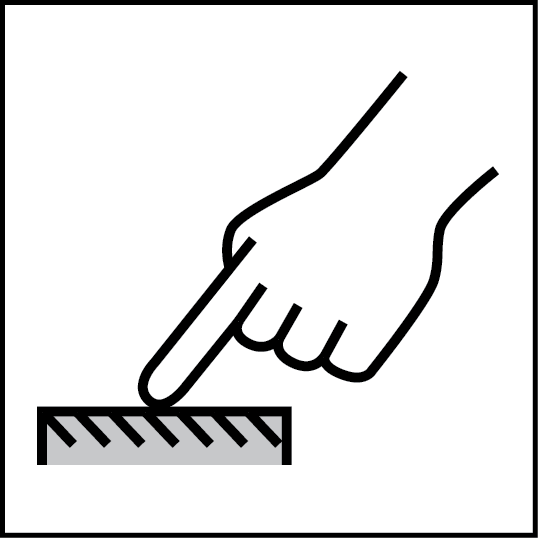
\includegraphics[height=0.3in]{figures/HapticExperienceLogo}
        %   & \textbf{Haptic Experiences}
        %   & \\
          
          \textbf{Code} & \textbf{Sub-theme descriptor} & \textbf{Explanation} \\
          \midrule
          \textbf{Co1}
            & %\textit{``Changes are to the guts''}
            Internal roles are interdisciplinary
            & It takes a multidisciplinary team to create a haptic design. \\ \midrule
            
            \textbf{Co2}
            &% \textit{``Have that solid click''}
            Engineering support
            & Prototyping is necessary and often delegated to engineers. \\ \midrule
            
            \textbf{Co3}
            & %\textit{``A reliable clock''}
            External roles are international
            & Haptic design teams work with other stakeholders around the world. \\ \midrule
            
            \textbf{Co4}
            & %\textit{``Feelable but not seeable''}
            Facillitators and advocates
            & Sales reps handle demos and fight for a deal. \\ \midrule
            
            \textbf{Co5}
            & %\textit{``Very individual''}
            Demos and documentation
            & Designers often show instead of telling. \\
        
          %\bottomrule
      \end{tabular}}
    \end{table}


\subsubsection{\textbf{[Theme Co]} Collaboration: ``Rally the ecosystem''}
\label{sec:interviews:collaboration}
\noindent
In this section, we describe the collaborative ecosystem.
First, we provide an overview of group structure and interdisciplinary roles found in our participants' groups (Sub-theme Co1), including a focus on the role of engineering (Co2).
We then discuss the dispersion of stakeholders internationally and in different organizations (Co3), including a focus on the connecting role of sales representatives, %  a connecting role, sales reps (Co4), 
and the use of demos and documentation (Co5).
We distinguish the Collaboration theme (Section~\ref{sec:interviews:collaboration}) from the Cultural Context theme (Section~\ref{sec:interviews:culture}) by focusing on specific communication methods and roles rather than underlying values and widespread public consciousness.

\begin{table}[tbp]
    % \scriptsize
    \footnotesize
    \centering
    \caption{Internal roles, the various descriptors used to label them, and descriptions. Roles were grouped and named by the authors based on participant-provided descriptors.
   % \kmC{07.22: clarify who assigns these labels - author/researcher, or the designer interviewees? UX and Design will seem oddly named to many readers.}
    %
    }
    \label{tab:roles:internal}
    \fcolorbox{black}{lightgray}{
    \begin{tabular}{p{0.5in}p{1.1in}p{2.75in}}
         \textbf{Role}%/Division 
            &  \textbf{Descriptors} %terms %labels
            & \textbf{Description} \\ 
            \toprule
         UX
            & User division (P6), \newline
            User research (P5), \newline
           Ergonomics (P6), \newline
           Human factors (P1), \newline
           Psychologist (P2,6)
            & The UX team does research: \qterm{P5}{facilitate prototypes, validate, communicate those results}.
            Here we include psychologists and human factors roles because they conduct user research such as evaluation:
            \qterm{P6}{psychologists there who do usability tests},
            %, may have electrical engineers too
            \qterm{P1}{study how effectively how users interact w/ goals}.
            %first job w/ air force.
            % & P6: \#s of people doing analysis, etc. psychologists there who do usability tests, may have electrical engineers too (related to science/UX?). P1: usually how effectively how users interact w/ goals; first job w/ air force. important in the world, what they pay attention to. don't know what's import. interesting analyzing real-world streams; underlying perceptual dimensions are all similar. work in GE global design; improve comfort and differentiate based on branding (if only compete on cost; then this is tough) (P1) \\ \midrule
            \\ \midrule
        Design 
            & Design team (P5) 
            & Related to UX but a separate and in some ways higher-level role. The design group ideates and communicates vision, developing a value proposition. Designers usually have a similar background to the UX group (P5).
            \\ \midrule
        
        
        Engineering 
            &
            Tech manager (P3), \newline
            Engineering (P3,5) \newline
            Electronics, mechanics, tech team (P6) \newline
            & Often a separate division, handling prototyping and implementation (P5).
            They might test components, do %everything to do with
            physical construction, take requirements from design, ergonomics, electronics, mechanics, etc. and generate required (haptic) feedback (P6).
            This can involve both hardware and software.
            \\ %\bottomrule
      \end{tabular}}
    \end{table}
    
All six participants indicated collaboration was an important part of their work and design process.
Haptic designers are part of interdisciplinary, international teams, and do not make haptic experiences alone:

\begin{quote}
    \qquote{P5}{We basically have to rally the ecosystem...we have to go and find, y'know, somebody to supply the amplifier part, somebody to make the motor, somebody who knows enough about the Android kernel...we have to be, kind of, renaissance men if you like}.
\end{quote}


\themeHeading{Co1}{``I'm not so much of a psychologist''}{Internal roles are interdisciplinary}
% \inlineHeading{Internal roles are interdisciplinary}
%Unsurprising given haptic technology's multimodal nature, h
Haptic design is interdisciplinary; hardware, software, psychology, and business all play a role.
%P1 mentions the influence of different roles/backgrounds, e.g., \qterm{P1}{technicians don't give pushback if they believe they have a problem}.
P5 describes his company's job as \qqquote{rallying the ecosystem}, finding diverse expertise and establishing a production chain.
P6 describes different roles in her team, who work more closely together at different stages: \qterm{P6}{user [research], design, ergonomics, haptics, electronics, all come together}.
This is reflected by the diverse internal roles (\autoref{tab:roles:internal}), but also in the diverse work in single projects and individuals:
% A single project can involves tasks from hardware to software and high-level design:

\begin{quote}
\qquote{P3}{We do some mechanical integration work, we help [our international customers] with designing the electronics, we have reference designs there, we have a couple of reference effects, and then we ship the part back and they go on with further doing the software integration and designing the haptic effects.}% that they want to have}.
\end{quote}

Our participants worked in groups of various sizes.
P2 worked with a student in a team of 2, while P5 describes several teams: design, UX, engineering, each with different responsibilities.
This collaboration can be collocated or remote: P6 describes the different divisions in her company as being physically close together, while P3 has sales representatives (\qqquote{reps}) overseas to help with external collaboration.

Especially in smaller groups, team members fill multiple roles.
Sometimes this falls naturally into their background:
%Even when a business model is software-focused, participants compare to physical domains:
\qquote{P5}{I guess [phone vibrations are] similar to mechanical control design, except that it's all virtual}.
Otherwise, this lack of expertise leads reduces confidence:
\qquote{P2}{I don't know, I'm not so much of a psychologist to really, to dare to say I can evaluate subjective responses to tactile feedback}.


%%quotes for interdisciplinary

% I don't know, I'm not so much of a psychologist to really, to dare to say I can evaluate subjective responses to tactile feedback P2

% we do some mechanical integration work, we help them with designing the electronics, we have reference designs there, we have a couple of reference effects, and uh, so  then we ship the part back and they go on with further doing the software integration and designing the haptic effects that they want to have P3

%I guess it's similar to mechanical control design, except that it's all virtual P5

% P6: We give them components to test; different phases. Need to know how to look, etc., layout needs to be done. very close physical location to team; know them well. Everything that has to do with physical construction. Take requirements from design, ergonomics, electronics, mechanics, etc. and make to generate the required haptic feedback. Have electrical engineers too


\themeHeading{Co2}{``Go through the technical levels''}{Engineering support}
% \inlineHeading{Engineering support}
Larger groups are able to have more specialized individuals.
Especially common was a dedicated engineering or technical support team, tasked with implementing prototypes for design and user research teams.


\begin{quote}
\qquote{P5}{In our design research team we don't do any internal prototyping, we rely on engineering resources to do all our prototyping}.
\end{quote}


P5's group says that neither the design team nor the UX team build prototypes, though the UX team facillitates and evaluates them. 
P1's team is similar:
\qterm{P1}{give qualitative feedback and ranges to the technicians}.
Engineering departments are sometimes \qterm{P6}{physically very close to other departments}, presumably to interact with different divisions and groups.
However, separating expertise can cause gulfs of collaboration, \eg, when P3 tries to propose a deal: 


\begin{quote}
\qquote{P3}{If you try to go through the technical levels from a technology scout to a technical manager and then maybe to a senior manager, you usually get blocked with something, 
%that, that you,
because nobody wants to take the risk or the blame}.
\end{quote}

\noindent
Those in engineering roles are risk-adverse:
\qquote{P3}{[it's] risky to suggest changes to their component}. %, so need to get around it}.
% Combined with the segmentation between engineering staff and the design or business group can lead to barriers, especially with respect to risk.
P3 says that to pitch to other companies, you need to reach \qqquote{C-level people} like the CEO, or other business or manager types:
%The members of the design and UX research teams have similar backgrounds (they are "fungible", except for preference for type of work); the trick is getting the right people to work together.
\qquote{P3}{engineers look at it from a perspective well I'm going to take a risk if I change something in my design, and if it doesn't work everybody's going to blame me},
\qterm{P1}{technicians won't give pushback if there is a problem}.
% This is most striking when trying to connect to business roles and other decision makers at other organizations.
%Have electrical engineers too, handles requests and gives support, physically very close to other depts., have electrical engineers (P6).
            % P5 describes his team \qqquote{engineering around} a software problem.
            % It's important to \qterm{P1}{always involve engineers, but they won't bring up issues always (no pushback if they see a problem)}
            % %Can be software (P5 had to engineer around API issues). Provide demos (P5) rather than design/UX team. P1: always involve engineers, but they won't bring up issues always (no pushback if they see a problem). P6: test components, do everything to do with physical construction, take requirements and generate required feedback. Note: designers are not engineers




\themeHeading{Co3}{``Different divisions, different companies''}{External roles are international}
% \inlineHeading{External roles -- connecting organizations internationally}
Haptic designers also worked closely with external stakeholders like potential customers and manufacturers.
%Our participants offered various products and services, such as actuators, the customization and installation of actuators, software, and designed haptic content.
Our designers have diverse suppliers, especially hardware suppliers, and often sell to manufacturers who then sell their own product to the end-user.
\autoref{tab:roles:external} provides details on these external-facing roles.

\begin{quote}
\qquote{P5}{Automotive is very much a tiered and compartmentalized manufacturing business, and so the person who makes the control surface is different than the person who makes the mounting for it...and those people often never talk to each other, and so for us it's even worse than different divisions in a company, it's different companies}.
%, um trying to get those people to talk to each other and to understand that haptics is a system-level solution that requires care and consideration at all these different levels, it's a whole different level of challenge}.
\end{quote}

Often these groups are distributed internationally.
P5's group, based in North America, received international demographics to research: \qquote{P5}{here's phone X from OEM Y and it's targeted at Asian ladies from 15 to 30 years old}.
P3, who has a headquarters in the North America and clients in Asia, describes \emph{sales reps} as critical team members who can bridge language and cultural barriers. %, and be physically present to run demos.
%P5: yeah, well, the bigger, I think the bigger problem is, haptics is a systems solution, it’s not a specific component you put in a system, so the motor is one of the biggest contributors, but so is the amplifier and the communication bandwidth between the amplifier and the CPU, and the CPU processing power for controlling the haptics, and the latency between the sensor and the CPU, all that stuff affects the experience and, unfortunately, each of those components is handled by a completely separate division of an OEM


%%quotes for stakeholders being spread out/disconnected
% “automotive has its own share of issues, we also do a ton of work in automotive, wherein for example for the Cadillac Q, that's our design, um   the, the challenge there is similar though I mean, automotive is very much a tiered and compartmentalized manufacturing business, and so the person who makes the control surface is different than the person who makes the mounting for it, right   it's different than the person that makes the board that controls the display, so and those people often never talk to each other   and so for us it's even worse than different divisions in a company, it's different companies, um trying to get those people to talk to each other and to understand that haptics is a system-level solution that requires care and consideration at all these different levels, it's a whole different level of challenge” P5

%and with a wide number of \textbf{stakeholders}, who are organized in 

%%quotes for international supply chain collaboration

    \begin{table}[htbp]
    \footnotesize
    \centering
    \caption{External roles, the various descriptors used to label them, and descriptions.}
    \label{tab:roles:external}
    \fcolorbox{black}{lightgray}{
    \begin{tabular}{p{0.5in}p{1in}p{2.75in}}
     \textbf{Role}%/Division 
            &  \textbf{Descriptors} %terms %labels
            & \textbf{Description} \\ \toprule
            
        Connections% \& sales
            & Sales rep, technology scout (P3) 
            & Sales reps from haptic companies handle local expertise (language and culture), haptics expertise (they run demos), and can be advocates for products. Technology scouts from large companies talk to haptics companies to learn their technology.
            \\ \midrule
        Business 
            &  Business dev people, % \newline 
            C-level people (P3) \newline
            & Internal business development people are \qquote{P3}{here [in HQ]}, while external business people make decisions; they're who you need to persuade, rather than technology-focused roles.
            \\ \midrule
        Supply chain 
            &  Vendor, developer, manufacturer, OEM % (original equipment manufacturer) 
            (P5), \newline
            supplier (P4,6), \newline
            content provider (P3) 
            & Haptic designers are heavily embedded in a supply chain involving hardware and software manufacturers.
            Some manufacturers provide hardware (e.g, actuators) and software (e.g., Android API) to the haptician, others are the intended customer (phone or car manufacturers, software developers).
            It is unclear who creates haptic content in this ecosystem.
            %
            % P5: Vendor (P5) – handset manufacturers, maybe this combines with OEM, Developer (P5) for software. 
            % %Manufacturer (also OEM??) (P5). OEM – original equipment manufacturer (P5), 
            % different divisions handle CPU, haptics, sensor, communication between them, want to put latest code from Google into handsets, also have tight fixed cost model
            % % OEM mentioned by other interviewees as well
            % Supplier (P4, P6) – is this also manufacturer?, NOT THE CUSTOMER it would seem
            % Content providers (P3): something they don't do, they need to get content creators interested, want to get into the emotional side of haptics
            \\ %\bottomrule
             \end{tabular}}
    \end{table}

\themeHeading{Co4}{``Sales reps''}{Facilitators and advocates}
% \inlineHeading{``Sales Reps'' -- Facilitators and Advocates}
P3 describes sales reps in-depth as key team members.
Sales reps are trained locally at headquarters in North America, then are sent to the customers'
area, often in countries like Korea, Japan, China, and Taiwan which have large consumer electronics and gaming markets.
It is important that they % They can 
speak the local language and understand the local culture; they also facilitate demos and persuade customers to pursue business with the designer's team. %, becoming an advocate for the product.
%They can make sure demos work, because they can be quite complicated.
% They are a key part of an international team, important for P3's US-based company reaching out to countries 
%, showing how to use the hardware (they've been trained), and creating or becoming advocates. 
If a demo is sent to a company without a sales rep, customers may respond by shipping the device back and requesting assistance, but often don't respond at all:

\begin{quote}
\qquote{P3}{If we try to just ship them a part...in the best case they come back and say well it doesn't work as we thought, can you help us?...in the worst case they don't even contact us back and we never learn why they didn't pursue an idea or an opportunity. It's still a complicated setup to make haptics work, there's lots of aspects that you have to take into account, and if you don't do it properly, you're going to be most likely very disappointed about what the outcome is}.
\end{quote}

%this can be very disappointing if you don't do haptics properly, it's very complicated to set up. 
%ship device mockups and evaluation kits back and forth;
%The relationship with other companies depends on whether they are big/small, what their project goals are; language, cultural, geographic differences, sales reps help with these and with demos, which *need to be done properly* or they're ineffective,
%In \autoref{tab:stakeholders}, we connect sales reps to another connecting role: tech scouts.
%and customers won't pursue an idea;

Big tech companies sometimes invert this from a push model (where the haptics company uses a sales rep) to a pull model with tech scouts (who reach out to haptics companies).
Sometimes, companies fill this role without dedicated sales reps: P4 goes to customers 
regularly in confidential meetings, receiving specifications and working collocated with the customer to get their product to feel \qqquote{just right}:


\begin{quote}
\qquote{P4}{There is always [the] option, as we did with one of our customers, that we simply went into the lab for a day or two, and just worked on simulated button feel, together with the customer, to get the feel just right}
\end{quote}

In all cases, content can fall through the cracks. 
P3's company provides technology, but \qquote{P3}{the issue that we are having with uh, the content providers that need to get interested and believe in % into %SLC: OS 07.26 I believe the participant says "believe into it", but it could also be "belief into it" or something. the "into" is not very clear so it's possible that he says "in", and in any case it cleans up the quote without distorting the message so I think we're fine to go with "in"
it...creating the haptic effects is something that we haven't been involved in in a lot of detail in the past}.
P5's company does have a set of 150 effects, from which they select themes.
The other participants all mention technology they develop, with content directly related to their hardware solution.



\themeHeading{Co5}{``Your piezo demo, we love it''}{Demos and documentation}
% \inlineHeading{Demos and Documentation}
Demos are essential to showing both the value of a haptic experience and enabling two-way communication with the customer.
They can clarify requirements and grab attention from clients:
\qquote{P5}{we'll often get the OEMs who will say, well you showed us your piezo demo, and we love it, it feels great}.
Demos can be conducted in-person (synchronously) at events like tech-days or one-on-one meetings:
\qquote{P4}{the customer either comes directly to us, we go towards our customers regularly, have our tech days, similar to automotive clinics}, or asynchronously, remotely shipped.

However, demos are complicated and need an experienced handler like a sales rep.
%if try to just ship them a part, and a lot of them they are asking for it, well just ship us your part, we take care of integrating it ourselves, in the best case they come back and say well it doesn't as we thought can you help us, and they probably ship us back what they put together and we try to fix it in the worst case they don't even contact us back and we never learn why they didn't pursue an idea or an opportunity, cuz they, it's still a complicated setup to make haptics work
%\qquote{P3}{the sales rep knows how to operate it}.
Once set up, demos are often adjusted, but this is easier than the setup: % possibly needing extra demo infrastructure or an experience demoer:
\qquote{P4}{From the moment the actuation module was working...it was just cranking up the maximum current or reducing the maximum current}.


Demos are often collected into groups.
P5 describes downloading apps that use his technology and \qqquote{sticking those in [their] demo suite}.
P1 and P2 talk about collecting examples for inspiration and guidance early in design:
it's \qqterm{quicker to go out and buy examples}, like \qterm{P1}{15 or 16 appliances that had notably different feelings}.
P2 instructed his student to \qqquote{collect physical push buttons just to get in contact with all the diversity of stuff}, and ended up with a \qqquote{button board} to guide design.
He also talks about company guidelines:

\begin{quote}
    \qquote{P2}{When I was at [a major automotive company] 3 years ago...they had this guideline book...they had guidelines on the design of physical widgets like sliders, physical sliders, push buttons, rotary things...they defined thresholds basically where these forces have certain thresholds and if you get over the threshold something is happening}.
\end{quote}

Demo setups can thus be stored long term for internal documentation (button board, guideline book), but they can also be ephemeral (tech days).
% Rapid collaborative editing can be useful to find what feels right, especially when designers have to deviate significantly from a direct translation of mechanical button in order to be compelling.
% This often stems from customers not knowing what is available to them.
%:\qquote{P4}{we had one sample, the customer a surface acceleration of 10 to 20 G perpendicular and a travelling distance of 2-3 tenth of a mm, we ended with an acceleration of 2G and a travelling distance of .4 of a mm, so, due to the size of the module, simply the high accelerations were too high for a good variable feel of the module}.
%Demo kits can even be sent to potential customer so they can protect their intellectual property.
%\osC{todo: resolve this with next 1-2 sections}
In both cases, they can help to articulate the value, especially valuable when most people do not yet understand haptic technology.


%Button Board Quotes:
%P1: quicker to go out and buy examples. collect a bunch (15 or 16 appliances that had notably different feelings). ******
%I had the special? student of mine, and I know that he’s really into sketching hardware and building stuff and he is doing stuff with Arduino, so I asked him to collect physical push buttons just to get in contact with all the diversity of stuff P2
%we made this button board, we called the thing a button board and it was a, (incomprehensible) button board, and we tried to implement as much different push buttons as we could find in this um, in this board P2
%when I was at (company) 3 (incomprehensible) years ago they had this, yeah, it was like, a guideline book, they had this guideline book on physical push buttons, so they defined, redefined the forces that are needed to make a push button a (incomprehensible) push button
% so they had guidelines on the design of physical widgets like sliders, physical sliders, push buttons, rotary things, this was really interesting P2
% mm, yeah, these (company) design guidelines they’re really basic, and they had all these different kinds of buttons like push buttons with two states, or push buttons with only one state and you, can release it again, and they defined thresholds basically where the forces, these forces have certain thresholds and if you get over the threshold something is happening so  um, I think this is much more a design thing to, to coin a trademark or something (P2)

%P5 demo suite quotes:
%and so, I think the most memorable day was when we started downloading apps, and realized that, yes, in fact this does work, and not only does it work but it works pretty well for a variety of apps, and it was a couple of surprising apps that it worked really well for, and basically we ended up just sticking those in our demo suite even though we had no relationship whatsoever to the developer  so, their app just worked, and it worked really well. P5
%P5: right. and, we’ll often get the OEMs who will say, well you showed us your piezo demo, and we love it, it feels great, we’re building this phone that has a, y’know, 10 cent eccentric mass motor in it, can you make it feel the same? Right, and the answer of course is no.


%%quotes for setting up/operating demos, setups
% •	“from the moment the actuation module was working, it was uh, not much of a scaling factor, it was just cranking up the maximum current or reducing the maximum current.” P4 (note – also need to customize/tailor)
%P3: if we um, try to just ship them a part, and a lot of them they are asking for it, well just ship us your part, we take care of integrating it ourselves, in the best case they come back and say well it doesn't as we thought can you help us, and they probably ship us back what they put together and we try to fix it in the worst case they don't even contact us back and we never learn why they didn't pursue an idea or an opportunity, cuz they, it's still a complicated setup to make haptics work

% \osC{TODO: move this vignette elsewhere, maybe to iteration?}


%%%%%%%%%%%%%%%%%%%%%
% Subsection: Cost/benefit not clear
%%%%%%%%%%%%%%%%%%%%%
\subsubsection{\textbf{[Theme CC]} Cultural Context: ``A standard feature, in the future''}
% \subsection{Cultural context: ``It is too new''}
\label{sec:interviews:culture}
%of haptics is not yet persuasive}
\noindent Haptic technology has yet to fully penetrate the public consciousness.
Participants reported major difficulty when working with both customers 
and users, including a limited understanding of what haptic technology is and how to work with it: %, partially because of the youth of the field.

\begin{table}[htbp]
    % \scriptsize
    \footnotesize
    \centering
    \caption{Sub-theme summaries for the Cultural Context (CC) theme.}
    \label{tab:experience:cultural:overview}
    \fcolorbox{black}{lightgray}{
    % \begin{tabular}{p{0.03\textwidth} p{0.33\textwidth}p{0.55\textwidth}}
    \begin{tabular}{p{0.05\textwidth}p{0.37\textwidth}p{0.45\textwidth}}
        %   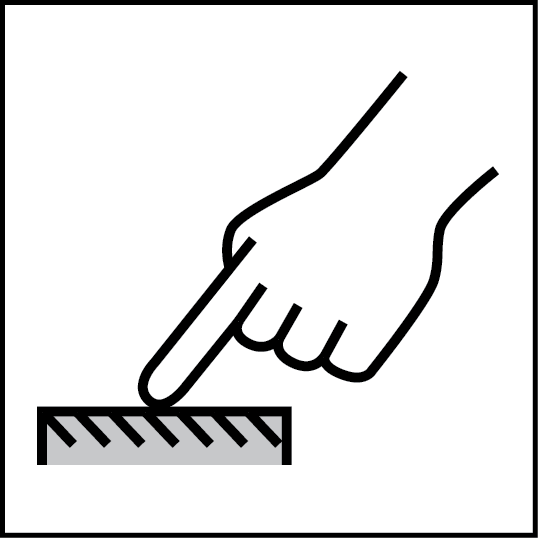
\includegraphics[height=0.3in]{figures/HapticExperienceLogo}
        %   & \textbf{Haptic Experiences}
        %   & \\
          
          \textbf{Code} & \textbf{Sub-theme descriptor} & \textbf{Explanation} \\
          \midrule
          \textbf{CC1}
            & %\textit{``Changes are to the guts''}
            Understanding requirements
            & Customers and designers have trouble articulating and understanding goals. \\ \midrule
            
            \textbf{CC2}
            &% \textit{``Have that solid click''}
           Evaluation
            & Getting experiences to feel right, usually with acceptance testing and deployment. \\ \midrule
            
            \textbf{CC3}
            & %\textit{``A reliable clock''}
            Secrecy and intellectual property
            & Haptic technology and sourced components are often cutting edge and secret. \\ \midrule
            
            \textbf{CC4}
            & %\textit{``Feelable but not seeable"}
            UX and branding
            & Tactile experiences provide intangible benefits. \\ \midrule
            
            \textbf{CC5}
            & %\textit{``Very individual"}
            Overcoming risk and cost
            & Haptics are risky and expensive to include in a product. \\
        
          %\bottomrule
      \end{tabular}}
    \end{table}

% \begin{quote}
%     \qquote{P3}{It's a little bit like with uh, the gyroscope sensors, in the beginning they were kind of using this just to change the orientation from landscape to portrait on the mobile phone...and then somebody came up and used it for games and today it’s used for navigation and all kinds of things, uh, so I think [haptic] technology today is really at an early stage, when you compare it to graphics, uh, it might be 30 years behind graphics, or maybe I'm too pessimistic there}.
% \end{quote}




\begin{quote}
    \qquote{P3}{People really don't know what to do with [haptics] and I think within the haptics community we need to...continue to push it into the market, but once it's there I think it's going to add to the user experience and will be a standard feature in the future}.
\end{quote}


Specifically mentioned were the difficulty in understanding customer requirements (CC1), and knowing how to appropriately evaluate haptic experiences (CC2).
As a technological field, secrecy and intellectual property are important concerns for both designers and customers (CC3).
Designers had ways to pitch the value proposition of haptics, often tied to UX and branding (CC4), but risk and cost of adopting the technology often make it a hard sell (CC5).


\themeHeading{CC1}{``Hard to express what they need''}{Understanding requirements}
% \inlineHeading{``Hard for them to really express what they need'' -- Understanding requirements}
\label{sec:interviews:express}
%: Language, content, and requirements}
Customers found it difficult to both understand and request their needs.
Our participants focused on the end result because it gives them and their colleagues the ability to solve problems: \qterm{P6}{Don't specify elements. Only give end product. Don't tell how to restrict; can give hints}.
However, requested end-results are often vague or confusing, like \qquote{P4}{good variable feel}:

\begin{quote}
    \qquote{P4}{The customer only came with a question, yeah, how [can the design] feel variable? Here it did not really describe how it should feel variable}.
    %, that was the most important question he had}.
\end{quote}
% \kmC{07.22: confusing. is 'customer' 'it'? is customer asking to be taught how to make it feel variable, or describing requirements?}

To make these impressions concrete, customers initially give engineering parameters as their best guess.
P4 in particular talks about his customers, who might point to a \qqquote{reference button which is available directly on the market, from companies like [company 1] or [company 2], and they say it has to feel exactly like this button}, or
request \qquote{P4}{a surface acceleration of 10 to 20 G perpendicular and a travelling distance of .2-.3 mm}.
This might have little relation to the final result, after the designers iterate with the customer: \qquote{P4}{we ended with an acceleration of 2G and a travelling distance of .4 of a mm, so, due to the size of the module, simply the high accelerations were too high for a good variable feel}.
The goal function of good variable feel was achieved, but the initial engineering-level specification was completely off.

% two different ways: low-level engineering parameters like \qterm{P2}{force profiles} or \qterm{P4}{travel distance} and high-level affective terms like \qterm{P2}{feeling right or alive} or \qquote{P4}{good variable feel}. 
% Examples, such as physical reference buttons, are used for requirement expression from clients, communication between and within organizations, and ideation.



% P4: hm. (incomprehensible) there is always option, as we did with one of our customers, that we simply went into the lab for a day or two, and just worked on simulated button feel, together with the customer, to get the feel just right so, we modified the push(?) strength, the push profile, so the actuator profile, we modified the damping, the spring constant, the spring behaviour, of our actuator, similar as you would do it on a mechanical button, and really tested for hours(?) several different versions of it, using Mickey Mouse ears

% \begin{quote}
%     \qquote{P4}{Because tactile feedback technology is so new, also for them it is too new, so, it's hard for them to really express what they need}.
% \end{quote}

Other participants showed this duality between high-level affective goals and low-level guesses.
P1 especially used affective and psychological terms when considering design, such as semantic differential scales:
\qterm{P1}{good/bad; gender (robust/delicate; size); intensity (sharp/dull; bright/dim, fast/slow); novelty}.
Haptic designers often connected low-level/high-level terms through iteration, or with their own way of representing features like quality:
%\qquote{P5}{solid click at 150 plus some audio at 300 or 400 Hz, which is going to give you that sense of quality, and, consistency across the whole dashboard},
\qquote{P5}{[audio click gives] quality, and, consistency across the whole dashboard},
\qterm{P6}{mass is big for quality...for the haptics, nice feedback w/ good snap gives a sense of quality}.
% Our designers must pay attention to these details: \qquote{P6}{Take into account fashion and consumer electronics; what does one associate with quality. Let this influence.}




% P4: it’s, because it’s uh, tactile feedback technology is so new, also for them it is too new, so, it’s hard for them to really express what they need



%P3: P3: well, um, that is the uh, the issue that we are having with uh, the content providers that need to get interested and believe into it, so we are providing the technology that allows and enables to create high-definition feels over a very broad frequency range, with enough strength and small enough, and especially very fast response time, so that’s our business now creating the haptic effects is something that we, we haven’t been involved in in a lot of detail in the past and that’s why I, I actually contacted Karon to help us with that and uh do a study and start working also on the emotional side of haptics but, that’s something that, we haven’t done a lot 
%P3: people really don’t know what to do with it and I think within the haptics community we need to make sure that we don’t lose our breadth and have enough um, kind of resources to continue to at the moment rather push it into the market, but once it’s there I think it’s, it’s going to be, going to add to the user experience and will be a standard feature in the future, it’s like like having a touchscreen now on smartphones which nobody expects any other way anymore uh, it’s just, I mean it happens to me that I sometimes pull out my old, uh, tom-tom navigation device in my car and I, I uh, and that one didn’t have a touch screen back then (laughing) so I tap on that one and so it’s the same thing with haptics, at some point it’s just going to expect that you get some nice haptic feedback and uh, but uh getting there is still a couple of years out, so, I think


%P3: P3: um, yeah, I would say it’s a little bit like with uh, the gyroscope sensors, in the beginning they were kind of using this just to change the orientation from landscape to portrait on the mobile phone and then they kind of put in that rather extensive sensor back then for uh, a limited functionality and then somebody came up and used it for games and today it’s used for navigation and all kinds of things, uh, so I think the technology today is, is really at an early stage, it’s probably when you compare it to graphics, uh, it might be 30 years behind graphics, or maybe I’m too pessimistic there but


%P4: P4: uh, that’s, different. Some customers say, there’s a reference button which is available directly on the market, from companies like ??? or ???, and they say it has to feel exactly like this button (laughing) I’ll just say, yes, we expect the surface movement or, there’s an acceleration of 10G, for example, and a, there’s a movement distance of 1/10th of a millimetre, and try to just describe the physical movement of the button, or of the touch pad.

%P6: Mass is big for quality; surface temp. (no metal); optics for surface. For the haptics, nice feedback w/ good snap gives a sense of quality. A good negative torque with encoder.
%P1: Caution against novelty because this will wear off; focus on everything else instead. Chasing new designs. Novelty was associated w/ an usual sound; uniqueness was good.
%P1: novelty is also an emotional dimension. can get emotion bang for buck w/ novelty.
%NOTE: P1 used more psych terms than low-level engineering or physical params
%p1: - use psychology techniques:  semantic differential method (rating scale of two opposite words) -- sound or tactile control
%- a number of word pairs. not too narrow on a particular experience
%P1: - pattern:  always same 3 clusters of words:  (SEMANTIC DIFFERENTIAL)
    %  good / bad; 
    %  gender; (robust/delicate; size; small) -- not +ve / -ve
    %  intensity; (sharp / dull; bright/dim; fast/slow);
    %  novelty (Jim's own experience; applied find); sony -- dominance? (consumer products)
% %P1: 4 dimensions equal? some are more prominent; some shifting occurs. use factor analytics techniques; clustering of variance is explained & hierarchy; good / bad is usually 1st or 2nd most important. most interesting are the others that get into subtlties.
% controls usually have a robust vs. pliable feel. Intensity in detents; esp. knobs or buttons.
    % - think of 2 criteria (word pairs to describe these dimensions).
    % - depending on product, choose words for a product. words are targeted w/ conveying info.
    % - e.g., feminine brand image.
    % - Art:get a sense of the subtlties.



% - different urgency differed in terms.


\themeHeading{CC2}{``It feels right''}{Evaluation}
% \inlineHeading{Evaluation}
Our designers all evaluated their designs but demonstrated different methods of evaluation, consistent with our workshop survey (Section~\ref{sec:workshop}).
P2 explicitly evaluates both low-level, pragmatic concerns (\eg, task accuracy and speed) and high-level affective concerns like feeling personally involved (with the AttrakDiff questionnaire~\citep{Hassenzahl2003}, \url{http://attrakdiff.de}).
P5's user experience team conducts validation (but was unable to share details). %(details aren't included).
Small-scale acceptance testing was employed by both P2 and P4: when iterating in-person with the customer, P4 kept iterating until the customer said it \qqquote{felt right}; P2 only had himself and his student evaluate their designs in an academic context, despite indicating a desire to do a more thorough evaluation.
P3's group doesn't create content, but indicated a desire to look into that and investigate it with studies.


% There seems to be 
Our participants expressed a clear desire for stronger evaluation, but reported %the present reality is % as-is, it's 
mostly lightweight, \emph{ad-hoc} acceptance testing. 
This is consistent with our workshop findings, which suggest little real-world or \emph{in situ} evaluation. 
One reason may be that evaluation tools need to be adapted. P2 describes having to \qqquote{throw out} terms on the AttrakDiff questionnaire that did not fit, and iterate on the questionnaire.
%\kmC{07.22: WHY? need to dig deeper here.}
% (P1, P6??)
However, deployment seems to be a natural way to see if the design is good enough, as the ultimate acceptance test.
P5 described the most memorable moment of his software project being when his product had been deployed and used by a software development team.
Seeing a haptic-enabled app available for download, and feeling it in context, was impressive:

\begin{quote}
    \qquote{P5}{I think the most memorable day was when we started downloading apps, and realized that, yes, in fact this does work, and not only does it work but it works pretty well for a variety of apps...
    %, and it was a couple of surprising apps that it worked really well for, and basically
    we ended up just sticking those in our demo suite even though we had no relationship whatsoever to the developer. So, their app just worked, and it worked really well}
\end{quote}



\themeHeading{CC3}{``Kept confidential''}{Secrecy and intellectual property}
% \inlineHeading{Secrecy and Intellectual Property}
\label{sec:interviews:culture:secrecy}
%When establishing requirements, designers work closely with clients, with back and forth to understand their goals:
%\qquote{P4}{the customer only came with a question, yeah, how does it feel variable? (laughing) here it did not really describe how it should feel variable}.
Sometimes the customer does not know what they want, but in other cases, they have important information they need to withhold.
%Like many fields of technology, haptics is no stranger to confidentiality.
%in high-tech companies, like haptics.
As mentioned in Section~\ref{sec:interviews:experience}/Ex4, secrecy in haptics has major implications that inhibit design, especially given the verticality of haptic technology:

\begin{quote}
    \qquote{P3}{Somebody wants to design a completely new gaming controller for a gaming console, so they might just have some CAD drawings or they might have something they don't want to share with us, so in that case we provide them an evaluation kit...we don't need to know what their design looks like, they can really work on it internally}
\end{quote}

P3's clients are able to receive an \qqterm{evaluation kit} and create content with audio editors.
P4 describes meetings with customers that preserve confidentiality:
%and tech days, where just customer, themselves, and \qqquote{not many suppliers} are present, to preserve confidentiality.
\qquote{P4}{on these tech days it's usually only one customer and not that many suppliers at the same time, sometimes only the customer and us, to make sure our development is kept confidential}.
Once technology of P4's company is on the market, it is no longer secret - rivals can copy or reverse-engineer the devices, so there are many demonstrations to customers before release of the tech.
P4 wants to show their technology to potential buyers, not competitors. %\kmC{07.22: clarify causality in preceding sentence. How do 'many demos' help this situation?}


Secrecy can cause delays for software too.
P5 delivers a modified Android kernel to his customers, who are software developers.
However, they are not given an early release, and thus they \qquote{P5}{always lag the market by two months at least, to get an update [for Android]...it's annoying because, you know, as soon as the OEMs get the source code they want to put it in their product right away}.
%, and then we say, but just wait, it’ll take us a couple months to do it.}
%So secrets are kept both in the haptics company and in the client's - in the client's case, essential components like the final visual design are kept secret *****, critical in such a multi-factored, vertical industry.
% Because haptic technology is not directly supported in the software pipeline, customers (in this case, software developers) are forced to wait.

% P4: we cannot really keep our technology itself confidential, that’s uh, that’s at least as soon as a product is on the market, our competitors take the product and disassemble it, so they know about our technology, and therefore we of course try to present our technology before we get it into the market.
% P4: the design processis not really that, that much of our own intellectual property only, so that’s always, in discussion with the customer and together with the customer and uh, the customer is dealing with our competitors as well, so they are using the same technologies and designing it, but uh, the, technology behind this interface (are fixed?), that was uh, what the end customer does not see, that’s certainly our own technology. that’s, that’s kept confidential until the product is on the market. But I’m not sure that was your real question. (laughing)


%%quotes for specifying and understanding goals
% \osC{are these quotes handled effectively already?}
% Because it's hardware, they cannot keep their designs confidential \qquote{P4}{as soon as a product is on the market, our competitors take the product and disassemble it, so they know about our technology, and therefore we of course try to present our technology before we get it into the market}.
% \qquote{P4}{and on these tech days it's usually only one customer and not that many suppliers(?) at the same time, sometimes only the customer and us, to make sure our development are kept confidential}.
% \qquote{P5}{I think the, the other thing which is sort of challenging is that uh, Google doesn't give out source code until after the product is released, and so we always lag the market by two months at least}.









\themeHeading{CC4}{``Articulating the value''}{UX and branding}
% \inlineHeading{``Articulating the value'': UX and branding}
\label{sec:interviews:value}
Our participants were all passionate about haptic technology and its benefits.
The value of haptics can be connected to better performance on various tasks: P2 tried to \qqquote{support people interacting bimanually to find out if they are more accurate in drag and drop tasks, [or] faster}, but also whether they would \qquote{P2}{feel more personally involved in the interaction somehow}.
This latter goal, of user experience or rich feedback, was the primary value for haptics:

\begin{quote}
    \qquote{P3}{It's like having a touchscreen now on smartphones which nobody expects any other way anymore...sometimes pull out my old, uh, tom-tom navigation device in my car, and that one didn't have a touch screen back then (P3 laughs) so I tap on that one [expecting it to respond to touch input], and so it's the same thing with haptics, at some point it's just going to expect that you get some nice haptic feedback, but getting there is still a couple of years out}
\end{quote}
% \kmC{07.22: note, 'a couple years out' said in 201\osE{2}. Remark on this?}

\noindent 
Of course, \qqquote{a couple years out} has already gone by as of the time of this writing; and indeed, haptic feedback is now normal and expected in many touchscreen products, although quality and range continue to be challenging.

As mentioned in \autoref{sec:tailoringandcustomization}, tailoring and customization are important for each implementation.
This is also true for value:
differentiable sensations are important to help distinguish overall user experience and provide branding.
\qterm{P1}{look for alarms that were different; branding.effective, but different.}.
Companies and products need to have both a cohesive and differentiable feel.
P2's company \qqquote{guideline book}, which defined force profiles for buttons, was helpful to \qquote{P2}{coin a trademark}.
%P2 and his student follow this book but contrast it with their ``button box'' of examples to help find compelling, but consistent, force profiles.

\begin{quote}
    \qquote{P5}{[We] provide differentiated tactile experiences to our customers, who are major mobile phone manufacturers. Since Android is pretty generic across the board, um, they like to have custom themes, which are sets of these 150 effects}.
\end{quote}

\noindent With software libraries, themes are essential to the haptic design process.
This desire for consistent output has a tension with customization and fine-tuning:
\qquote{P5}{it's also important to tune the experience depending on whatever kind of motor they decide to put in}.
% \qterm{P1}{look for alarms that were different; branding. effective, but different.}
This is part of the the persuasive capability of touch:
\qterm{P6}{improve comfort and differentiate based on branding}. % (if only compete on cost; then this is tough)}.





\themeHeading{CC5}{``A tough sell''}{Overcoming risk and cost}
% \inlineHeading{``A tough sell'' -- Overcoming risk and cost}
Despite its value, haptic technology is a risky, costly feature to add.
Providing improved user experience requires \qqquote{high-definition haptics}, not \qquote{P3}{some rumble feedback that has been around a long time}.
This often means \qqquote{going up in fidelity} from a \qquote{P5}{cheap, poor quality motor}.
P5's company argues that \qqquote{the end-user is going to prefer this quality of experience} with improved hardware, like a piezo actuator.

\begin{quote}
    \qquote{P5}{[If we were to perform this project again,] I think we would spend a bit more time up front articulating the value, the specific value prop, of individual features}.
\end{quote}


\noindent P5 notes the challenge of convincing non-end-users to buy or deploy their technology:
\qquote{P5}{[our company] has the unique challenge that our customers are not the people who use our products}.
Since the main benefit is to the end-user's experience, % UX, 
it is challenging to connect to the bottom line, especially compared to other haptics components.
According to P3, designers need to

\begin{quote}
    \qquote{P3}{...get up to the decision-making level and more on the business side...[business roles] know nothing about technology, I mean, they don't care, but we are trying to demo parts to them, present business cases to them, and show them what they can do in order to gain market share, or increase their retail price when they add our technology}.
\end{quote}

%\kbC{ADDRESSED -- There are funny characters after the comma after ``gain market share'' in the source for the above quote.}
%\kmC{ADDRESSED -- 07.23: odd to have a long inline quote from P3, immediately followed by a separated P3 quote. Both quotes are valuable, and not redundant; can they be framed with your text more?}
%\kbC{ADDRESSED -- I broke the first quote from P3 out into a displayed quote.}

\noindent P3 further commented on lack of knowledge among dicison makers about haptics compared to other technologies.

\begin{quote}
    \qquote{P3}{Let's assume we were to work on a completely different product like memory chips, so everybody understands what this is for, what it can do, and you probably have a memory chip that is faster or, whatever, smaller. Now for haptics, this approach is kind of difficult because the technology scouts themselves they kind of understand what this is for, but how it it's going to add value to their device, and how much they can increase the retail price, or if they can increase it at all, or gain market share, that's completely open}.
\end{quote}






% \qquote{P3}{I think the technology today is, is really at an early stage, it's probably when you compare it to graphics, uh, it might be 30 years behind graphics, or maybe I'm too pessimistic there but  but that is still really new}

Newer technologies are hard to explain: \qquote{P5}{[Gesture-based haptic feedback is] a much more complex task to design, and also to explain, to the OEM}.
It can also make persuading a customer difficult.
%, because they are more concerned with the bottom line.
P3 finds that  \qqquote{there's always discussions on the cost}, and proposes
\qqquote{alternative business models} to no avail. % like contracts \qquote{P3}{you pay over two years for your phone}, they all fail.
Cost concerns are perfectly captured by P5:

\begin{quote}
\qquote{P5}{[The customer says,] `we love [the piezo demo], it feels great, we're building this phone that has a 10 cent eccentric mass motor in it, can you make it feel the same?' The answer of course is no}.
\end{quote}
% \begin{quote}
%     \qquote{P5}{we'll often get the OEMs who will say, well you showed us your piezo demo, and we love it, it feels great, we're building this phone that has a, y'know, 10 cent eccentric mass motor in it, can you make it feel the same? Right, and the answer of course is no.}
% \end{quote}

P5 notes that \qqquote{cost pressures are pretty extreme}. Mobile phones in the US cost \qqquote{\$199 on contract, that's sort of a fixed price and you can add more features to the phone, but that just reduces the profit margin, right?}, so \qquote{P5}{the addition of haptic feedback technology...can be a tough sell}.
Haptic technology is especially risky because of previously discussed challenges: it involves separate risk-adverse engineering divisions, and changes to the \qqquote{guts} of a product.
Designers need to set up complicated demos to persuade decision makers of the value of improved user experience: 
\qterm{P1}{if only compete on cost; then this is tough}.
Of course, \qqquote{it's hard to get through to the right level}, like \qquote{P3}{C-level kind of persons, so, talking to the CTO of Sony, those kinds of people}.
The combination of high-risk, increased cost, and indirect connection to the bottom line make haptics a very tough sell indeed.


%P3:  now in some companies that works well in other companies uh, you, it’s hard to get through to the right level, I mean, I’m talking about c-level kind of persons, so, talking to the CTO of Sony, to those kinds of people, those are the people that can really make a difference and say well, you guys work on this or you don’t if you try to go through the technical levels from a technology scout to a technical manager and then maybe to a senior manager, you usually get blocked with something that, that you, because nobody wants to take the risk or the blame if it’s not as good as they think, and uh, also they don’t have the business view, the engineers look at it from a perspective well I’m going to take a risk if I change something in my design, and if it doesn’t work everybody’s going to blame me so why should I do this, unless somebody tells me to do it, I’m not going to do it. So, that’s basically the situation




% \qquote{P3}{Now um when you, let's assume we were to work on a completely different product like memory chips or so everybody understands what this is for, what it can do, and you probably have a memory chip that is faster or, whatever, smaller, um now for haptics, this approach is kind of difficult because the technology scouts themselves they kind of understand what this is for, but how it it's going to add value to their device, and how much they can increase the retail price, or if they can increase it at all, or gain market share, that's completely open because haptics is still, well let's say high-definition haptics, I'm not talking about some rumble feedback that has been around a long time um}
% \qquote{P3}{yeah, yeah they, um, they are mainly looking after having better graphics and faster graphics, on-line capabilities, and adding sort of a hardware feature to their device in the beginning is mainly adding cost to it, and uh they have to go over uh, get over that hurdle to know whether the cost can be justified by the better user experience, and uh, as long as the content is not created, that is hard to do}

% \qquote{P3}{we are trying to demo parts to them, present business cases to them, and uh show them what they can do in order to gain market share, uh or increase their retail price when they add our technology}


%However, this can pose a barrier - the customer is not the end-user, but rather the manufacturer. P5's company has to balance both stakeholders, tricky when the main sell of haptics is the *user experience*.

%%quotes about risk, tech staff
% •	“also they are taking an additional risk because they are changing something through the hardware, it might not appear like that when you look into uh, the consumer electronics industry and you get the impression every other month they have a new phone or new, new kind of, new design, but the guts of it do not change much,  (laughing)” P3




%P1:  Human Factors -- usually how effectively how users interact w/ goals; first job w/ air force. important in the world, what they pay attention to. don't know what's import. interesting analyzing real-world streams; underlying perceptual dimensions are all similar. work in GE global design; improve comfort and differentiate based on branding (if only compete on cost; then this is tough).

%P3: people really don’t know what to do with it and I think within the haptics community we need to make sure that we don’t lose our breadth and have enough um, kind of resources to continue to at the moment rather push it into the market, but once it’s there I think it’s, it’s going to be, going to add to the user experience and will be a standard feature in the future, it’s like like having a touchscreen now on smartphones which nobody expects any other way anymore uh, it’s just, I mean it happens to me that I sometimes pull out my old, uh, tom-tom navigation device in my car and I, I uh, and that one didn’t have a touch screen back then (laughing) so I tap on that one and so it’s the same thing with haptics, at some point it’s just going to expect that you get some nice haptic feedback and uh, but uh getting there is still a couple of years out, so, I think

%P3: P3: um, so there’s the typical approach that uh, these big companies, like Samsung and Apple and HTC and Sony, where they are, their approach is to have technology scouts reaching out to you, and uh looking at your demos and then eventually kicking off a feasibility project. Now um when you, let’s assume we were to work on a completely different product like memory chips or so everybody understands what this is for, what it can do, and you probably have a memory chip that is faster or, whatever, smaller, um now for haptics, this approach is kind of difficult because the technology scouts themselves they kind of understand what this is for, but how it it’s going to add value to their device, and how much they can increase the retail price, or if they can increase it at all, or gain market share, that’s completely open because haptics is still, well let’s say high-definition haptics, I’m not talking about some rumble feedback that has been around a long time um  but that is still really new, and therefore, we are trying um, to rather get up to the decision making level and more on the business side, so those are people that are uh, to say it a little bit black and white, they know nothing about technology, I mean, they don’t care, but we are trying to demo parts to them, present business cases to them, and uh show them what they can do in order to gain market share, uh or increase their retail price when they add our technology

% P3: also they are taking an additional risk because they are changing something through the hardware, it might not appear like that when you look into uh, the consumer electronics industry and you get the impression every other month they have a new phone or new, new kind of, new design, but the guts of it do not change much,  (laughing) 
% P3: Now um when you, let’s assume we were to work on a completely different product like memory chips or so everybody understands what this is for, what it can do, and you probably have a memory chip that is faster or, whatever, smaller, um now for haptics, this approach is kind of difficult because the technology scouts themselves they kind of understand what this is for, but how it it’s going to add value to their device, and how much they can increase the retail price, or if they can increase it at all, or gain market share, that’s completely open because haptics is still, well let’s say high-definition haptics, I’m not talking about some rumble feedback that has been around a long time um but that is still really new, and therefore, we are trying um, to rather get up to the decision making level and more on the business side, so those are people that are uh, to say it a little bit black and white, they know nothing about technology, I mean, they don’t care, but we are trying to demo parts to them, present business cases to them, and uh show them what they can do in order to gain market share, uh or increase their retail price when they add our technology


%P5: yes, definitely. Yeah it’s a much more complex task to define- to design, and also to explain, um those to uh to the OEMs
%P5: yeah, um, let me see I think we would uh, spend a bit more time up front, articulating the value, the specific value prop, of um individual features, instead of, I would say the approach we took was more, hey it looks like we can do this and it looks like it’s interesting, so let’s do it right, which is kind of the engineering approach to product development, and I think, to do it again, wouldn’t require unlimited resources, it would require a bit more up-front time around thinking through where the best places to do this, and how can we best show that value, um in the user experience
%P5: P5: well, (company) has the unique challenge that our customers are not the people who use our products interviewer: yeah (laughing)  but, so there’s, yeah, so there’s medium and you have to meet the needs of both, I mean if you meet the needs of your, um, your front-line custom-, well your customers, then, their users, if they don’t like it then you’re going to have problems later on too
%P5: P5: sure. Well I mean, people building mobile phones are trying to, the cost pressures are pretty extreme, right, so, in the US most mobile phones that are high-end phones cost $199 on contract, that’s sort of a fixed price and you can add more features to the phone, but that just reduces the profit margin, right? and the purpose of the OEM, or their business model is to increase that margin as much as possible, while remaining competitive and so, the addition of haptic feedback technology is always, not always, but can be a tough sell, in terms of going up fidelity, for example. right? so we would argue to them that the end-user is going to prefer this quality of experience, um, if the additional cost to the bill of materials is significant, then that’s a tough argument to make, versus the OEM saying we’re just going to put this cheap, poor quality motor in the device, and it, you know, you get your vibration alerts when somebody calls, and that’s good enough, you know which from our perspective is not a sufficient end-user experience
%P5: P5: right. and, we’ll often get the OEMs who will say, well you showed us your piezo demo, and we love it, it feels great, we’re building this phone that has a, y’know, 10 cent eccentric mass motor in it, can you make it feel the same? Right, and the answer of course is no.
%P5: yeah, well, the bigger, I think the bigger problem is, haptics is a systems solution, it’s not a specific component you put in a system, so the motor is one of the biggest contributors, but so is the amplifier and the communication bandwidth between the amplifier and the CPU, and the CPU processing power for controlling the haptics, and the latency between the sensor and the CPU, all that stuff affects the experience and, unfortunately, each of those components is handled by a completely separate division of an OEM.

% P3: yeah, yeah, I mean, it would be, it would be sometimes discussion, I mean there’s always discussions on the cost, and we have been proposing also alternative business models but basically uh, that uh,  I mean, you can think about business models that are similar to like when you buy, when you sign up for a mobile phone or so where you don’t pay for the phone, it’s uh, or at least you don’t pay the total price, and you kind of sign up for a contract and so you pay over two years for your phone, we had kind of, that kind of proposal that would have been a bigger change but um, nobody really signed up for that one so



%P5: P5: sure. Well I mean, people building mobile phones are trying to, the cost pressures are pretty extreme, right, so, in the US most mobile phones that are high-end phones cost $199 on contract, that’s sort of a fixed price and you can add more features to the phone, but that just reduces the profit margin, right? and the purpose of the OEM, or their business model is to increase that margin as much as possible, while remaining competitive and so, the addition of haptic feedback technology is always, not always, but can be a tough sell, in terms of going up fidelity, for example. right? so we would argue to them that the end-user is going to prefer this quality of experience, um, if the additional cost to the bill of materials is significant, then that’s a tough argument to make, versus the OEM saying we’re just going to put this cheap, poor quality motor in the device, and it, you know, you get your vibration alerts when somebody calls, and that’s good enough, you know which from our perspective is not a sufficient end-user experience

%P5:  and actually what ended up happening is that, we moved all of that functionality into a different product line, um and so now the basic product just has what I would call static confirmation style haptic feedback, although it’s across a variety of locations in the UI, so maybe 120 or so different places where you have, you know, confirmation style haptics and then, we have a forthcoming product which will have all of the sort of dynamic haptic experiences, that are gesture driven
%P5: yes, definitely. Yeah it’s a much more complex task to define- to design, and also to explain, um those to uh to the OEMs
%P5: uh yeah, it’s a bit more complex for us, but the product actually, ships as a diff tree, to Android, so the customer just has to run a script um and it will patch all the changes into Android
%P5: P5: yeah, um, let me see, I think we would uh, spend a bit more time up front, articulating the value, the specific value prop, of um individual features, instead of, I would say the approach we took was more, hey it looks like we can do this and it looks like it’s interesting, so let’s do it right, which is kind of the engineering approach to product development, and I think, to do it again, wouldn’t require unlimited resources, it would require a bit more up-front time around thinking through where the best places to do this, and how can we best show that value, um in the user experience
%P5: P5: well, (company) has the unique challenge that our customers are not the people who use our products interviewer: yeah (laughing)  but, so there’s, yeah, so there’s medium and you have to meet the needs of both, I mean if you meet the needs of your, um, your front-line custom-, well your customers, then, their users, if they don’t like it then you’re going to have problems later on too


%P5: Oh sure, I mean you can make that argument, yeah, I mean, you can, you reduce cost, you reduce complexity, you reduce failure rates, all the stuff goes down, but the, the, problem in many cases is that the manufacturer doesn’t have the domain expertise or the process infrastructure to manufacture a haptic solution that’s, as compelling as a mechanical switch panel.



%P3: ideally you don’t even ship it back to them, you ship it back to your sales rep, and the sales rep knows how to operate it and goes back to the customer in a face-to-face meeting, shows it to them, and then they can take it from there, show it internally, especially when they go up the ranks, show it to a CTO or, that kind of person, that they actually become an advocate and feel comfortable with showing the prototype

%P3: P3: yeah, yeah they, um, they are mainly looking after having better graphics and faster graphics, on-line capabilities, and adding sort of a hardware feature to their device in the beginning is mainly adding cost to it, and uh they have to go over uh, get over that hurdle to know whether the cost can be justified by the better user experience, and uh, as long as the content is not created, that is hard to do





%%%%%%%%%%%%%%%%%%%%%%%%%%%%%


%QUOTES - Branding/Marketing



%P5:  and actually what ended up happening is that, we moved all of that functionality into a different product line, um and so now the basic product just has what I would call static confirmation style haptic feedback, although it’s across a variety of locations in the UI, so maybe 120 or so different places where you have, you know, confirmation style haptics and then, we have a forthcoming product which will have all of the sort of dynamic haptic experiences, that are gesture driven


%Haptics is New

% P4: we cannot really keep our technology itself confidential, that’s uh, that’s at least as soon as a product is on the market, our competitors take the product and disassemble it, so they know about our technology, and therefore we of course try to present our technology before we get it into the market.


            
            
% \begin{table}[ht]
%     \centering
%     \begin{tabular}{p{0.75in}p{1.5in}p{3.5in}}
%         \centering
%      Stakeholder%/Division 
%             &  Descriptors %terms %labels
%             & Description \\ \toprule
            
%         User
%             & Demographic (P5), [software] developers (P5)
%             & The end-user of the system, or participants used when studying the system. Can fall into targeted marget segments or demographics (\qquote{P5}{here's phone X from OEM Y and it's targeted at Asian ladies from 15 to 30 years old}), or people who use the software library (who have their own end-users).
%             Notably not customer for our participants.
%             %; the customer provides the user with haptics as part of their product.
%             \\ \midrule
        
%         Customer 
%             & Customer (P4, P5) 
%             & They can come to company or the company can go to customer (P4), sometimes just the customer is there (confidentiality).
%             Often has important systems knowledge they don't share (e.g., visual design, physical casing, other ``HMI'' data)
%             %and don't always share it;
%             Customers provide requirements and goal function, but it's hard for customers to express what they need. 
%             %P5: this is phone manufacturer in P5's case (OEM?) and maybe developers for P5? Not the user necessarily. o	User (P5,6) is not always customer
%             \\ \bottomrule
%     \end{tabular}
%     \caption{User vs. Customer \osC{todo: replace with figure?}.}
%     \label{tab:uservscustomer}
% \end{table}


% Haptics' benefit is unclear.
% (if only compete on cost; then this is tough) (P1)
% \qquote{P3}{once it's there I think it's, it's going to be, going to add to the user experience and will be a standard feature in the future}
% \qquote{P5}{I think the most memorable day was when we started downloading apps, and realized that, yes, in fact this does work, and not only does it work but it works pretty well for a variety of apps, and it was a couple of surprising apps that it worked really well for, and basically we ended up just sticking those in our demo suite even though we had no relationship whatsoever to the developer  so, their app just worked, and it worked really well}
%P3 on persuading people of haptics's benefits

%%Quotes for full UX
% •	“I think the most memorable day was when we started downloading apps, and realized that, yes, in fact this does work, and not only does it work but it works pretty well for a variety of apps, and it was a couple of surprising apps that it worked really well for, and basically we ended up just sticking those in our demo suite even though we had no relationship whatsoever to the developer  so, their app just worked, and it worked really well” P5

%%Quotes for user vs customer





%%%%%%%%%%%%%%%%%%%%%%%%%%%%%%%%%%%%%%
%
% Section: Workshop and Questionnaire
%
%%%%%%%%%%%%%%%%%%%%%%%%%%%%%%%%%%%%%%
%\section{Broad-Spectrum Follow-up: Workshop Findings}
\section{Part II: Validating the Findings in a Follow-Up Workshop}
\label{sec:workshop}
\noindent
\revOne{Our second study} was conducted during a workshop on haptic experience design at World Haptics 2015, the largest academic haptics conference, held that year in Chicago, IL, USA % a major academic haptics conference 
(\url{http://haptics2015.org}).
%\osC{TODO: link findings here to findings in previous section}

\subsection{Method}
\noindent
The workshop was organized by two of the authors % researchers  (the first and second co-authors)} % KM thinks we should not be identifying authors in this way.
% with the intent 
to initiate a conversation between researchers and industry practitioners about \haxd status and needs, and \\revOne{complement} our findings \revOne{from the first study by connecting with a broader set of hapticians}.

\subsubsection{Participants}
\noindent
Over thirty people participated in the workshop brainstorm session and the panel discussion.
Sixteen workshop participants responded to a questionnaire at the close of the workshop, which requested details about the respondents' roles, tools, and techniques. % (Section~\ref{app:questionnaire}).

Of 16 questionnaire respondents, 5 self-reported as working in industry, and the other 11 as members of academia (one  reported also working at ``other: research institute'').
For roles, 4 reported as graduate students, 4 as developers, 2 as designers, 2 as a combination of designer and developer, 2 as researchers, 1 as a business person (``product integration/commercialisation''), and 1 did not report.

\subsubsection{Procedure}
\noindent
Four leading haptic design experts -- two from industry, one academic and one with a foot in both worlds -- gave short \emph{presentations} on topics concerning both engineering and UX.
These presentations set the stage for a hands-on \emph{brainstorming session}, culminating in an audience-participation \emph{panel discussion} about challenges and ideas for \haxd. 
%\kmC{what about follow-up discussion?}
%\osC{Do you mean after the workshop? How it was received? Or the panel discussion itself, which included the general workshop participants? UPDATE: I think I've handled below?}

Brainstorming occurred in 6 groups of approximately 6-7 members.
Each group was asked to identify challenges faced by their members and then brainstorm solutions.
% , who tried to identify challenges faced by members of each group, then brainstorm solutions.
Brainstormed ideas informed the panel discussion, which was led by the four haptic design experts but included all workshop participants.
A questionnaire was distributed to all participants at the end of the workshop.
The questionnaire was supplemented with researcher notes written during and after the workshop, and the participant's sheets used for brainstorming, which were collected afterwards.

\subsection{Results}
\noindent
In the following, we report results from the questionnaire's quantitative and qualitative (open-ended) questions, along with findings from notes and brainstorming sheets.
%with the qualitative data gleaned from this venue -- open-ended questionnaire responses and themes from the brainstorming session and panel discussion, 
%\kmC{07.23: state how you collected data from the brainstorm and discussion, and what form it took - notes, live, videotaped - ??}

\begin{figure}[tb]
    \centering
    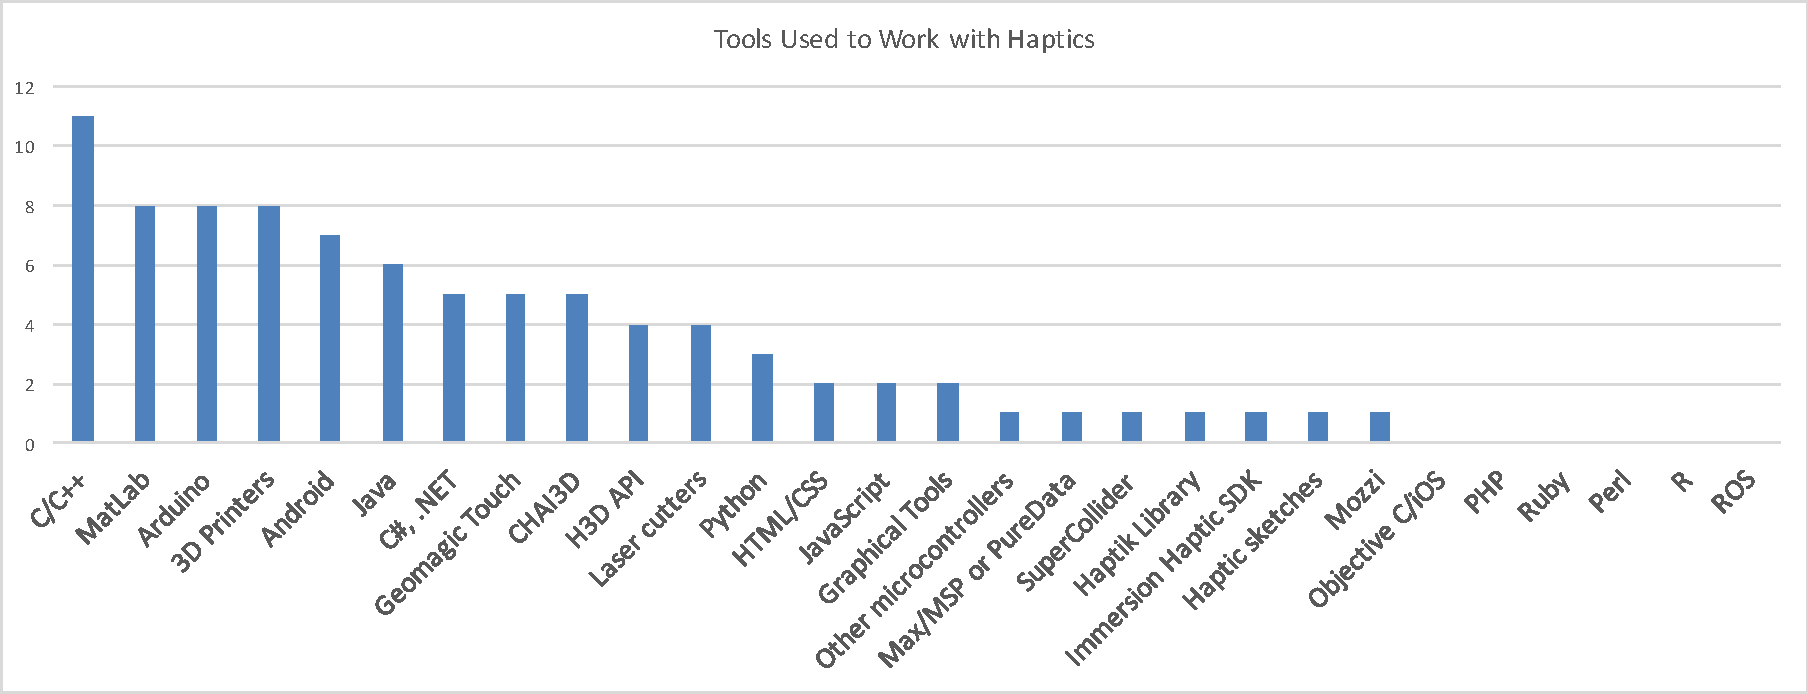
\includegraphics[width=\textwidth]{ToolResults-2016-06-29}
    \caption{Responses for tools used in haptic design (N=16, \emph{``check all that apply''}).}
    \label{fig:questionnaire:toolcounts}
\end{figure}

%%%%%%%%%%%%%%%%%%%%%
% Subsection: Quant Questionnaire Results
%%%%%%%%%%%%%%%%%%%%%
\subsubsection{Quantitative Data (survey): Tools, Background, Groupwork}
%
\noindent
Respondents reported a wide variety of hardware and software tools used to work with haptics (\autoref{fig:questionnaire:toolcounts}).
Most used were popular general or technical programming languages like C/C++, Matlab, Java, and hardware hacking tools like Arduino and 3D printers.
Force-feedback APIs for consumer hardware (Geomagic Touch CHAI3D, H3D) were moderately used.
Very few respondents reported using scripting or web tools, like Python, HTML/CSS, JavaScript, or more specialized tools.
This combination suggests needs for  performance, technical or scientific software libraries, and an ability to access and control prototyping hardware at a fine-grained level; %  tightly access prototyping hardware;
in contrast to many other media design domains, web tools use is notably low. 
The latter is not particularly surprising for design that is, by itself, not primarily visual, and often comes with tight timing requirements. %a close relationship with prototyping hardware.
%\kmC{07.23: noting old (03.27) comment here about other backgrounds. Worth mentioning also?}
% \osC{slc}
% OS 2016.03.27 I'm curious how this compares to other fields of design, development, or technical work; the absence of web tools is striking but not surprising. Maybe it's because more people come from an engineering or psych background rather than CS or design.

Evaluation techniques were also varied (\autoref{fig:questionnaire:evaltechniques}); 
many respondents listed several.
Most common were methods deployed in-lab or in-house (piloting, laboratory studies).
Less common but still used were more externally valid evaluations (\emph{in situ} studies and real-world deployment).
Quantitative and qualitative methods were reported with equal frequency: 8 respondents reported using both, \ie, a mixed-methods approach, and 4 respondents did not report either, but did report conducting in-lab, \emph{in situ}, or real-world evaluation.
%\kmC{07.23: any notable omissions?}


Group size reports suggested that hapticians work in groups with varying sizes (\autoref{fig:questionnaire:groupsize}).
Few work in large groups; just one person (the designer / developer for a research institution) reported a group size of 21-50. No one reported a group of size 11-20,
and most reported working with 3-5 others.
Five participants reported varying group sizes (combinations of 1, 2, and 3-5 people).
Because our question did not precisely define the meaning of a ``group,'' we note the possibility of interpreting it with differing degrees of collaborative closeness\revOne{.} %, but assume that it was generally regarded as meaning the sharing community within one's organization.

% \begin{figure}[htb]
%     \centering
%     \begin{subfigure}{\textwidth}
%             \centering
%             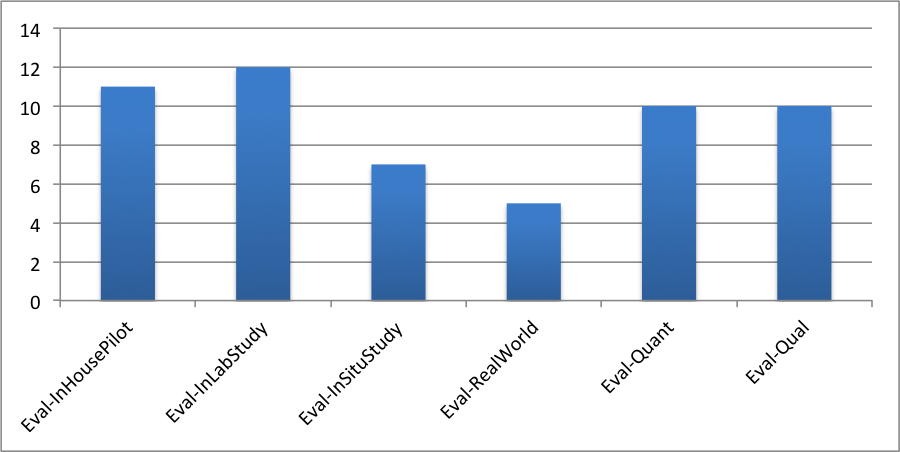
\includegraphics[height=2in]{SurveyEvalTechniques}
%     	   \caption{Responses for evaluation techniques used (N=16, \emph{``check all that apply''}).}
%     	   \label{fig:questionnaire:evaltechniques}
%     \end{subfigure}
%     \begin{subfigure}{\textwidth}
%             \centering
%             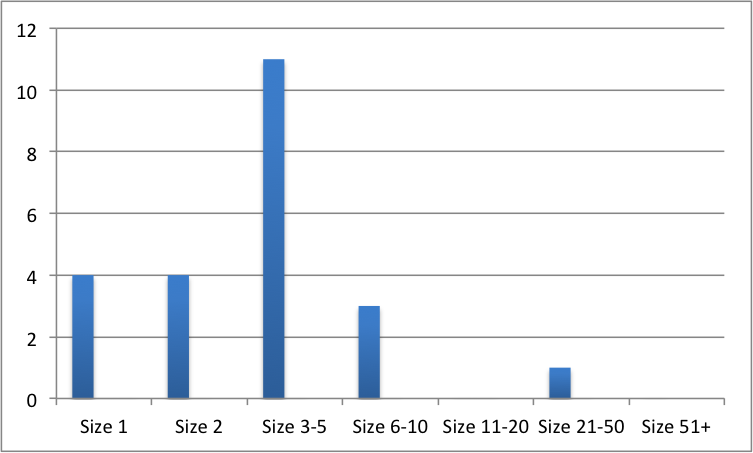
\includegraphics[height=2in]{SurveyGroupSize}
%     	   \caption{Reported group size for projects (N=16, \emph{``check all that apply''}).}
%     	   \label{fig:questionnaire:groupsize}
%     \end{subfigure}
% \end{figure}


\begin{figure}[htb]
    \centering
    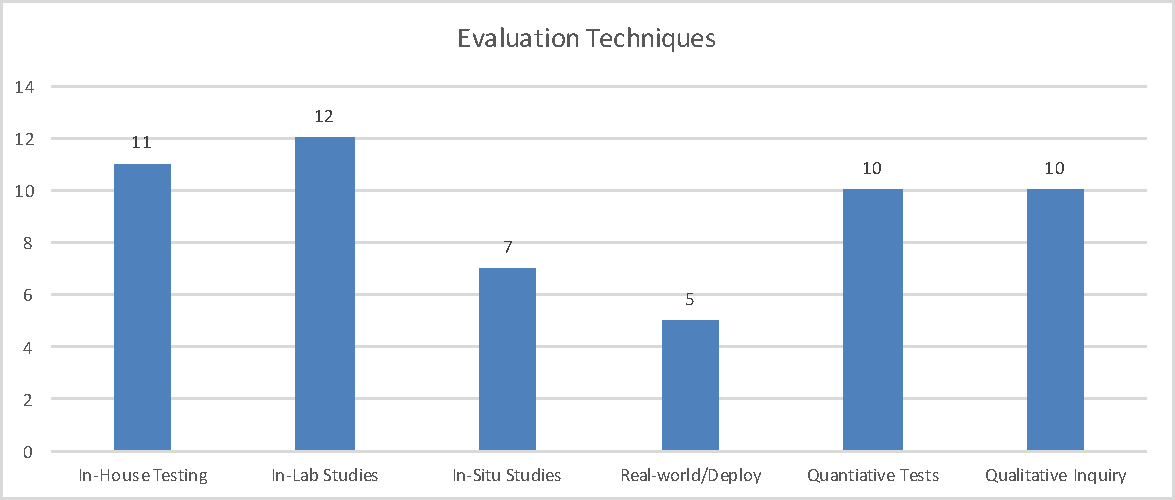
\includegraphics[height=2in]{SurveyEvalTechniques-2016-06-29}
   \caption{Responses for evaluation techniques used (N=16, \emph{``check all that apply''}).}
   \label{fig:questionnaire:evaltechniques}
\end{figure}
    
    
\begin{figure}[htb]
    \centering
    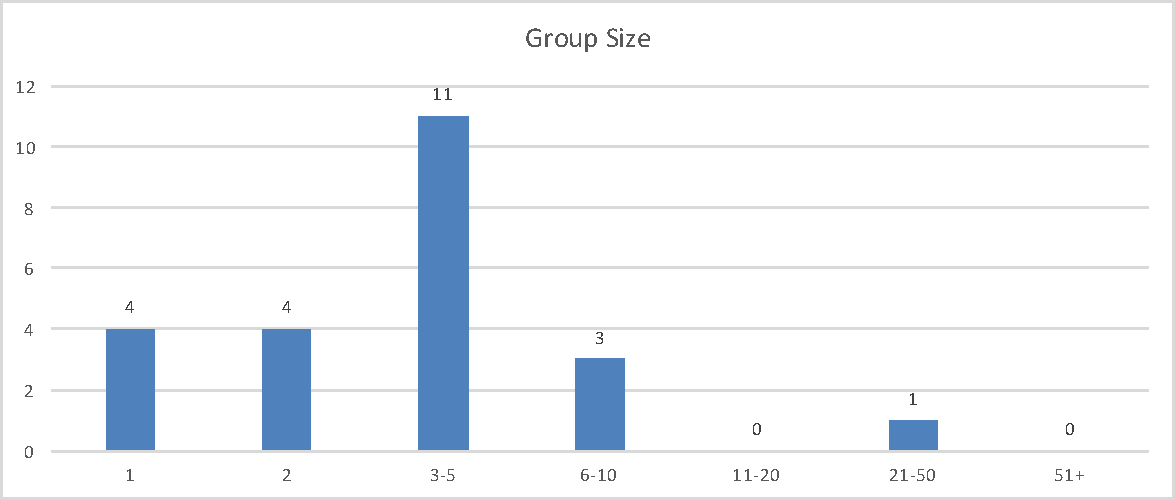
\includegraphics[height=2in]{SurveyGroupSize-2016-06-29}
   \caption{Reported group size for projects (N=16, \emph{``check all that apply''}).}
   \label{fig:questionnaire:groupsize}
\end{figure}




%%%%%%%%%%%%%%%%%%%%%
% Subsection: Qual Questionnaire Results
%%%%%%%%%%%%%%%%%%%%%
\subsubsection{Qualitative Data (survey \& brainstorming): Consistency, Quality, Value} % Results
\noindent
%
Qualitative responses from the survey's first open-ended question, which asked for the largest challenges participants faced in haptic experience design, highlighted three themes\revOne{:} 
%\kmC{07.23: hard to follow, slc} % not knowing  gist of  questions that generated these responses. Can you summarize, and also it might be appropriate to refer to the questionnaire itself in an appendix. Might be possible to repeat the full question as each list item.}
%% KM 16.14: by 'qualitative responses', do you mean written on questionnaire? Reader could use a reminder of where this came from. The list doesn't sound like things people would say in conversation. Maybe in a panel, but the panel wasn' defined.
%
\begin{enumerate}
\item \textbf{Universal design}: \qqquote{universal experience}, \qqquote{adopting wide spectrum of users}, \qqquote{optimal and consistent delivery of haptic cues to large number of people}, \qqquote{users variations in terms of subjective analysis}, \qqquote{common haptic experiences, any person/any device}, \qqquote{the spectrum of perception}.

\item \textbf{Evaluating quality}: \qqquote{what is `good enough'?},
\qqquote{modeling haptic quality of experience},
\qqquote{appropriate fidelity force feedback},
\qqquote{optimal and consistent delivery of haptic cues...}. 

\item \textbf{Value}: \qqquote{getting people to realise the benefits of good haptics. Finding new ways to use hi-fidelity (wide bandwidth) haptic feedback to enhance UX},
\qqquote{Bringing haptics to mainstream/consumer electronics},
\qqquote{merging the technologies, make safety and pleasure experiences},
\qqquote{convincing it's useful}.
\end{enumerate}

%\kmC{07.23: clarify - were the terms above responses to three distinct questions? slc} % or are they subthemes you found in answers to, eg, a single question? Specifically: make clear how much experimenter involvement there was in the organization into these three bins (above) and the 'other' bin below. Why not include Emotion and Language in your list above?

\noindent
%\kmC{where were they made, in the survey?}
Other responses include emotion (\qqquote{transfer emotion through haptics}) and language (\qqquote{haptic language; no simplicity in generating new sensations}).
In the second open-ended question, which asked what participants would like to see in a design tool to overcome these challenges,
%\kmC{slc: ideas for a design tool},
%% I'd like to hear more on the question here (e.g., "ideas for what a design tool might provide" because the quoted terms don't seem to fit will with question I imagine. A more general problem may be that some of the quoted terms are just hard to understand.
respondents suggested ways of handling variability or  definability, such as automatic configuration: %, were the main requests for design tools:

\begin{quote}
    \qqquote{mapping},
    \qqquote{automatic evaluation of systems and actuators},
    \qqquote{quatification [sic] of haptic perception},
    \qqquote{autoconfiguration, calibration and prediction of results with the users},
    \qqquote{accessible to all, supported by standards},
    \qqquote{autoconfigure depends that perception [sic]},
    \qqquote{bigger testing pool}.
\end{quote}


Many of the challenges identified during brainstorming mirrored questionnaire results.
Three groups (G1,2,6) focused on the \textit{value} of haptics: what is the point or benefit % goal 
in certain situations; as well as how to market that advantage to either a client or end-user.  % , and how to market haptics.
One group (G3) tackled the problem of \textit{examples of good design}, including hardware and software architecture, suggesting a repository like GitHub or software engineering patterns.
Three groups (G4-6) talked about \textit{meaning} -- and subjectivity therein, including the possibility of a shared or useful language.

\revOne{The workshop discussion suggested that} %The follow-up discussion developed these challenges further. 
%Emergent themes were that
% reinforcing that 
haptics is not well marketed and that touch is taken for granted. The word ``haptic'' might be too jargonny or poorly understood; perhaps other terms like ``tactile effect'' or ``physical effect'' could be more useful.
Curated examples and an on-line repository were offered as valuable goals.
% seemed like valuable goals as well.



\revOne{Our findings from this second study confirm those from the first.
Hapticians face barriers from communication and an understanding of the value of haptics; variability in used tools, targeted hardware and individual perception; and a desire for more powerful tools that can automatically create or evaluate haptics, or use and share examples.}

% \osC{Todo: post-it analysis}



%%%%%%%%%%%%%%%%%%%%%%%%%%%%%%%%%%%%%%
%
% Section: Discussion
%
%%%%%%%%%%%%%%%%%%%%%%%%%%%%%%%%%%%%%%
\section {Discussion}
\label{sec:discussion}
\noindent
%
As a first step in further exploring the findings from our \revOne{two studies}, 
we examine in more detail the critical activities practiced by \revOne{hapticians}.
This inventory confirms that \haxd is a field of design with familiar processes, but also one that is developing its own identity distinct from general UX design.
We then identify major challenges encountered in \haxd that are unique to or exaggerated when the experiences being designed are haptic. % with haptic experiences.
We conclude with several concrete recommendations to support \haxd in the future and a vision for what this might look like.
\revOne{These findings can inform future efforts to understand and support hapticians.}


We note that our interview results were generally applicable to professional haptic design in 2012.
Based on recent interactions with designers in comparable roles (including % especially % ?? doesn't make sense
those in the workshop), \revOne{and our own experience as hapticians ourselves,} we believe our findings continue to hold at the time of writing (2016) with three caveats: (1) hardware has improved and become more diverse, (2) haptic feedback is more prevalent and more expected in the consumer culture, and (3) in a limited number of sub-disciplines, such as gaming environments and movie special effects editing, specialized tools have begun to appear to solve very specific designer problems where the cost/benefit equation merits their use. 
However, the design pressures shaping practices and tools themselves have changed little over that time, as \revOne{shown} by our findings from the more recent workshop (2015, Section~\ref{sec:workshop}).

%\kmC{07.23: major high level comment: conspicuously absent is any highlighting of what's good about haptics -- what IS this elusive value? slc} % while it's true we're focused on what it is that designers do (as opposed to their product) and thus what's hard about it will naturally float up, the overall impression I have at this point is one of considerable negativity. Little has been said about the payoff of including haptics in design, nor any ways in which haptic design is easier or more rewarding than other modalities. Why bother with all this? Is it worth it?

\subsection{Activities of Haptic Design}
\noindent
% From the observations reported here, 
Based on our observations, we report
% Original text:
% this work, and **previous work on HaXD tools**, 
% Alternative text: "From the observations reported in this work, we are able to extract several classes of activities that haptic designers conduct, all familiar..."
% I *think* this is the first mention of using data from 'previous work on HaXD tools' (see orig text above). Need way more clarity on what this consists of, and it must be introduced before this point.
%
% we suggest
the following activities that haptic designers conduct, all familiar to designers in other fields.

%\kmC{08.01: question boldface highlights in this section. They do pop nicely but consider contrast to later sections.}

\begin{description}
    \item[Develop and communicate vision.]
    \revOne{Hapticians} must articulate the value that their designs can bring to both end-users and customers.
    They must communicate value to their team and others and, crucially, % critically, 
    they must \poptext{persuade external stakeholders} that their product will contribute to the bottom line.
    To do this, they must \poptext{collect, run, and tune demos}, a critical part of the communicative toolkit for haptic designers.
    
    \item[Prepare for design.] \revOne{Hapticians} need to \poptext{divine requirements} from customers, which customers often do not understand themselves.
    \revOne{Hapticians} also \poptext{gather examples}, both to provide inspiration and facilitate communication.
    \revOne{Hapticians} need ways to capture, modify, manage, find, use, and share examples and ideas, both ones they develop themselves and ones they seek out for inspiration. 
    %\kmC{08.01: is last sentence part of Prepare?}
    
    
    \item[Iteratively develop, communicate and evaluate multiple concepts.]
    Our participants needed to iterate, often with their clients' and users' feedback to find the best designs.
    \poptext{Design thinking} and \poptext{user-centered design} % UCD 
    are both important to apply to haptics, especially because requirements are difficult to communicate and understand.
    % Both \textbf{sketching} and \textbf{refinement} are needed.
    Additionally, \revOne{hapticians} must either \poptext{communicate with engineering},
    articulating requirements to receive new physical prototypes, or \poptext{have engineering skills} to create demos and prototypes themselves.
    During iteration, hapticians must also \poptext{evaluate designs and collect feedback},
    both with informal feedback from colleagues, and formal studies, typically run by a UX/research division.
    However, this practice is currently constrained both by industrial concerns (confidentiality, cost, end-user access) and the hard-to-share nature of haptic technology itself.
    
    \item[Interface with research.]
    Hapticians need to \poptext{hand off} prototypes or stimuli to their UX or research division, and communicate study goals.
    They must also \poptext{monitor the academic research} in this rapidly changing field, interpreting data emanating from multiple sources: marketing research, psychophysics studies on hardware and stimuli, and interaction design of applications. 
    % from studies from multiple sources: marketing research, feedback on prototypes and stimuli, and monitor the academic research in this rapidly changing field.
    Alternatively, as with engineering, they might \poptext{plan, run, and analyze studies}  directly.
    
    \item[Manage IP.]
    \revOne{Hapticians} must be sensitive about intellectual property, both that of their company's technology, and of the many companies and divisions they interact with. This can involve deliberately \poptext{exploiting or avoiding particular design approaches}; and has heavy implications for \poptext{confidentiality and privacy} of their overall process.

\end{description}




\subsection{Challenges for Haptic Experience Design}
\noindent
%
From our \revOne{two studies,} %interview and the subsequent workshop findings, 
%\kmC{07.23: since researcher extracted the themes, state differently? slc} % seems more appropriate to say "from themes extracted from our participants' accounts - to honestly acknowledge the researcher's involvement in process, ie potential for getting it wrong.
we identify several challenges facing \revOne{hapticians} that are unique to \haxd or are exacerbated when working with haptics compared to non-haptic UX design. 
%\kmC{07.23: wondering if these are too redundant/repetitive with earlier development. Definitely try to at least tighten. Depends in part on whether we expect (and will recommend that) skimming readers to jump over 2-4, with 5 almost standing alone.}
%\osC{08.01: I think these are tighter, higher-level, and less redundant now.}




% \begin{enumerate}

    \subsubsection{Context is largely unknowable}
    \noindent
    % \item[\textbf{C1}] \textbf{Context is Unknowable.} % \textbf{Unknown Context.}
    Haptic experiences are multimodal and holistic, % even I'm not sure how to interpret 'vertical' here (vertical in what dimension? it sounds like the opposite of vertical -  you're saying it interacts with everything, not with some specific dimension), and to many readers the term will be jargon in any event.
     interacting closely with physical hardware, grip, and orientation.
    When our participants knew the haptic experience's physical context, like the dashboard of a car,
    %\kmC{07.23: see earlier comments about `context'. which one are you referring to here?}
   they were able to use tricks to improve designs and circumvent constraints. % from section 3, see my concerns about what these terms are being used to represent. The awkwardness continues here - this is not the ONLY thing they used, surely!
     %to improve their sensations.
    However, when context is unknown, \eg, due to confidentiality, %  relevant intellectual property or due to 
    diverse environments, applications and means of handling an interface, % grips, 
    hapticians \revOne{are} hampered in their attempts %  very limited -- especially when trying 
    to create consistent experiences.
    
    \subsubsection{Applications and individuals vary a lot}
    \noindent
    % \item[\textbf{C2}] \textbf{Individuals Vary.} % \textbf{Individual differences.}
%    \kmC{07.23: this one was barely mentioned before now- disproportionately low attention.}
    There is no ``one size fits all" in haptic experience design.
    Each customer's design challenge has new properties.
    Hapticians must continually adapt their practice to changing conditions \citep{Schon1982}, and cannot simply design once and deploy.
    Companies use haptic sensations to brand their products, and individuals might want to customize effects for their preferences:
    users perceive, understand, and respond affectively in different ways to a haptic experience.
    %Different people, who experience perceptual differences based on age, sex, and their need-for-touch, will have different responses to a haptic sensation.
    %Moreover, their past experiences affect how they will interpret a sensation, \eg, feeling a vibration as a cat's purr or a car's rumble.
    %This has both an effect on end-users and on customers, as each application area needs the haptic technology to be tailored, hindering production at scale.
    
    \subsubsection{Demos are complex, costly, and crucial}
    \noindent
    % \item[\textbf{C3}] \textbf{Demos are complex, costly, and crucial.} % in-person.}
    % Despite being 
    Essential in eliciting requirements, communicating vision, and persuading customers, demos are %especially effective when tunable or customizable. However, they are
    % demos are 
    hard to manage.
    With many moving parts and ways to fail, demos often require a dedicated assistant;
    latency is a special challenge for early prototypes, and can defeat carefully synchronized multimodal effects. %the prototype's objective of
    %making an experience real. %  trying out the experience.
    Because \haxd takes place over global distances, %internationally 
    and across  organizations and disciplinary boundaries, %secrecy concerns and remote collaboration,
    it is often difficult to have a handler onsite, send proprietary hardware, or divulge enough detail for clients to run them on their own. % we can't always have someone present to nanny a demo.
%   Once setup, however, they seem to be effective, especially if they are tunable or customizable.

    \subsubsection{Iteration is painful}    
    \noindent
    % \item[\textbf{C4}] \textbf{Iteration is painful.} % \textbf{Painful iteration.}
    Every change to a haptic experience results in a change to the ``guts'', including reinforcing modalities and physical setup;
    % Tight technical constraints, like low latency, need to be followed to be effective.
    technical constraints are tight and unyielding.
    % This means that iteration is slow and difficult.
    Hence, even early `sketching' iterations to understand requirements can be slow and difficult, limiting playful exploration of a design space and disrupting communication with customers and users. %, yet continual iteration is essential throughout a design process.
    %However, 
    %Customers and users don't understand requirements without trying ideas. %, and haptic technology must be tailored to each application.
    % Thus, rapid iteration or parallel development is essential to get things feeling ``just right''.
    % Despite this, iteration remaines painful; special care is taken by our designers to allow for easy tuning, but better solutions remain to be seen.
    
    \subsubsection{Barriers to interdisciplinary collaboration are significant}    
    \noindent
    % \item[\textbf{C6}] \textbf{Barriers to interdisciplinary collaboration are significant.}
    % Haptic design is extremely multidisciplinary.
    Hapticians either need to fill many roles or work in groups that include hardware, software, design, business, and psychology.
    Furthermore, haptic design teams must interact with many external stakeholders stratified across different international companies, encouraging remote, asynchronous collaboration with physical, synchronous designs.
%    \textit{Making} skills, including engineering, are especially valuable 
 %   \kmC{07.23: not sure this point has been made earlier / substantiated?} 
  %  but often segregated from the central design group.
    %This leads to a knowledge discontinuity %, where hapticians must handle every role, or know ho%exacerbated by the need for haptic technology to be % Especially because haptic technology needs to be 
    %tailored to each problem: we cannot design once and forget. %  and need to maintain multidisciplinary groups.
    
    
    \subsubsection{Cost/benefit ratio is not obvious or easily quantifiable}    
    \noindent
    % \item[\textbf{C5}] \textbf{Cost/benefit ratio is not obvious or quantifiable.} % persuasive. - KM 07.23: seems misuse of 'persuasive'. Perhaps, 'does not persuade clients', but that suggests that there is in fact no good reason to include haptics. I think the more accurate situation is that it's hard to slap a $$ value on it. 
    % Haptic technology, ironically, often provides  intangible benefits: 
    The benefits of haptic technology are often intangible: better user experience, usability, branding, or perception of quality.
    %Further, it is
    % Designers are tasked with persuading 
    Product manufacturers (phones, cars) must be convinced of the contribution to the bottom line, and % than users themselves who must be convinced of them.
    are all too aware that improving haptics comes with increased cost and risk.
    Haptic design teams reaching out to customers through risk-adverse engineering avenues face additional push-back. %especially in light of low % without a way to tie benefit directly to increased revenue or profit.
    %A generally low profile and
    %awareness of haptic technology among consumers, limited infrastructure and inability to articulate needs or design intentions. % KM: state it as a challenge, not a solution or goal. And logically connect the sentence clauses.
    % Lack of infrastructure, public awareness, and ability for people to  say what they need or intend means we need to establish haptics more prominently in the public consciousness.
    
    
    \subsubsection{Evaluation methods are limited and often not pactical}
% \item[\textbf{C7}] \textbf{Evaluation methods are limited and often inaccessible.}
    \noindent
    Quality of experience, usability, and branding are difficult to study with physical systems.
    Although many of our participants mentioned evaluation methods as important, time and cost constraints limited it in practice; % how much evaluation is conducted. Typically, 
    acceptance testing seemed to be the primary tool. % result.
    Hapticians use both qualitative and quantitative methods, but \emph{in-situ} evaluations are difficult to come by, suggesting that haptic designers primarily conduct evaluations in-lab and do practical deployments. %., but not analytics or context-based investigation.
% \end{enumerate}



\subsection{Recommendations for Haptic Experience Design}
\noindent
From these challenges, we identified three main directions for development which % implications that 
could lead to better haptic design in the future.
% developing adaptable haptic interfaces, exploiting virutalization of physical phenomena, and establishing better conceptual infrastructure.

\subsubsection{Develop adaptable haptic interfaces}
\noindent
    Many of the challenges facing \revOne{hapticians} are a result of uncertainty or variability in physical context.
    One solution is to  let physical haptic interfaces adapt their context, either automatically or with help from a designer, customer, or end-user.
        
    One automatic approach to mitigate variable physical context is to employ \poptext{closed loop control}: adapt actuator output to desired levels with sensors.
    For example, a microphone could  sense the external vibrations of a VT actuator, {whose}  output can then be modified to overcome the effect of external factors like material, orientation, and grip and achieve a specified frequency, amplitude and responsiveness. 
    This might be deployed in products during use, or once during manufacturing as quality assurance to adapt for different product materials.

    Another approach is to let the customer or user adapt the experience through \poptext{customization}; this can handle  both physical context and individual differences in perception and preference.
    This might be a simple volume control, or a powerful menu of settings.
    Customizable infrastructures that support fine-tuning can also help speed iteration once demos or even fully-fledged applications are set up, letting designers and customers try variations of a haptic experience easily.

    Finally, \poptext{efficient calibration} of demos, using either sensors or a person's input, could improve collaboration with easier demo or product setup.
    %\eg, evaluation kits where customers and clients can experience demos without a sales representative being physically present to orchestrate the experience.
    Devices that are self-assembled or operable by non-experts require an easy way to troubleshoot and ensure correct rendering. 
    This could engage the DIY community to explore haptic technology, and improve efficacy of sending evaluation kits to potential customers.


\subsubsection{Exploit virtualization}
\noindent
    The unique problems of haptic design stem from the combination of % their 
    physicality and the software engineering % programming
    necessary to integrate the hardware into a solution.
    % They  often inherit challenges of both physical objects and complex software engineering. \osC{ugh bad writing}
    % To reduce these challenges, one could try to offload challenges into 
    Some of these challenges may be offloaded through virtualization:
    certain types of iterations or tests can be done more efficiently with software simulations or crowdsourced evaluation -- once this capability exists.
    %\kbE{virtualized software to substitute one technique for another, thus} circumventing their physical limitations. 
    %\kbC{I don't follow the point here. How does virtualizing software avoid a physical problem?}

    \poptext{Proxies} are one way to virtualize complex physical setups,
    \eg, using low-fidelity feedback like phone vibrations when high-fidelity feedback is unavailable~\citep{Schneider2016hapturk}.
    Low-fidelity previsualization of haptic sensations (or ``pre-feels'') ~\citep{Schneider2015} can improve iteration speed, by allowing the designer to experience an approximation of  an iteration before committing resources to building it, and/or to compare with a reference starting point.
    Visual or audio proxies can easily exploit existing infrastructure.
    
    
    \poptext{Software simulations} of hardware can explore how different electronic or mechanical components could be rearranged to preserve or enhance dynamics, reducing physical prototyping.
    Even more advanced might be the use of simulations to develop ``perceptually transparent'' sensations~\citep{Ryu2007}, allowing actuators or other components to be swapped in and out if upgrades or cheaper models are available, while software components are automatically updated to achieve a consistent end result. 
    %\kmC{?? slc} % explain why you'd want to swap out hardware components if not to change the feel. Perhaps you'd want to use cheaper components but then the question is whether the same performance can be achieved. The natural approach there would be to run component specs through the simulation, get a yes/no/by how much kind of answer, then verify the best candidates in hardware. 
    This virtualization technique dovetails nicely with closed-loop adaptable interfaces by establishing models and correcting for errors.
    
    Software has enabled immediate, efficent deployment of visual and audio stimuli through the Internet.
    Analogous \poptext{infrastructure} could help haptic technology catch up to other modalities more quickly, \eg,
    developing modular systems, data structures and protocols, and large on-line repositories of examples.
    \poptext{Broadcast} haptics  remains an important and unrealized goal, which can help both with potential customers and end-user experiences~\citep{Modhrain2001}.
    
    % \item[\textbf{R7}] \textbf{Find the ``killer app''.}
    % \kmC{I don't like this one. slc} % I stopped believing in the "killer app" a long time ago. I really doubt there's ever going to be some single application that will be valuable or popular.. 
    % % furthermore, you think people haven't been on this quest already for 20 years now? As a recommendation, it's sort of like recommending someone to "win big" without any clues about how.
    % % if you must have this, suggest calling it something like a "breakthrough opportunity", and list it not as a recommendation, but a comment at the end where this commonly known thing is reiterated. Try to add some value to it - what properties must this breakthrough application have? A long-time obstacle is that we're mainly finding places where haptic feedback can play a support role, but few where it's essential; the support doesn't justify its cost. For example, wearables are a big deal for haptics because they start to bring together factors where its disadvantages are diminished and it may have value on its own. 
    % To help persuade customers (C5) and promote haptics, there still needs to be a killer application that catches the popular imagination.
    % Although haptics has enjoyed great success in training environments, professional applications like remote surgery, and widespread adoption of basic vibrations, ``personal haptics'' has yet to achieve the same motivating traction that was found in personal computing with the spreadsheet. %VisiCalc
    % This need not be an application, it could also be studies that relate the benefit of haptics to the bottom line.
    
    
\subsubsection{Establish richer conceptual infrastructure}
\noindent
Several measures can help to address communication and cultural barriers to haptic design. % we propose promoting haptics outreach and education, developing a haptic design language for different stakeholders, and improving evaluation techniques.

    \poptext{Outreach and education} might be able to improve perceived value of haptics and facilitate interdisciplinary communication. %required by haptic design teams (C6) is to perform more outreach.
    Public haptic portfolios, accessible haptics education \citep{Jones2014} like online tutorials, support for DIY and maker cultures, and events like haptic hackathons \citep{madelska2015news} will help to establish haptics as a known term, spread the word about its value, but more importantly help more people join the conversation in which we will articulate % to find 
    the value in touch-based technology.
    It will help provide different stakeholders with common reference points, language, and understanding, both lowering the bar to conduct haptic design as a team member, and by providing a voice to external stakeholders.
    
    
    A \poptext{haptic design language} is needed for multidisciplinary team member and client communication (C6).
\revFinal{A design language, like Google's Material Design (\url{https://material.google.com}), is a defined set of aesthetic and interactive rules to ensure a consistent look-and-feel.}
    Much like graphic design, where non-experts might be aware of some concepts (symmetry, contrast, hot/cool colours) 
    while experts know much more (colour combinations, concept of weighting in a visual design), 
    a shared, objective and teachable language will help teams communicate across divisions and with clients, users, and customers.
    It remains to be seen whether this will be a formal lexicon of terms, or ideas that emerge organically; either way, we suggest paying careful attention to the language used when doing haptic design, and to share the language alongside the sensations and their components.
    
    
    \revOne{Hapticians} have limited access to \poptext{evaluation techniques} that are taken for granted in other modalities, especially \emph{in situ} tools.
    Promising ways of mitigating this handicap is application of remote analytics to haptic design, \eg, logging, machine learning, or qualitative contextual inquiry.
    This may require development of new batteries of haptics-suitable tests, especially ones which target its less objective benefits (\eg, quality and branding), which might in turn help to study perceived value and risk.


\subsection{Future of Haptic Design}
% \noindent
%
% Through this inquiry, we have found two main clusters of findings: how design thinking has been and can be further applied to haptics, and 
% \kmC{adequately covered? slc: intrinsic differences from other fields.} % I'm not sure this last one got very explicitly covered. ???
% Together, these help us develop a roadmap to establishing haptic experience design as its own field.

% \subsubsection{Applying design thinking to haptics}
% \noindent
\noindent Hapticians follow an observable, defined process.
They collect requirements, develop multiple concepts, and iterate until they arrive at a final experience, which is then evaluated with varying amounts of rigour.
We saw evidence of libraries, examples, and our participants' own craft and experience; we also saw a diverse, international, collaborative ecosystem.
Some deliberately applied user-centered design techniques.

However, we also see that haptics \qquote{P3}{might be 30 years behind graphics}, or at least \qqquote{really new}, \ie, in an early stage of development.
% By drawing analogies to other, more established fields of design, we can see areas to improve.
% Hardware is  improving, but we face many barriers from the youth of the field: \kmC{just repeating challenges? low value.}
% \begin{enumerate}
%     \item software and hardware infrastructure aren't in place
%     \item limited language with which to talk about requirements, goals, and sensations
%     \item secrecy. by working with novel technology, IP plays a central role hindering collaboration
%     \item Painful iteration cycles
%     \item value proposition not understood
%     \item risk of developing verticality with something new and unproven
%     \item branding, documentation is early stages (how do we talk about it?)
%     \item ...
% \end{enumerate}
%
%
% \subsubsection{What's different about haptics?}
% However, by applying design thinking to haptics, we also find intrinsic challenges tied to the modality of touch, which are not faced by other fields of design.
%
% \kmC{Are these adequately supported by previous sections? I expected more explicit development, based on opening.}
%
% These are:
% \begin{enumerate}
%     \item Problem of representation
%     \item Problem of context (ramped up to \kmC{??: ten})
%     \item Problem of multimodality (touch is especially overridden)
%     \item Problem of multiple senses (tactile, kinesthetic) synthesized
%     \item Active exploration
%     \item Verticality - software + hardware, and associated risk and collaborativeness
%     \item interdisciplinariness (from some of the above, also a problem of youth of the field)
%     \item irritation
%     \item customization
%     \item consistency (context + customization/individual differences)
%     \item changes to the guts - can't just swap in new hardware (tied to context)
%     \item another context point: need the entire experience to evaluate, describe, or persuade (multimodality + context + early days)
%     \item ...
% \end{enumerate}
% A vision of \haxd as a fully-developed field is exciting but challenging,
% \kmC{07.23: has 'exciting' been sufficiently justified?}
% at a time when experience design in general is still finding itself.
We believe that \haxd can draw from both newer fields like experience and interaction design, as well as more established ones like graphic design.
How might it look?

\revOne{Hapticians} might work in teams, interacting with other relevant units.
%\kmC{?creative, product design?}.
From our research, it is likely that \revOne{hapticians} will need to %\kmC{?need to be vertical? slc}, % here, you're using 'vertical' to indicate need to interact with different parts of the food chain. My problem with this term is still that it's not really a chain, it's more like a savannah with interactions in every direction - just doesn't fit.
 communicate with  everyone from mechanical engineers and software developers to people conducting business and user research.
As with graphic design schools, there may be formal education available for haptic designers.
However, as haptic technology needs to be tailored to each specific problem, these will likely be generalized professional programs that train diverse skills, or will focus on certain sub-categories of haptic technologies, \eg, tactile artists or animators~\citep{Schneider2015}, friction designers, or 3DOF force-feedback developers.
As hardware becomes more affordable, we also expect the recent Maker movement will encourage hobbyists and artists to explore haptic technology and push its limits. % , possibly in the near future.

As with other emerging media, such as the web browser wars of the 90s, standardization of HTML/CSS, and Blu-Ray versus HD DVD, we expect diverse file formats and infrastructures to emerge and then coalesce.
Given the diversity of haptic technologies and experiences, we expect these to be centered around \emph{paradigms}, mental models of how to work with a haptic experience.
For example, haptic icons~\citep{MacLean2003} are one paradigm: display-only, temporal and meaningful entities rendered on a single body location. These might be designed, distributed, and experienced similarly to audio files.
Tactile animations~\citep{Schneider2015} are another: generalized spatio-temporal entities that can be rendered continuously on different grids.
Multi-DOF force-feedback displays are often programmed with a third paradigm: a virtual environment and a single manipulator; this is most analogous to 3D virtual worlds.
Paradigms can be applied to multiple devices in a class (\eg, tactile animations on grid displays), or multiple paradigms might apply to a single device (a Haptuator~\citep{Yao2010}) can display a haptic icon (temporal only), or it can produce a directional force~\citep{Culbertson2016} (spatio-temporal).

We expect design dimensions to be further developed, and eventually encapsulated into best practices, just as alignment, contrast, and weighting are used for graphic design.
Other design languages, like musical notation, will facillitate recording and communication amongst experts.
Meanwhile, more developed aesthetic theories, like musical  or colour theory, will help guide people to effective, pleasing, differentiable haptic designs.
Intellectual property law will need to be adapted -- much like a logo can be trademarked, how might a certain button click? 
Whether a haptic icon set should be protected, and how to set an appropriate level for burden of proof, remain open questions.
We hope that these questions and more will be answered during this exciting time for one of our most essential senses.



% They will need access to both research and engineering resources, and may need to fill those roles themselves, or communicate effectively with more specialized teammates.
% They will need to develop a vision for an experience, develop initial sketches and concepts, iteratively refine multiple concepts, receive feedback, and communicate that vision effectively with stakeholders.
% They will need to capture, store, and manage examples or candidate ideas, both internally and when trying to browse.
% They will also need to fit their final designs into produce or experiential infrastructure.
% From these challenges, we can start to see the path to a full field of design.

% 1) First, the community should continue to make progress developing hardware, control methods, tools, and exploring psychology and application areas.
% Many very smart people have made excellent progress, and we expect this to continue.

% 2) Next, we need to focus on ways to help the field catch up, focusing on problems of the field's youth.
% What can we learn from recent work in other, more established fields of design, such as ... ?

% 3) Finally, the biggest challenge is in handling intrinsic challenges, which will continue to be revealed as as follow steps 1) (studying the nature of touch and building haptic experiences) and 2) (studying design).
% \osC{Todo: Think hard about this section, it seems like the ultimate capstone for this paper + my dissertation.}.
% \kmC{Agree. Is part of the solution to organize the 'challenges' and 'recommendations' more along the lines of youth/intrinsic lines? What if you discussed both in the context of a 'grand challenge' (or killer app if you must): what makes breakthrough so darn hard? 
% }

%If we are able to do these things, imagine all the people-le-le, living for haptics \osC{Todo: Second part of final capstone, what would a world with haptic design be like, and how could we all benefit?}


% % Table
% \begin{table}%
% \tbl{Simulation Configuration\label{tab:one}}{%
% \begin{tabular}{|l|l|}
% \hline
% TERRAIN{$^a$}   & (200m$\times$200m) Square\\\hline
% Node Number     & 289\\\hline
% Node Placement  & Uniform\\\hline
% Application     & Many-to-Many/Gossip CBR Streams\\\hline
% Payload Size    & 32 bytes\\\hline
% Routing Layer   & GF\\\hline
% MAC Layer       & CSMA/MMSN\\\hline
% Radio Layer     & RADIO-ACCNOISE\\\hline
% Radio Bandwidth & 250Kbps\\\hline
% Radio Range     & 20m--45m\\\hline
% \end{tabular}}
% \begin{tabnote}%
% \Note{Source:}{This is a table
% sourcenote. This is a table sourcenote. This is a table
% sourcenote.}
% \vskip2pt
% \Note{Note:}{This is a table footnote.}
% \tabnoteentry{$^a$}{This is a table footnote. This is a
% table footnote. This is a table footnote.}
% \end{tabnote}%
% \end{table}%


%%%%%%%%%%%%%%%%%%%%%%%%%%%%%%%%%%%%%%
%
% Section: Conclusion
%
%%%%%%%%%%%%%%%%%%%%%%%%%%%%%%%%%%%%%%
\section{Conclusion}
\noindent In this paper, we provide a first picture of how haptic experience design (\haxd) is being practiced in industry.
We report findings from interviews with six \revOne{hapticians}, finding observations about designer process and themes about the holistic nature of haptic experiences and the collaborative ecosystem and cultural context of our participants.
We supplement this with broad follow-up data from a recent workshop at a major haptics conference.

We identified the various activities \revOne{hapticians} practice, similar to other fields of designer.
We also note specific challenges facing designers who work with haptics, and recommend both high-level priorities and low-level tactics for % make recommendations for 
conquering those challenges.
This contribution is a first step in understanding \haxd outside of the research lab; we look forward to when physical, interactive technology can be designed with creativity, passion, and panache.


% Appendix
% Acknowledgments
\section{Acknowledgements}
\noindent
We deeply thank our designer participants for their time and dedication, Gordon Minaker for helping with survey distribution and workshop administration, and Hasti Seifi for helping to conduct the workshop brainstorming.
% \kbC{shouldn't this refer to the brainstroming session at the workshop, not the brainstorming itself? The latter is the ideas in this paper. The former was activity at the workshop.}
% \osC{Hasti was involved with both, I believe.}
% \kbC{How is what I have now?}
More broadly, we thank generations of our own lab's designers and our collaborators for the foundations they laid under these findings and ideas.
This research was supported by the Natural Sciences and Engineering Research Council of Canada (NSERC), the GRAND Network of Centres of Excellence, and the University of British Columbia's 4YF fellowship program. The user studies were conducted under UBC Ethics certificates \#B01-0470 and \#H13-01620.



\endinput
